\documentclass[11pt,a4paper]{article}
\usepackage[utf8]{inputenc}
\usepackage[T1]{fontenc}
\usepackage{mathpazo}
\usepackage[margin=2.5cm]{geometry}
\usepackage{amsmath,amssymb,amsthm,mathtools}
\usepackage{booktabs,enumitem,xcolor,array,needspace,caption}
\usepackage{placeins}
\usepackage[expansion=false]{microtype}
\usepackage{tikz,pgfplots}
\usetikzlibrary{arrows.meta,positioning,shapes.geometric,calc,fit,decorations.pathreplacing,backgrounds}
\pgfplotsset{compat=1.16}
\usepackage[most]{tcolorbox}
\usepackage[colorlinks=true,linkcolor=blue!45!black,citecolor=blue!45!black,urlcolor=blue!45!black]{hyperref}
\setlength{\parskip}{0.5em}\setlength{\parindent}{0pt}
\setlength{\emergencystretch}{2em}
\widowpenalty=10000 \clubpenalty=10000
\renewcommand{\arraystretch}{1.22}
\renewcommand{\topfraction}{0.9}\renewcommand{\bottomfraction}{0.8}\renewcommand{\textfraction}{0.1}\renewcommand{\floatpagefraction}{0.7}
\setlist{itemsep=2pt,topsep=3pt}
\newcolumntype{L}[1]{>{\raggedright\arraybackslash}p{#1}}

%---------- colours
\definecolor{cA}{HTML}{1F4E79}
\definecolor{cB}{HTML}{C0392B}
\definecolor{cC}{HTML}{1E8449}
\definecolor{cD}{HTML}{B9770E}
\definecolor{cG}{HTML}{7F8C8D}

%---------- theorem boxes
\makeatletter
\tcbset{labelfix/.style={before upper={\protected@edef\@currentlabel{\thetcbcounter}}}}% \ref now gives the theorem number, not the enclosing subsection number
\makeatother
\tcbset{thmstyle/.style={labelfix,enhanced,breakable,colback=cA!4,colframe=cA,boxrule=0.6pt,arc=1.5pt,
  left=6pt,right=6pt,top=4pt,bottom=4pt,fonttitle=\bfseries\sffamily\small,
  attach boxed title to top left={yshift=-2mm,xshift=4mm},boxed title style={colback=cA,arc=1pt,boxrule=0pt}}}
\newtcolorbox[auto counter,number within=section]{theorem}[2][]{thmstyle,title={Theorem~\thetcbcounter\ #2},#1}
\newtcolorbox[use counter from=theorem]{proposition}[2][]{thmstyle,title={Proposition~\thetcbcounter\ #2},#1}
\newtcolorbox[use counter from=theorem]{lemma}[2][]{thmstyle,title={Lemma~\thetcbcounter\ #2},#1}
\newtcolorbox[use counter from=theorem]{definition}[2][]{thmstyle,colback=cC!4,colframe=cC,boxed title style={colback=cC,arc=1pt,boxrule=0pt},title={Definition~\thetcbcounter\ #2},#1}
\newtcolorbox{intuition}[1][]{enhanced,breakable,colback=cD!6,colframe=cD,boxrule=0.5pt,arc=1.5pt,left=6pt,right=6pt,top=3pt,bottom=3pt,
  fonttitle=\bfseries\sffamily\small,title=Intuition,#1}
\newtcolorbox{caution}[1][]{enhanced,breakable,colback=cB!5,colframe=cB,boxrule=0.5pt,arc=1.5pt,left=6pt,right=6pt,top=3pt,bottom=3pt,
  fonttitle=\bfseries\sffamily\small,title=Warning,#1}
\theoremstyle{definition}
\newtheorem{example}{Example}[section]
\newtheorem*{remark}{Remark}
%---------- notation boxes and side notes (same visual vocabulary as the theorem boxes)
\newtcolorbox{notebox}[1]{enhanced,breakable,colback=cG!6,colframe=cG!75,boxrule=0.5pt,arc=1.5pt,left=8pt,right=8pt,top=5pt,bottom=4pt,
  fonttitle=\sffamily\bfseries\small,attach boxed title to top left={yshift=-2mm,xshift=4mm},boxed title style={colback=cG!75,arc=1pt,boxrule=0pt},before upper={\setlength{\parskip}{0.5em}},title={#1}}
\newtcolorbox{aside}[1]{enhanced,breakable,frame hidden,colback=cD!5,borderline west={1.8pt}{0pt}{cD},left=10pt,right=6pt,top=3pt,bottom=3pt,
  fontupper=\small,before upper={\setlength{\parskip}{0.55em}\textbf{\sffamily #1}\par\smallskip}}

%---------- status badges
\newcommand{\badge}[2]{\textcolor{#1}{\textsf{\footnotesize[#2]}}}
\newcommand{\proved}[1][]{\badge{cC}{proved#1}}
\newcommand{\modulo}[1]{\badge{cD}{proved mod.\ #1}}
\newcommand{\condl}{\badge{cD}{conditional}}
\newcommand{\openq}{\badge{cB}{open}}
\newcommand{\falsest}{\badge{cB}{false}}
\newcommand{\led}[1]{\textcolor{cG}{\textsf{\footnotesize(ledger #1)}}}
%---------- reading aids
\newtcolorbox{leadin}{enhanced,breakable,colback=white,colframe=cG,boxrule=0.5pt,arc=1pt,left=6pt,right=6pt,top=3pt,bottom=3pt,fontupper=\small,
  title={In this section},fonttitle=\sffamily\bfseries\small,coltitle=black,colbacktitle=cG!15}
\newcommand{\sectionbrief}[3]{\begin{leadin}\begin{description}[nosep,leftmargin=3.0cm,labelwidth=2.8cm]
  \item[Starting from] #1
  \item[Why this section] #2
  \item[Role in the paper] #3
  \end{description}\end{leadin}}

%---------- explained-edition boxes (added in this edition only)
\definecolor{cE}{HTML}{6C3483}
\newtcolorbox{explained}[1]{enhanced,breakable,colback=cE!4,colframe=cE,boxrule=0.6pt,arc=1.5pt,left=8pt,right=8pt,top=6pt,bottom=5pt,
  fontupper=\small,before upper={\setlength{\parskip}{0.45em}},
  fonttitle=\sffamily\bfseries\small,attach boxed title to top left={yshift=-2mm,xshift=4mm},boxed title style={colback=cE,arc=1pt,boxrule=0pt},title={Explained: #1}}
\newcommand{\edmark}[1]{\textsuperscript{\textcolor{cB}{\textsf{[#1]}}}}
\newtcolorbox{wstep}[1]{enhanced,colback=cA!3,colframe=cA!60,boxrule=0.5pt,arc=1pt,left=8pt,right=8pt,top=4pt,bottom=4pt,
  title={#1},fonttitle=\sffamily\bfseries\small,toptitle=1.5pt,bottomtitle=1.5pt}
\newcommand{\stepblock}[2]{\par\Needspace{6\baselineskip}\medskip\noindent\textbf{\sffamily Step #1: #2}\par\nopagebreak\smallskip}
\newtcolorbox{takeaway}{enhanced,breakable,frame hidden,colback=cA!3,borderline west={1.6pt}{0pt}{cA},left=8pt,top=2pt,bottom=2pt,fontupper=\small,before upper={\textbf{\sffamily Why it matters.}\ }}
\newtcolorbox{keypoint}{enhanced,breakable,frame hidden,colback=cC!5,borderline west={1.6pt}{0pt}{cC},left=8pt,top=2pt,bottom=2pt,fontupper=\small,before upper={\textbf{\sffamily Takeaway.}\ }}


%---------- macros
\newcommand{\R}{\mathbb{R}}\newcommand{\C}{\mathbb{C}}\newcommand{\N}{\mathbb{N}}\newcommand{\Z}{\mathbb{Z}}
\newcommand{\Ann}{\operatorname{Ann}}
\newcommand{\EP}{\mathrm{EP}}
\newcommand{\Eint}{E_{\mathrm{int}}}
\newcommand{\ring}{\mathcal{R}}
\newcommand{\Id}{\mathrm{Id}}
\newcommand{\Var}{V}
\newcommand{\dd}{\,\mathrm{d}}
\DeclareMathOperator{\Gcd}{gcd}
\DeclareMathOperator{\spn}{span}
\DeclareMathOperator{\dimc}{dim}

\pgfmathdeclarefunction{gauss}{2}{\pgfmathparse{exp(-(#1)^2/(2*#2))/sqrt(2*pi*#2)}}

\title{\textbf{Exact Recovery of a Linear Differential Operator\\ from a Single Solution}\\[4pt]
\large Identification, Factor Decomposition, the Interaction Term, and a Nonlinear Extension\\[2pt]\normalsize\textit{Explained edition}}
\author{}
\date{October 2026}

\let\oldsection\section\renewcommand{\section}{\Needspace{9\baselineskip}\oldsection}
\let\oldsubsection\subsection\renewcommand{\subsection}{\Needspace{7\baselineskip}\oldsubsection}
\begin{document}
\maketitle

\begin{abstract}
\noindent
Given one exact solution $u$ of an unknown differential equation in one space and one time variable, we ask what $u$ ``remembers'' about the equation. We answer in four steps. (i)~\emph{Identification}: for constant coefficients, $u$ determines its governing operator $P$ if and only if no partial quotient $(P/P_i)(\partial)u$ is an exponential-polynomial; no finite amount of data can certify this, and a black-box test is impossible, yet it becomes decidable with a modest extra hypothesis. (ii)~\emph{Decomposition}: $u$ splits into one component per irreducible \emph{factor} of the symbol, with an exponential-polynomial ambiguity of known finite dimension; the split is generally \emph{not} possible per additive \emph{term} of the operator. (iii)~\emph{Interaction}: for evolution equations $u_t=\sum_nA_nu$ with commuting terms the part of the solution due to the interplay of the terms has the exact form $\prod_n(\Id+\Delta_n)-\Id-\sum_n\Delta_n$ applied to the initial datum, it costs $O(N)$ per value but $\Theta(2^N)$ as a full table, and it is not a continuous function of the data in Sobolev norms. (iv)~\emph{Nonlinear} equations (Burgers, KdV--Burgers, Fisher--KPP) admit analogous statements, with sharp asymptotics across a shock.

\medskip\noindent We present the mathematics, the resulting algorithm component by component, a worked example, and the precise limits of the method. Every result carries a verification status.
\end{abstract}

\tableofcontents

\begin{notebox}{About this explained edition}
The text, theorems and numbering are those of the revised paper. In addition, \textbf{purple boxes titled ``Explained''} give a step-by-step reading of the surrounding material: definitions, small worked examples, and the intuition behind each result. They add nothing to the claims of the paper and can be skipped by a reader who only wants the statements.
\end{notebox}
\bigskip

%======================================================================
\section{Introduction}\label{sec:intro}
\sectionbrief
{one function $u(t,x)$ known exactly on a region $\Omega\subset\R^2$ (no noise), which solves $P(\partial_t,\partial_x)u=0$ for a constant-coefficient operator $P$ that is \emph{not} given.}
{to state precisely what we want from $u$ (three questions) and to give the reader a map of the answers before the details.}
{frames Q1--Q3, which are answered in Sections~\ref{sec:ident}, \ref{sec:fact} and \ref{sec:terms}; Sections~\ref{sec:nonlin}--\ref{sec:limits} extend and assemble them.}

\subsection{The question}
Let $u(t,x)$ be a function on a region $\Omega\subset\R^2$, known without noise, and suppose it solves a linear equation $P(\partial_t,\partial_x)\,u=0$. We do not assume $P$ is known. Three questions arise naturally.
\begin{enumerate}[label=\textbf{Q\arabic*.},leftmargin=1.1cm,nosep]
\item \textbf{Identification.} Can the operator be reconstructed from $u$, and when is the answer unique?
\item \textbf{Decomposition.} If $P$ is built from pieces, can $u$ be split into the parts that each piece generates?
\item \textbf{Interaction.} If the pieces are the \emph{terms} of the operator (diffusion, advection, \dots), what part of $u$ is due to \emph{no single term} but to their interplay, and can it be computed exactly and cheaply?
\end{enumerate}
The setting is deliberately analytic: no statistical model, no learned weights, no noise. The aim is an \emph{exact} procedure, and a precise statement of what is impossible.

\subsection{How to read the status labels}
Every statement carries one of the labels \proved{} (complete proof, independently reviewed), \modulo{X} (complete except for a cited published theorem~X whose source was checked), \condl{} (depends on an unverified lemma), \openq{}, or \falsest{} (a counterexample exists). The reviewers were independent AI agents, not human referees; fifteen core algebraic theorems were additionally machine-checked in Lean~4 (Section~\ref{sec:limits}). Grey tags such as \led{C3-T1} refer to entries in the project's claim ledger.

\subsection{Overview of the results}
Figure~\ref{fig:pipeline} summarizes the logical chain, read left to right: each box is a task, and each arrow is a theorem that allows the next task to be carried out. Table~\ref{tab:results} lists the main statements with their status; the rightmost column uses the labels just explained, and every row points to the theorem where it is proved.

\begin{figure}[!htb]
\centering
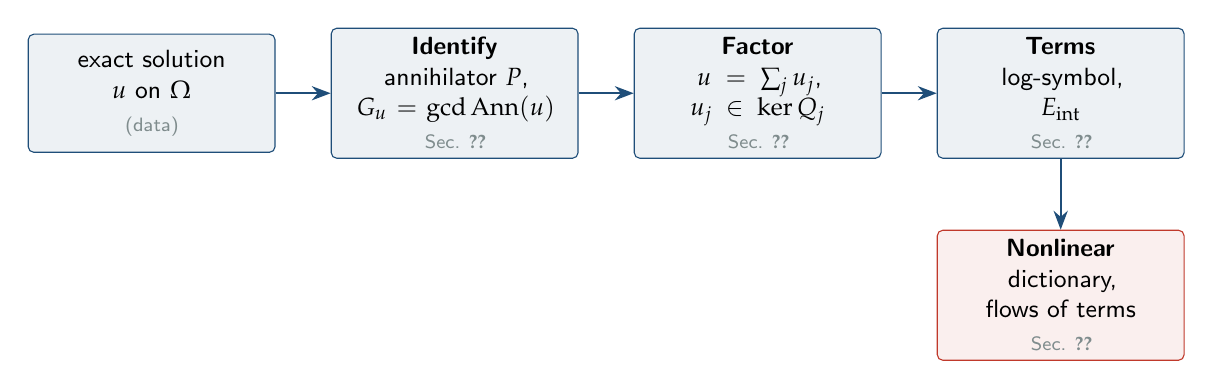
\begin{tikzpicture}[node distance=7mm,
  box/.style={draw=cA,fill=cA!8,rounded corners=2pt,minimum height=15mm,text width=2.9cm,align=center,font=\small\sffamily},
  arr/.style={-{Stealth[length=2.4mm]},thick,cA}]
\node[box] (u) {exact solution\\$u$ on $\Omega$\\[1pt]{\scriptsize\textcolor{cG}{(data)}}};
\node[box,right=of u] (id) {\textbf{Identify}\\ annihilator $P$,\\ $G_u=\Gcd\Ann(u)$\\[1pt]{\scriptsize\textcolor{cG}{Sec.~\ref{sec:ident}}}};
\node[box,right=of id] (fa) {\textbf{Factor}\\ $u=\sum_ju_j$,\\ $u_j\in\ker Q_j$\\[1pt]{\scriptsize\textcolor{cG}{Sec.~\ref{sec:fact}}}};
\node[box,right=of fa] (te) {\textbf{Terms}\\ log-symbol,\\ $\Eint$\\[1pt]{\scriptsize\textcolor{cG}{Sec.~\ref{sec:terms}}}};
\node[box,below=9mm of te,fill=cB!8,draw=cB] (nl) {\textbf{Nonlinear}\\ dictionary,\\ flows of terms\\[1pt]{\scriptsize\textcolor{cG}{Sec.~\ref{sec:nonlin}}}};
\draw[arr] (u)--(id); \draw[arr] (id)--(fa); \draw[arr] (fa)--(te); \draw[arr] (te)--(nl);
\end{tikzpicture}
\caption{Logical structure of the method. Each arrow is a theorem with explicit hypotheses, so a step can only be trusted under the hypotheses of the theorem preceding it. The three linear stages (blue) are followed by the nonlinear extension (red); the algorithm that chains them is in Section~\ref{sec:algo}.}\label{fig:pipeline}
\end{figure}

\begin{table}[!htb]
\centering\small
\begin{tabular}{@{}L{2.7cm}L{8.3cm}L{3.5cm}@{}}
\toprule
Topic & Result & Status\\\midrule
Identification & $\Ann(u)=(P)\iff (P/P_i)(\partial)u\notin\EP$ for all irreducible $P_i\mid P$ (Thm.~\ref{thm:ident}) & \proved\\
Spectral form & $\Ann(u)=(P)\iff \sigma_p(u)=\emptyset$ and $G_u\sim P$ (Prop.~\ref{prop:spec}) & \proved\\
Data limits & no finite certificate; black box impossible; decidable with a bound or a holonomic model (Sec.~\ref{sec:ident-limits}) & \proved / \modulo{(AC)}\\
Decomposition & $\ker P=\sum_j\ker Q_j$ on simply connected $\Omega$, ambiguity $\delta(P)$ (Thm.~\ref{thm:factor}) & \proved\\
Sobolev regularity & components in $H^m$ for all $u$ $\iff$ sum of kernels closed ($\gamma_N>0$) and dense (Thm.~\ref{thm:hm}) & \proved\\
Terms vs.\ factors & splitting per additive term is false (Prop.~\ref{prop:terms}) & \proved\edmark{E9}\\
Interaction term & $\Eint=\prod(\Id+\Delta_n)-\Id-\sum\Delta_n$; $O(N)$ value, $\Theta(2^N)$ table (Thm.~\ref{thm:eint}) & \proved\\
Stability & $u_0\mapsto\Eint$ is not continuous in $H^m$ (Prop.~\ref{prop:discont}) & \proved\\
Nonlinear & Burgers: closed form before the shock, $\Theta(\nu)$ in $L^1$ after (Sec.~\ref{sec:nonlin}) & \proved / \modulo{Kru\v zkov}\\
Dictionary identification & exact only modulo differential consequences of the equation (Thm.~\ref{thm:dict}) & \proved\\\bottomrule
\end{tabular}
\caption{Main results, in the order in which they are proved. Columns: topic, statement, verification status. ``Proved'' means a complete proof that survived an independent review (see Section~\ref{sec:limits} for what this means).}\label{tab:results}
\end{table}

\subsection{Notation at a glance}
Table~\ref{tab:notation} collects the symbols used throughout, with the place where each is defined; the appendix glossary (Appendix~\ref{app:gloss}) covers the named theorems.
\begin{table}[!htb]
\centering\small
\begin{tabular}{@{}L{2.9cm}L{9.2cm}L{2.4cm}@{}}
\toprule
Symbol & Meaning & Defined in\\\midrule
$(t,x)$, $\Omega$ & time and space variables; open region of $\R^2$ on which $u$ is known & Sec.~\ref{sec:intro}\\
$\partial=(\partial_t,\partial_x)$ & partial derivatives & Sec.~\ref{sec:prelim}\\
$\ring=\C[\partial_t,\partial_x]$ & ring of constant-coefficient operators ($\cong\C[\tau,\xi]$) & Def.~\ref{def:ring}\\
$P$, $P_i$, $Q_j$ & the operator (its symbol), its irreducible factors, the coprime factors $P_j^{m_j}$ & Sec.~\ref{sec:prelim}, \ref{sec:fact}\\
$\Var(P)$ & characteristic variety, zeros of the symbol in $\C^2$ & Def.~\ref{def:ring}\\
$\Ann(u)$ & ideal of all operators annihilating $u$ & Def.~\ref{def:ann}\\
$G_u$, $J_u$ & $G_u=\Gcd\Ann(u)$ and the cofactor, $\Ann(u)=G_uJ_u$ & Lemma~\ref{lem:gcd}\\
$\EP$ & exponential-polynomials & Def.~\ref{def:ep}\\
$\sigma_p(u)$ & point spectrum $=\Var(J_u)$ & Prop.~\ref{prop:spec}\\
$\delta(P)$ & dimension of the ambiguity of the factor decomposition & Thm.~\ref{thm:factor}\\
$c_F$, $\gamma_N$ & Friedrichs cosine; smallest nonzero eigenvalue of $S^*S$ & Thm.~\ref{thm:hm}\\
$A_n$, $S_n(t)$, $\Delta_n$ & terms of the evolution, their flows $e^{tA_n}$, increments $S_n-\Id$ & Sec.~\ref{sec:terms}\\
$\Eint$ & interaction term & Eq.~\eqref{eq:eint-def}\\
$T_n$, $\mathcal D$ & nonlinear terms; dictionary of jet monomials & Sec.~\ref{sec:nonlin}\\
\bottomrule
\end{tabular}
\caption{Notation guide. A few letters are used with more than one meaning in different sections (for instance $S$ for the sum map of Theorem~\ref{thm:hm} and for the semigroup $S(t)$; $D$ for $d/dx$ in Section~\ref{sec:ode} and for a diffusion constant elsewhere; $J$ for ideals); the context always fixes the meaning.}\label{tab:notation}
\end{table}

\subsection{Roadmap}
Section~\ref{sec:prelim} fixes the algebraic language (symbols, annihilators, exponential-polynomials). Section~\ref{sec:ode} introduces, in one variable, the objects that reappear later (minimal annihilator, companion matrix, spectral projectors). Section~\ref{sec:ident} answers Q1: what $u$ determines. Section~\ref{sec:fact} answers Q2: how $u$ splits once the operator is known. Section~\ref{sec:terms} answers Q3: what is left over when one splits by terms, how much it costs to compute it, and why it cannot be stabilized. Section~\ref{sec:nonlin} extends the questions to nonlinear equations. Section~\ref{sec:algo} assembles everything into an algorithm with a worked example, and Section~\ref{sec:limits} states the limits.

%======================================================================
\section{Mathematical preliminaries}\label{sec:prelim}
\sectionbrief
{constant coefficients; functions or distributions on $\Omega\subset\R^2$ with complex values. No algebra beyond polynomials is assumed; Appendix~\ref{app:primer} explains ideals, annihilators, exponential-polynomials and the Chinese remainder theorem with concrete examples.}
{three notions carry the whole theory: the \emph{symbol} of an operator (derivatives become polynomials), the \emph{annihilator} of a function (all the equations it satisfies), and \emph{exponential-polynomials} (the ``trivial'' solutions).}
{foundation for Sections~\ref{sec:ident} and~\ref{sec:fact}. Needs Fourier/Laplace transforms, polynomial factorization and the linear algebra of commuting matrices.}

\subsection{Derivatives as polynomials}
Write $\partial_t,\partial_x$ for the partial derivatives. A constant-coefficient operator is a polynomial in them,
\[
P(\partial_t,\partial_x)=\sum_{j,k}c_{jk}\,\partial_t^{\,j}\partial_x^{\,k},\qquad c_{jk}\in\C .
\]
The exponentials $e_{\tau,\xi}(t,x)=e^{\tau t+\xi x}$ are eigenfunctions of every derivative,
\[
\partial_te_{\tau,\xi}=\tau\,e_{\tau,\xi},\qquad \partial_xe_{\tau,\xi}=\xi\,e_{\tau,\xi},
\qquad\text{hence}\qquad P(\partial)\,e_{\tau,\xi}=P(\tau,\xi)\,e_{\tau,\xi}.
\]
\begin{definition}{(Operator ring, symbol, characteristic variety)}\label{def:ring}
$\ring=\C[\partial_t,\partial_x]\cong\C[\tau,\xi]$ is the commutative ring of constant-coefficient operators; the polynomial $P(\tau,\xi)$ is the \emph{symbol} of $P(\partial)$. The \emph{characteristic variety} is $\Var(P)=\{(\tau,\xi)\in\C^2:P(\tau,\xi)=0\}$.
\end{definition}
So $e_{\tau,\xi}$ solves $P(\partial)u=0$ exactly when $(\tau,\xi)\in\Var(P)$ (Fourier case: $\xi=i\kappa$). Figure~\ref{fig:varieties} shows two examples.

\begin{figure}[!htb]
\centering
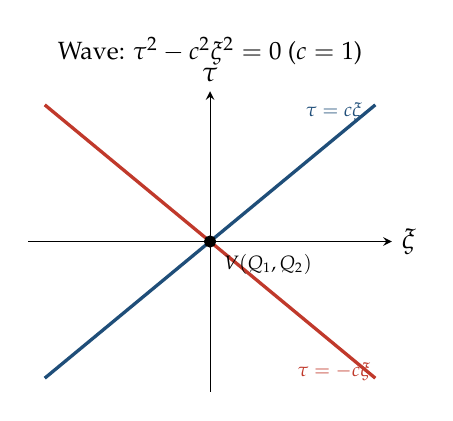
\begin{tikzpicture}
\begin{axis}[width=6.2cm,height=5.4cm,axis lines=middle,xlabel={$\xi$},ylabel={$\tau$},xmin=-2.2,xmax=2.2,ymin=-2.2,ymax=2.2,
 ticks=none,title={\small Wave: $\tau^2-c^2\xi^2=0$ ($c=1$)},every axis x label/.style={at={(current axis.right of origin)},anchor=west},
 every axis y label/.style={at={(current axis.above origin)},anchor=south}]
\addplot[cA,very thick,domain=-2:2] {x}; \addplot[cB,very thick,domain=-2:2] {-x};
\node[cA,font=\scriptsize] at (axis cs:1.5,1.9) {$\tau=c\xi$}; \node[cB,font=\scriptsize] at (axis cs:1.5,-1.9) {$\tau=-c\xi$};
\addplot[only marks,mark=*] coordinates {(0,0)}; \node[font=\scriptsize,anchor=north west] at (axis cs:0.05,-0.05) {$V(Q_1,Q_2)$};
\end{axis}
\end{tikzpicture}\hfill
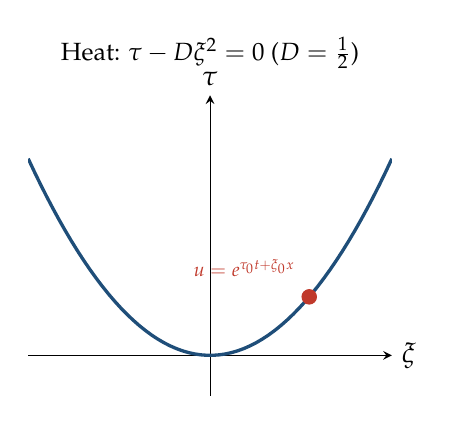
\begin{tikzpicture}
\begin{axis}[width=6.2cm,height=5.4cm,axis lines=middle,xlabel={$\xi$},ylabel={$\tau$},xmin=-2.2,xmax=2.2,ymin=-0.5,ymax=3.2,
 ticks=none,title={\small Heat: $\tau-D\xi^2=0$ ($D=\tfrac12$)},every axis x label/.style={at={(current axis.right of origin)},anchor=west},
 every axis y label/.style={at={(current axis.above origin)},anchor=south}]
\addplot[cA,very thick,domain=-2.2:2.2,samples=60] {0.5*x^2};
\addplot[only marks,mark=*,cB,mark size=2.6pt] coordinates {(1.2,0.72)};
\node[cB,font=\scriptsize,anchor=south east] at (axis cs:1.15,0.85) {$u=e^{\tau_0t+\xi_0x}$};
\end{axis}
\end{tikzpicture}
\caption{Real slices of characteristic varieties. A \emph{single exponential} corresponds to a single point of the variety; a rich, non-exponential solution ``fills'' the whole curve.}\label{fig:varieties}
\end{figure}

%--- E1: after Figure 1 (Section 2.1) ---------------------------------------
\begin{explained}{rings, the operator ring, symbol and characteristic variety}
\textbf{Step 0: what is a ring?} A \emph{ring} is the analogue of a group in which there are two operations, addition and multiplication. A set $R$ with $+$ and $\cdot$ is a ring if:
\begin{enumerate}[nosep]
\item $(R,+)$ is an abelian group: addition is associative and commutative, there is an additive identity $0$, and every element $a$ has an additive inverse $-a$;
\item multiplication is associative, $(ab)c=a(bc)$;
\item multiplication distributes over addition, $a(b+c)=ab+ac$ and $(a+b)c=ac+bc$.
\end{enumerate}
Unlike in a group, a ring does \emph{not} require every nonzero element to have a multiplicative inverse, and multiplication need not be commutative. The hierarchy is:
\begin{itemize}[nosep]
\item \emph{group}: one operation;
\item \emph{ring}: an additive abelian group together with a multiplication compatible with the addition;
\item \emph{field}: a commutative ring with $1\ne0$ in which every nonzero element has a multiplicative inverse.
\end{itemize}
Examples: $(\Z,+)$ is a group; $(\Z,+,\cdot)$ is a ring but not a field (2 has no inverse in $\Z$); $(\mathbb Q,+,\cdot)$ is a field. A ring is therefore \emph{not} simply a group under multiplication: it is an additive abelian group on which one can also multiply, with multiplication obeying the distributive law.

\medskip\textbf{Step 1: what is $\ring=\C[\partial_t,\partial_x]$?} It is the ring of polynomials in the two formal variables $\partial_t,\partial_x$ with complex coefficients. Elements of $\ring$ are, for instance,
\[
P(\partial)=\partial_t^2+\partial_x^2,\qquad Q(\partial)=3\partial_t\partial_x+2,\qquad S(\partial)=i\partial_t^3-5\partial_x .
\]
Why is it a ring? One can add operators ($P+Q$), multiply them by composing them ($PQ$), there is a zero operator and every operator has an additive inverse, and composition is associative and distributes over addition. The crucial point is that these are \emph{constant-coefficient} operators: the coefficients are complex numbers, not functions of $t$ or $x$. So $2\partial_t^2+3\partial_x+1$ is in $\ring$, whereas $t\,\partial_t$ is not (its coefficient $t$ is not constant).

\medskip\textbf{Step 2: why $\ring\cong\C[\tau,\xi]$?} The symbol $\cong$ means \emph{isomorphic}: the two rings have exactly the same algebraic structure. Here $\tau,\xi$ are ordinary formal polynomial variables and we simply replace
\[
\partial_t\longleftrightarrow\tau,\qquad\partial_x\longleftrightarrow\xi,
\qquad\text{e.g.}\qquad
\underbrace{\partial_t^2+3\partial_t\partial_x+2\partial_x^2}_{\text{differential operator}}\ \longleftrightarrow\ \underbrace{\tau^2+3\tau\xi+2\xi^2}_{\text{polynomial}} .
\]
This is legitimate because constant-coefficient partial derivatives commute, $\partial_t\partial_x=\partial_x\partial_t$, so the operator ring is commutative, exactly like the polynomial ring. At this stage $\tau$ and $\xi$ are \emph{not} numbers: they are formal variables that encode the operators.

\medskip\textbf{Step 3: the symbol.} For $P(\partial)=\partial_t^2-\partial_x^2+1$ the symbol is obtained by replacing each derivative with its variable,
\[
P(\tau,\xi)=\tau^2-\xi^2+1 .
\]
The symbol translates a differential operator into an algebraic object, and polynomial algebra is often easier to study than differential operators directly. \emph{Convention.} Other texts replace $\partial$ by $i\tau,i\xi$ (Fourier convention). In this paper the substitution is the \emph{direct} one, $\partial\mapsto(\tau,\xi)$; the Fourier convention $\partial_x\mapsto i\kappa$ appears only later, in Sections~\ref{sec:fact} and~\ref{sec:terms}, and is stated there.

\medskip\textbf{Step 4: the characteristic variety.} Given the symbol, $\Var(P)=\{(\tau,\xi)\in\C^2:P(\tau,\xi)=0\}$: the set of all pairs of complex numbers at which the symbol vanishes. For $P=\tau^2-\xi^2+1$ it is $\tau^2=\xi^2-1$, a subset of $\C^2$; a pair belongs to $\Var(P)$ exactly when it satisfies this equation. For $P=\tau-\xi$ it is the line $\tau=\xi$ of $\C^2$.

\medskip\textbf{Example: the wave operator.} $P(\partial)=\partial_t^2-c^2\partial_x^2$ has symbol $\tau^2-c^2\xi^2=(\tau-c\xi)(\tau+c\xi)$, so
\[
\Var(P)=\{\tau=c\xi\}\cup\{\tau=-c\xi\},
\]
two lines (Figure~\ref{fig:varieties}, left). They encode the characteristic directions of wave propagation; their precise interpretation depends on the PDE and on whether the covectors are taken real or complex.

\medskip\textbf{The whole passage in one picture.}
\[
\underbrace{P(\partial_t,\partial_x)}_{\text{operator on functions}}\ \xrightarrow{\ \partial\mapsto(\tau,\xi)\ }\ \underbrace{P(\tau,\xi)}_{\text{polynomial}}\ \xrightarrow{\ \text{zeros}\ }\ \underbrace{\Var(P)\subset\C^2}_{\text{set of points}}
\]
Three related but \emph{different} objects: an operator acting on functions, a polynomial, and a set of points of complex space.
\end{explained}



\subsection{Annihilators, ideals, and what a solution ``knows''}
A single $u$ is usually annihilated by many operators (the function $e^{x}$ is killed by $\partial_x-1$ and by $\partial_x^2-1$ and \dots).
\begin{definition}{(Annihilator)}\label{def:ann}
$\Ann(u)=\{Q\in\ring:\ Q(\partial)u=0\}$.
\end{definition}
(Readers new to ideals: see Appendix~\ref{app:primer}, \S B.1.) For instance $\Ann(e^{x})$ contains $\partial_x-1$ and its multiples such as $\partial_x^2-1=(\partial_x-1)(\partial_x+1)$. It is an \emph{ideal} of $\ring$: if $Qu=0$ and $S\in\ring$, then $(SQ)u=S(Qu)=0$; and sums of annihilators annihilate. Ideals are the polynomial analogue of the multiples of an integer: in one variable they are generated by a single polynomial, in two variables they may need several, and this is the source of all the subtleties below. We use three facts about $\C[\tau,\xi]$.
\begin{enumerate}[label=(F\arabic*),nosep]
\item \textbf{Unique factorization} (the polynomial analogue of prime factorization): $P=\prod_iP_i^{e_i}$ with $P_i$ irreducible (the ``primes'') and $e_i$ their multiplicities, unique up to constants; $\Gcd$ is defined as for integers. \\[1pt]\emph{Used for:} extracting the common part of an ideal (Lemma~\ref{lem:gcd}) and splitting an operator into factors (Section~\ref{sec:fact}).
\item \textbf{B\'ezout:} two polynomials in $\tau,\xi$ without common factor have only finitely many common zeros. \\[1pt]\emph{Geometrically:} two curves in $\C^2$ with no common component meet in isolated points. \\[1pt]\emph{Used for:} showing that what is left of an ideal after removing its gcd is ``small'' (Lemma~\ref{lem:gcd}).
\item \textbf{Nullstellensatz} (Hilbert): if $q$ vanishes on $\Var(I)$, the set of common zeros of all elements of the ideal $I$, then $q^k\in I$ for some $k$ (a power is needed because zeros do not see multiplicities). In particular an ideal without zeros is the whole ring. \\[1pt]\emph{Used for:} translating statements about zero sets into statements about ideals (proof of Theorem~\ref{thm:ident}, Proposition~\ref{prop:spec}).
\end{enumerate}
All three are classical~\cite{clo,fu}; they hold over $\C$, which is algebraically closed (the Nullstellensatz fails over $\R$).

\begin{notebox}{In the next lemma}
\begin{itemize}[nosep]
\item $\ring=\C[\tau,\xi]$ is the ring of Definition~\ref{def:ring};
\item $I\subset\ring$ is any ideal (in our use, $I=\Ann(u)$);
\item $g=\Gcd(I)$ is the polynomial of largest degree that divides every element of $I$, defined up to a nonzero constant;
\item $J=\{f/g:\ f\in I\}$ is the ideal of the quotients;
\item $\Var(J)\subset\C^2$ is the set of common zeros of all elements of $J$.
\end{itemize}
The lemma says that an ideal always splits into a ``curve part'' $g$ and a residue $J$ that vanishes only at finitely many points.
\end{notebox}
\begin{lemma}{(Splitting off the gcd) \led{C3-L2} \proved[]}\label{lem:gcd}
Every nonzero ideal $I\subset\ring$ factors as $I=g\cdot J$ with $g=\Gcd(I)$ and $\Var(J)$ finite.
\end{lemma}
\begin{proof}[Proof sketch]
Every $f\in I$ is divisible by $g$, so $J=\{f/g\}$ is well defined; it is again an ideal and $I=gJ$. The elements of $J$ have no common factor (a common factor $h$ would make $gh$ a common divisor of $I$).

Pick $0\ne h_1\in J$; if $h_1$ is constant, $J=\ring$ and $\Var(J)=\emptyset$. Otherwise let $p_1,\dots,p_r$ be its pairwise non-associate irreducible factors. For each $i$ there is $h_i'\in J$ with $p_i\nmid h_i'$ (otherwise $p_i$ would be a common factor). Put
\[
h_2=\sum_ih_i'\prod_{k\ne i}p_k\ \in J .
\]
Modulo $p_i$ only the $i$-th summand survives and it is not divisible by $p_i$, so no $p_i$ divides $h_2$: the two elements $h_1,h_2\in J$ have no common factor. By (F2) they have finitely many common zeros, and $\Var(J)\subseteq\Var(h_1,h_2)$ is finite.
\end{proof}

For $I=\Ann(u)$ we write $G_u=\Gcd\Ann(u)$ (defined up to a constant) and $J_u$ for the cofactor ideal: $\Ann(u)=G_u\,J_u$. Intuitively $G_u$ is the ``genuinely infinite-dimensional'' part of the equation of $u$, and $J_u$ the finitely many exponentials that happen to be present. These two objects drive Section~\ref{sec:ident}.

\begin{aside}{Two extreme examples}
\begin{itemize}[nosep]
\item For $u=e^{x}$, seen as a function of $(t,x)$, $\Ann(u)=(\tau,\ \xi-1)$ is the ideal of the single point $(0,1)$: $G_u=1$ and $J_u=\Ann(u)$, so $u$ has no infinite part.
\item For $u=f(x+t)$ with $f$ generic (not an exponential-polynomial), $\Ann(u)=(\tau-\xi)$: $G_u=\tau-\xi$ and $J_u=\ring$ (Section~\ref{sec:ident}).
\end{itemize}
\end{aside}

%--- E2: after Lemma 2.5 and the paragraph on G_u, J_u (Section 2.2) ---------
\begin{explained}{annihilators, ideals, (F1)--(F3) and the splitting of the gcd}
\textbf{Step 1: annihilating a function.} Take $u(x)=e^{x}$. Since $\partial_xe^x=e^x$, $(\partial_x-1)e^x=0$: the operator $\partial_x-1$ \emph{annihilates} $e^x$. It is not the only one: $(\partial_x^2-1)e^x=0$, and $\partial_x^2-1=(\partial_x-1)(\partial_x+1)$ is annihilating precisely because it contains the factor $\partial_x-1$. More generally, if $Q(\partial_x)e^x=0$ then every polynomial multiple of $Q$ annihilates $e^x$, for instance $(\partial_x+3)(\partial_x-1)e^x=0$. This is the basic reason annihilators are ideals.

\medskip\textbf{Step 2: the annihilator is the whole ideal $(\partial_x-1)$.} For $R=\C[\partial_x]$, any polynomial can be divided by $z-1$: $Q(z)=(z-1)S(z)+Q(1)$. Replacing $z$ by $\partial_x$ and applying to $e^x$ gives $Q(\partial_x)e^x=Q(1)e^x$, hence
\[
Q(\partial_x)e^x=0\iff Q(1)=0\iff(z-1)\mid Q(z).
\]
So $\Ann(e^x)=(\partial_x-1)=\{S(\partial_x)(\partial_x-1):S\in\C[\partial_x]\}$, and every annihilating polynomial is a multiple of $\partial_x-1$.

\medskip\textbf{Step 3: why an ideal.} An ideal is a subset closed under addition (and additive inverses) and under multiplication by any element of the ring. For annihilators: if $Qu=0$ and $Pu=0$ then $(Q+P)u=Qu+Pu=0$; if $Qu=0$ and $S\in\ring$ then $(SQ)u=S(Qu)=S(0)=0$. Intuition: once an operator kills a function, composing it with another constant-coefficient operator cannot bring the function back to life.

\medskip\textbf{Step 4: one variable versus two variables.} In $\C[\xi]$ every ideal is generated by a single polynomial, $I=(g)$ -- like the multiples of $6$ in $\Z$. In $\C[\tau,\xi]$ several generators may be needed. Consider $I=(\tau,\xi-1)=\{\tau A+(\xi-1)B\}$: neither generator is a multiple of the other and the ideal is not generated by one polynomial. This matters because the annihilator of a function of two variables can have several independent generators: for $u(t,x)=e^x$ we have $\partial_tu=0$ and $(\partial_x-1)u=0$, and
\[
\Ann(u)=(\partial_t,\ \partial_x-1).
\]
Both equations are needed to describe it in the two-variable ring.

\medskip\textbf{Step 5: the three facts.}
\begin{itemize}[nosep]
\item \textbf{(F1) Unique factorization.} Every nonzero polynomial factors into irreducibles, uniquely up to constants and order; e.g.\ $\tau^2-\xi^2=(\tau-\xi)(\tau+\xi)$. This allows one to define the gcd of an ideal: the greatest common polynomial factor of all its elements.
\item \textbf{(F2) B\'ezout.} Two polynomials in $(\tau,\xi)$ with no common nonconstant factor have finitely many common zeros in $\C^2$. Example: $\tau$ and $\xi-1$ have no common factor and their only common zero is $(0,1)$. Geometrically, two algebraic curves without a shared component meet in finitely many points.
\item \textbf{(F3) Nullstellensatz.} If $q$ vanishes on $\Var(I)$ then $q^k\in I$ for some $k\ge1$: $q|_{\Var(I)}=0\Rightarrow q^k\in I$. It connects the geometry of a zero set to the algebra of the ideal. The power matters: $q$ itself need not belong to $I$ (e.g.\ $I=(\tau^2)$, $q=\tau$).
\end{itemize}

\medskip\textbf{Step 6: the splitting lemma.} Every nonzero ideal $I\subset\ring$ can be written $I=gJ$, with $g=\Gcd(I)$ and $\Var(J)$ finite. Here $g$ is the polynomial factor shared by every element of $I$; $J$ is the ideal of the quotients $f/g$; because $g$ is the gcd, the elements of $J$ have no common nonconstant factor, and by (F2) their common zero set is finite. So the ideal splits into a common polynomial factor and a residual ideal with finite zero set.
\begin{itemize}[nosep]
\item \emph{Example A (shared factor).} $I=(\tau(\xi-1),\tau(\xi+1))$. Both generators contain $\tau$, so $g=\tau$ and $J=(\xi-1,\xi+1)$. Since $(\xi+1)-(\xi-1)=2$, $J=(1)=\ring$, whose zero set is empty (hence finite). Thus $I=(\tau)$.
\item \emph{Example B (no shared factor).} $I=(\tau,\xi-1)$: $g=1$, $J=I$, $\Var(J)=\{(0,1)\}$, finite.
\end{itemize}

\medskip\textbf{Step 7: applied to $u$.} Define $G_u=\Gcd\Ann(u)$ and call the remaining ideal $J_u$, so $\Ann(u)=G_uJ_u$. For $u=e^x$ in $\C[\partial_t,\partial_x]$ we found $\Ann(e^x)=(\partial_t,\partial_x-1)$; the generators have no common nonconstant factor, so
\[
G_u=1,\qquad J_u=(\partial_t,\partial_x-1),\qquad \Var(J_u)=\{(0,1)\},
\]
the single point corresponding to the exponential $e^{0\cdot t+1\cdot x}=e^x$. A point of the characteristic picture corresponds to a possible exponential mode. \emph{Qualification:} the reading of $G_u$ as the ``genuinely infinite-dimensional part'' and of $J_u$ as the ``finitely many exponentials present'' is an intuition for the later theory, not a universal identification for arbitrary functions without further hypotheses.
\end{explained}



\subsection{Exponential-polynomials}
\begin{notebox}{Notation used in this subsection}
\begin{itemize}[nosep]
\item Recall that $\ring=\C[\partial_t,\partial_x]\cong\C[\tau,\xi]$ (Definition~\ref{def:ring}) acts on functions by differentiation: $Q\in\ring$ sends $w$ to $Q(\partial)w$.
\item For a function $w$,
\[
\ring w=\spn\{\partial_t^j\partial_x^kw:\ j,k\ge0\}=\{Q(\partial)w:\ Q\in\ring\}
\]
is the set of all derivatives of $w$ and their linear combinations; it is a vector space over $\C$ and $\dimc_\C$ denotes its dimension as such.
\item The map $Q\mapsto Q(\partial)w$ from $\ring$ onto $\ring w$ has kernel $\Ann(w)$, which is why $\ring w\cong\ring/\Ann(w)$: the quotient identifies two operators that act in the same way on $w$.
\item In a sum $\sum_jp_j(t,x)e^{\tau_jt+\xi_jx}$, each $p_j$ is a polynomial in $(t,x)$ and each pair $(\tau_j,\xi_j)\in\C^2$ is an \emph{exponent}, i.e.\ a point of $\C^2$ as in Section~\ref{sec:prelim}.
\end{itemize}
\end{notebox}
\begin{definition}{(EP) \textcolor{cG}{\textsf{\footnotesize(see Appendix~\ref{app:primer}, \S B.2)}}}\label{def:ep}
$\EP$ is the set of finite sums $\sum_jp_j(t,x)\,e^{\tau_jt+\xi_jx}$ with polynomials $p_j$.
\end{definition}
\begin{lemma}{(Finite dimension criterion) \led{C3-L3} \proved[]}\label{lem:ep}
$w\in\EP\iff\dimc_\C(\ring w)<\infty$, where $\ring w=\spn\{\partial_t^j\partial_x^kw\}$ is the span of all derivatives of $w$. In that case $\ring w\cong\ring/\Ann(w)$ and $\Var(\Ann w)$ is the finite set of exponents $\{(\tau_j,\xi_j)\}$.
\end{lemma}
\begin{proof}[Idea of proof]
($\Rightarrow$) Derivatives of $p\,e^{\tau t+\xi x}$ are (polynomial of degree $\le\deg p$)$\,\cdot\,e^{\tau t+\xi x}$.
($\Leftarrow$) $\partial_t$ and $\partial_x$ act as commuting matrices on the finite-dimensional space $\ring w$. Commuting matrices are simultaneously triangularizable (the multivariable Jordan form); their joint eigenvalues are the exponents $(\tau_j,\xi_j)$, and the nilpotent parts produce the polynomial prefactors.
\end{proof}

\begin{takeaway}
Lemma~\ref{lem:ep} is the computational heart of the method: ``is $w$ an exponential-polynomial?'' is a \emph{finite-dimensional linear algebra question}. It is the test used in Theorem~\ref{thm:ident} and in Step~3 of the algorithm.
\end{takeaway}

%--- E3: after Lemma 2.7 (EP), before the Takeaway of Section 2.3 -----------
\begin{explained}{the finite dimension criterion for exponential-polynomials}
The lemma says: \emph{a function is a finite sum of polynomial-times-exponential terms if and only if all its derivatives span a finite-dimensional vector space.}

\medskip\textbf{Step 1: what is $\EP$?} The set of functions $w(t,x)=\sum_{j=1}^Np_j(t,x)e^{\tau_jt+\xi_jx}$, with $p_j$ polynomials and $\tau_j,\xi_j\in\C$. Examples: $e^{2t+x}+3e^{-t+4x}$ and $t^2e^x+(t+x)e^{t-x}$. The second has polynomial prefactors, so $\EP$ is more general than sums of pure exponentials. Polynomial prefactors appear because differentiating such a function gives another function of the same form: $\partial_x(te^{2t+x})=te^{2t+x}$ and $\partial_t(te^{2t+x})=(1+2t)e^{2t+x}$. The polynomial factor changes, the exponent stays the same.

\medskip\textbf{Step 2: what is $\ring w$?} $\ring w=\spn_\C\{\partial_t^j\partial_x^kw:j,k\ge0\}$, the vector space spanned by \emph{all} partial derivatives of $w$ (including $w$ itself): all finite complex linear combinations of them.
\begin{itemize}[nosep]
\item \emph{Pure exponential.} $w=e^{2t+3x}$: $\partial_t^j\partial_x^kw=2^j3^kw$, so $\ring w=\spn\{w\}$ and $\dim_\C\ring w=1$.
\item \emph{Polynomial times exponential.} $w=te^x$: $\partial_tw=e^x$, $\partial_t^2w=0$, $\partial_xw=te^x$; every higher derivative is a combination of $te^x$ and $e^x$, so $\ring w=\spn\{te^x,e^x\}$ and $\dim_\C\ring w=2$. Although $w$ has infinitely many derivatives, two independent functions span them all.
\end{itemize}

\medskip\textbf{Step 3 ($\Rightarrow$).} Let $f=p\,e^{\tau t+\xi x}$. Then $\partial_tf=(\partial_tp+\tau p)e^{\tau t+\xi x}$ and $\partial_xf=(\partial_xp+\xi p)e^{\tau t+\xi x}$. Differentiating a polynomial never raises its degree, so every derivative of $f$ is $q\,e^{\tau t+\xi x}$ with $\deg q\le\deg p$. The polynomials of degree $\le d$ in two variables form a space of dimension $(d+1)(d+2)/2$, so the derivatives of each term span a finite-dimensional space; $w$ has finitely many terms, so the same holds for $w$.

\medskip\textbf{Step 4 ($\Leftarrow$).} Suppose $W=\ring w$ is finite-dimensional. Differentiation maps derivatives to derivatives, so $\partial_tW\subseteq W$ and $\partial_xW\subseteq W$: they define linear operators $T=\partial_t|_W$ and $X=\partial_x|_W$. They commute ($TX=XT$, mixed partials commute). Commuting complex matrices are simultaneously triangularizable, so in a suitable basis both are upper triangular. Their diagonal entries give pairs of joint eigenvalues $(\tau_j,\xi_j)$; the joint generalized eigenspaces produce functions $p_j(t,x)e^{\tau_jt+\xi_jx}$: the diagonal part of differentiation produces the exponential, the nilpotent parts produce the polynomial factors (they vanish when raised to a high enough power, since the space is finite-dimensional). There are finitely many pairs, hence $w\in\EP$.

\medskip\textbf{Step 5: $\ring w\cong\ring/\Ann(w)$.} Define $\Phi:\ring\to\ring w$, $Q\mapsto Qw$. It is surjective (by definition of $\ring w$) and its kernel is exactly $\Ann(w)$ (since $\Phi(Q)=0$ means $Qw=0$). By the first isomorphism theorem $\ring w\cong\ring/\Ann(w)$. The quotient identifies two operators exactly when they act identically on $w$: $P\sim Q\iff(P-Q)w=0$. Hence
\[
w\in\EP\iff\dim_\C\ring/\Ann(w)<\infty .
\]

\medskip\textbf{Step 6: $\Var(\Ann w)$ is the set of exponents.} For $w=te^x$, $\Ann(w)=(\partial_t^2,\partial_x-1)$, with symbol ideal $(\tau^2,\xi-1)$. Its zero set is $\{\tau^2=0,\ \xi=1\}=\{(0,1)\}$ (over $\C$, $\tau^2=0$ forces $\tau=0$), exactly the exponent pair of $te^{0t+1x}$. For a general exponential-polynomial the variety gives the \emph{distinct} exponent pairs that occur. It does \emph{not} record multiplicities or the full polynomial prefactors: those affect the structure of the annihilator but introduce no new exponent pairs.

\medskip\textbf{Step 7: why it is computationally important.} The criterion converts a question about the \emph{form} of a function into finite-dimensional linear algebra. If one can establish relations such as $\partial_t^2w=2\partial_tw+w$ and $\partial_xw=3w$, then every mixed derivative reduces to a combination of $w$ and $\partial_tw$, so $\dim\ring w\le2$ and $w\in\EP$. The big picture: the annihilator encodes all differential equations satisfied by $w$; the quotient $\ring/\Ann(w)$ counts the independent derivatives; the joint eigenvalues of differentiation identify the exponential modes.
\end{explained}


%======================================================================
\section{One variable: the ODE prototype}\label{sec:ode}
\sectionbrief
{one variable $x$, an ODE $p(D)u=0$ with constant coefficients, $D=d/dx$, $p$ known.}
{in one variable every object of the later sections (minimal annihilator, spectral projectors, companion matrix) appears with explicit formulas and no geometry of curves.}
{prototype for Section~\ref{sec:ident} (identification) and Section~\ref{sec:fact} (the Lagrange projectors reappear as Eq.~\eqref{eq:lagrange}).}
This section introduces, in the simplest setting, objects that reappear in Sections~\ref{sec:ident} and~\ref{sec:fact}: the minimal annihilator, the companion matrix and the spectral projectors.

\begin{notebox}{Setting and symbols}
\begin{itemize}[nosep]
\item We consider an ODE $p(D)u=0$ in one variable $x$, with $D=d/dx$ (in this section only; elsewhere $D$ is a diffusion constant).
\item The polynomial $p(\lambda)=\prod_j(\lambda-\lambda_j)^{m_j}$ has distinct roots $\lambda_j\in\C$ with multiplicities $m_j\ge1$, so that $m=\deg p=\sum_jm_j$ is the \emph{order} of the equation (not to be confused with the Sobolev index $m$ of Section~\ref{sec:fact}).
\item The set of solutions is the \emph{kernel} $\ker p(D)$, and
\[
\ker p(D)=\Big\{\sum_jq_j(x)e^{\lambda_jx}:\ \deg q_j<m_j\Big\},
\]
where each $q_j$ is a polynomial of degree $<m_j$.
\end{itemize}
\end{notebox}

\begin{aside}{Why this form}
For one root, $(D-\lambda)\big(q\,e^{\lambda x}\big)=q'e^{\lambda x}$: applying $D-\lambda$ lowers the degree of $q$ by one. Hence $(D-\lambda_j)^{m_j}$ kills $q\,e^{\lambda_jx}$ exactly when $q^{(m_j)}=0$, i.e.\ $\deg q<m_j$.

Each root therefore contributes the $m_j$ functions $x^ke^{\lambda_jx}$ ($0\le k<m_j$): these are the natural basis functions of the equation, finitely many, and together they form a basis of $\ker p(D)$, a space of dimension $m$.
\end{aside}

\begin{aside}{Example}
$p(\lambda)=(\lambda-1)^2(\lambda+2)^3$ has $\lambda_1=1$, $m_1=2$, $\lambda_2=-2$, $m_2=3$, order $m=5$. A basis of the solutions is
\[
e^{x},\quad xe^{x},\quad e^{-2x},\quad xe^{-2x},\quad x^2e^{-2x},
\]
so every solution is
\[
c_1e^{x}+c_2xe^{x}+c_3e^{-2x}+c_4xe^{-2x}+c_5x^2e^{-2x}.
\]
\end{aside}

\subsection{Identification by the Wronskian}
\begin{proposition}{(ODE identification)}
Let $u\in\ker p(D)$. The minimal annihilator of $u$ has degree equal to the number of independent basis functions actually present in $u$; it equals $p$ if and only if $u,u',\dots,u^{(m-1)}$ are linearly independent (nonvanishing Wronskian), i.e.\ iff every root of $p$ appears in $u$ with its full multiplicity.
\end{proposition}
\emph{Reason.} $\dimc\spn\{u,u',u'',\dots\}$ is the degree of the minimal annihilator (Lemma~\ref{lem:ep} in one variable); a missing root lowers it.

\subsection{The companion matrix and spectral form}
Write $p(\lambda)=\lambda^m+a_{m-1}\lambda^{m-1}+\dots+a_0$ (monic) and put $X=(u,u',\dots,u^{(m-1)})^{\top}$. Then $X'=CX$ with
\[
C=\begin{pmatrix}0&1&&\\&0&\ddots&\\&&\ddots&1\\-a_0&-a_1&\cdots&-a_{m-1}\end{pmatrix},\qquad
X(x)=e^{xC}X(0).
\]
The eigenvalues of $C$ are the roots of $p$. For distinct roots the matrix exponential has the spectral form
\begin{equation}\label{eq:spectral}
\begin{aligned}
e^{xC}&=\sum_{j=1}^me^{\lambda_jx}\,\Pi_j,\\
\Pi_j&=\prod_{k\ne j}\frac{C-\lambda_k\Id}{\lambda_j-\lambda_k},
\end{aligned}
\end{equation}
where the $\Pi_j$ are the Lagrange projectors onto the eigenspaces. The last row of $C$ carries the whole equation; $C$ is a \emph{matrix over the base field} for an ODE, but, as soon as the coefficients depend on $x$, or there is a second variable, its last row has entries that are operators and the object becomes a matrix over a noncommutative or polynomial ring. The invariant statement is that the whole equation corresponds to the cyclic module $\ring/\Ann(u)$ (Section~\ref{sec:prelim}); the companion matrix is a way to compute with it relative to one chosen direction.

\begin{proposition}{(Projectors of the companion matrix) \led{II-T2} \proved[]}
The projectors $\Pi_j$ are explicit rational functions of the coefficients, with poles exactly where roots collide; they are polynomial in the coefficients if and only if the corresponding varieties are disjoint. They are \emph{not} orthogonal in general: the companion matrix is not normal for $m=2$ \falsest{} (the contrary was an early conjecture).
\end{proposition}
Hence Hilbert-space orthogonality arguments need an inner product adapted to the problem, not the standard one on the coefficient vector.

\subsection{Tensor construction versus module construction}
One may encode a PDE in a higher-order tensor of derivatives, $J=\partial_{x_{i_1}}\otimes\cdots\otimes\partial_{x_{i_n}}$, or by the companion form. The comparison, \led{Gate 3}: the \emph{principal symbol tensor} $\sigma_m(P)\in\mathrm{Sym}^m(\C^2)$ only sees the highest-order part of $P$ (for the heat operator it sees $\xi^2$ alone), so it is an invariant ``at infinity''; the \emph{cyclic module} $\ring/\Ann(u)$ is the complete invariant. All subsequent results use the module.

%--- E4: end of Section 3, before the keypoint ------------------------------
\begin{explained}{the ODE prototype, step by step}
This section is the one-dimensional version of the whole theory. It starts with an ODE because in one variable the algebra is completely explicit: roots of a polynomial determine the solutions, and the roots lead naturally to the minimal annihilator, the companion matrix and the spectral projectors.

\medskip\textbf{Step 1: the ODE.} $p(D)u=0$ with $D=d/dx$ and $p$ of degree $m$, factored over $\C$ as $p(\lambda)=\prod_{j=1}^r(\lambda-\lambda_j)^{m_j}$, $\sum_jm_j=m$: the $\lambda_j$ are the distinct roots, $m_j$ their multiplicities, $m$ the total degree. For $p(\lambda)=(\lambda-1)^2(\lambda+2)^3$ the equation $(D-1)^2(D+2)^3u=0$ has order five.

\medskip\textbf{Step 2: why solutions are $q(x)e^{\lambda x}$.} First, $(D-\lambda)e^{\lambda x}=0$. If the root has multiplicity greater than one, further solutions appear: $(D-\lambda)(xe^{\lambda x})=e^{\lambda x}$, hence $(D-\lambda)^2(xe^{\lambda x})=0$; in general $(D-\lambda)^m(x^ke^{\lambda x})=0$ for $0\le k<m$. The reason is the identity
\[
(D-\lambda)\big(q(x)e^{\lambda x}\big)=q'(x)e^{\lambda x}:
\]
each application of $D-\lambda$ differentiates the polynomial prefactor once, and after $m$ applications a polynomial of degree $<m$ has vanished. A root of multiplicity $m_j$ therefore contributes the $m_j$ solutions $e^{\lambda_jx},xe^{\lambda_jx},\dots,x^{m_j-1}e^{\lambda_jx}$, and the complete solution space is
\[
\ker p(D)=\Big\{\sum_{j=1}^rq_j(x)e^{\lambda_jx}:\deg q_j<m_j\Big\}.
\]
\emph{Worked example.} For $(\lambda-1)^2(\lambda+2)^3$: root $1$ (multiplicity 2) gives $e^x,xe^x$; root $-2$ (multiplicity 3) gives $e^{-2x},xe^{-2x},x^2e^{-2x}$. Five independent solutions, so the solution space has dimension five $=m$: the number of natural basis functions is finite and equals the degree of $p$.

\medskip\textbf{Step 3: the minimal annihilator.} For a particular function $u$, $\Ann(u)=\{Q\in\C[D]:Q(D)u=0\}$. In one variable the annihilator of a nonzero $u$ is generated by a single polynomial of smallest degree; normalized to be monic it is the \emph{minimal annihilating polynomial} of $u$. Example: $u=xe^x$ has $(D-1)u=e^x$ and $(D-1)^2u=0$, so its minimal annihilator is $p_u(D)=(D-1)^2$; the multiplicity two tells that the solution has a polynomial prefactor of degree one. The polynomial $p$ defining the ODE need not be minimal for a particular solution: $u=e^x$ solves $(D-1)^2u=0$, but its minimal annihilator is only $D-1$.

\medskip\textbf{Step 4: the companion matrix.} Write $p(\lambda)=\lambda^m+a_{m-1}\lambda^{m-1}+\dots+a_0$. Then $u^{(m)}=-a_{m-1}u^{(m-1)}-\dots-a_0u$. With the state vector $Y=(u,u',\dots,u^{(m-1)})^\top$ the ODE becomes $Y'=CY$, with $C$ the companion matrix displayed in the text. Its characteristic polynomial is $p(\lambda)$: the roots of the polynomial become the eigenvalues of a matrix, and the multiplicities determine the possible Jordan blocks.

\medskip\textbf{Step 5: spectral projectors.} Suppose first the roots are distinct. The Lagrange polynomials $\ell_j(z)=\prod_{k\ne j}\frac{z-\lambda_k}{\lambda_j-\lambda_k}$ satisfy $\ell_j(\lambda_i)=1$ if $i=j$ and $0$ if $i\ne j$. Substituting the matrix gives the projectors $\Pi_j=\ell_j(C)$; each projects onto the eigenspace of $\lambda_j$, and $\Pi_i\Pi_j=0$ for $i\ne j$, $\sum_j\Pi_j=\Id$. Consequently $e^{xC}=\sum_je^{\lambda_jx}\Pi_j$ when $C$ is diagonalizable with distinct eigenvalues. When roots are repeated, eigenspace projectors alone do not capture the polynomial factors: one needs the generalized eigenspaces and the nilpotent parts of the Jordan blocks, which produce $xe^{\lambda x}$, $x^2e^{\lambda x}$, \dots

\medskip\textbf{Step 6: why this is the prototype.}
\begin{center}\small
\begin{tabular}{@{}L{5.6cm}L{8.6cm}@{}}
\toprule
One-dimensional ODE & Later multivariable theory\\\midrule
polynomial $p(\lambda)$ & polynomial symbol $P(\tau,\xi)$\\
roots $\lambda_j$ & exponent pairs $(\tau_j,\xi_j)$\\
minimal annihilating polynomial & annihilator ideal and its gcd\\
companion matrix & commuting differentiation operators on a finite-dimensional space\\
Lagrange spectral projectors & projectors isolating the individual exponential modes\\
\bottomrule
\end{tabular}
\end{center}
In one variable the roots are isolated points and polynomial factorization gives the whole picture. In two variables the common zero set of polynomials can contain entire curves, so the geometry and the ideal decomposition become more subtle.
\end{explained}



\begin{keypoint}
This section shows how an ODE's polynomial encodes its solution space. Its roots determine the exponential rates, their multiplicities determine the polynomial prefactors, the companion matrix represents differentiation, and spectral projectors isolate the different modes. The later sections generalize these ideas to multiple commuting derivatives, where the same structure survives but requires more algebraic machinery: the minimal annihilator becomes the ideal $\Ann(u)$ (Section~\ref{sec:ident}) and the Lagrange projectors reappear as Eq.~\eqref{eq:lagrange} (Section~\ref{sec:fact}).
\end{keypoint}

%======================================================================
\section{Identification}\label{sec:ident}
\sectionbrief
{$\Omega\subset\R^2$ open and connected, $u\in\mathcal D'(\Omega)$, constant coefficients, and an operator $P$ with $P(\partial)u=0$ is available (any annihilator).}
{to decide whether $u$ pins down the equation it solves, i.e.\ whether $P$ can be recovered from $u$ alone.}
{first link of the chain in Figure~\ref{fig:pipeline}: it defines $G_u$ and the test ``$\in\EP$'' that Sections~\ref{sec:fact} and~\ref{sec:algo} reuse. \emph{Result:} a necessary and sufficient criterion (Theorem~\ref{thm:ident}) and its limits.}

\subsection{The main criterion}
Let $\Omega\subset\R^2$ be open and \emph{connected} (connectedness is necessary: on disconnected $\Omega$ different components can satisfy different equations), $u\in\mathcal D'(\Omega)$ with $P(\partial)u=0$ and $P=\prod_iP_i^{e_i}$ the irreducible factorization.

\begin{notebox}{Terminology}
\begin{itemize}[nosep]
\item $\EP(\Omega)$ denotes the restrictions to $\Omega$ of exponential-polynomials (Definition~\ref{def:ep}).
\item $P$ is \emph{reduced} if all $e_i=1$ (no repeated factor).
\item $P$ is \emph{monic in $\tau$} if, written as a polynomial in $\tau$ with coefficients in $\C[\xi]$, its leading coefficient is a nonzero constant; then $k=\deg_\tau P$ is its order in time and the \emph{$t$-jet} of $u$ is the vector $(u,\partial_tu,\dots,\partial_t^{k-1}u)$.
\item In (a) we remove one copy of $P_i$ from $P$; in (b) we remove the whole power $P_i^{e_i}$, which makes (b) sensitive to multiplicities.
\end{itemize}
\end{notebox}
\begin{theorem}{(Identification criterion) \led{C3-T1} \proved[]}\label{thm:ident}
\begin{enumerate}[label=(\alph*),leftmargin=*,nosep]
\item $\displaystyle\Ann(u)=(P)\iff\Big(\frac{P}{P_i}\Big)(\partial)\,u\notin\EP(\Omega)\ \text{ for every irreducible factor }P_i\text{ of }P.$
\item $\Var(\Ann u)=\Var(P)$ iff $(P/P_i^{e_i})(\partial)u\notin\EP$ for all $i$.
\item For $P$ reduced the statements (a) and (b) coincide; for $P$ monic in $\tau$ the test can be carried out on the $t$-jet $u,\partial_tu,\dots,\partial_t^{k-1}u$ \led{II-C1}.
\end{enumerate}
\end{theorem}
\begin{intuition}
Strip one irreducible factor off $P$ and look at what is left: $w_i=(P/P_i)(\partial)u$ lies in $\ker P_i$. If $w_i$ is a ``generic'' member of that kernel (not a finite sum of exponentials), then no smaller operator can kill $u$. If $w_i$ is an exponential-polynomial, $u$ contains a finite-dimensional piece that is also killed by an operator of lower order, and $u$ cannot tell the large equation from the small one.
\end{intuition}
\begin{proposition}{(Uniqueness of the identified operator)}\label{prop:unique}
If $\Ann(u)=(P)$, then $P$ is determined by $u$ up to a nonzero constant factor: every constant-coefficient operator $Q$ with $Q(\partial)u=0$ is a multiple $Q=SP$ with $S\in\ring$, and $P$ is, up to a constant, the \emph{only} annihilator of minimal degree. If instead $\Ann(u)\supsetneq(P)$, the equation is \emph{not} identified: $P$ cannot be recovered from $u$, and the only object intrinsic to $u$ is the generator $G_u$ of the infinite part of $\Ann(u)$ (Section~\ref{sec:spectral}).
\end{proposition}
\begin{proof}
$Q\in(P)$ means $Q=SP$ for some $S\in\ring$, which is the first claim. Since degrees add, $\deg Q=\deg S+\deg P\ge\deg P$ for $Q\ne0$, with equality iff $S$ is constant. Two generators of the same principal ideal differ by a unit of $\ring$, i.e.\ by a nonzero constant.
\end{proof}

\begin{example}[Heat equation]\label{ex:heat}
Take $P=\tau-D\xi^2$ with $D>0$, i.e.\ $u_t=Du_{xx}$. $P$ is irreducible, so $P/P_i=1$ and the criterion reads: $\Ann(u)=(P)$ iff $u\notin\EP$. Three cases show what this means.
\begin{enumerate}[label=(\roman*),nosep]
\item \emph{One Fourier mode.} Let $u=e^{-D\kappa^2t+i\kappa x}$ with $\kappa\in\R$ fixed. Then $u_t=-D\kappa^2u$ and $u_{xx}=-\kappa^2u$, so $P(\partial)u=0$. But also $(\partial_x-i\kappa)u=0$ and $(\partial_t+D\kappa^2)u=0$, so
\[
\Ann(u)=(\tau+D\kappa^2,\ \xi-i\kappa),
\]
the maximal ideal of the point $(-D\kappa^2,i\kappa)$ of $\Var(P)$. It is strictly larger than $(P)$; indeed
\[
P=(\tau+D\kappa^2)-D\,(\xi-i\kappa)(\xi+i\kappa)\in\Ann(u).
\]
\item \emph{A finite superposition of modes.} Let $u=\sum_{j=1}^rc_je^{-D\kappa_j^2t+i\kappa_jx}$ with distinct $\kappa_j$ and $c_j\ne0$. Then $u\in\EP$, so $\Ann(u)\ne(P)$: it is the ideal of the $r$ points $(-D\kappa_j^2,i\kappa_j)$, and contains many operators that are not multiples of $P$.
\item \emph{The heat kernel.} Let $u=t^{-1/2}e^{-x^2/(4Dt)}$ for $t>0$ (up to the normalizing constant $(4\pi D)^{-1/2}$). Its $x$-derivatives are polynomials of growing degree times the same Gaussian, so they span an infinite-dimensional space and $u\notin\EP$ (Lemma~\ref{lem:ep}). By the criterion $\Ann(u)=(P)$, and by Proposition~\ref{prop:unique} every constant-coefficient equation satisfied by the heat kernel is a multiple of $\tau-D\xi^2$.
\end{enumerate}
\emph{Message.} A ``poor'' solution (in $\EP$) remembers only finitely many exponentials and cannot tell the heat equation from many others; a ``rich'' solution (outside $\EP$) remembers the whole equation.
\end{example}

\begin{proof}[Proof of the easy direction of (a): $\Rightarrow$, by contraposition]
Suppose $w_i\in\EP$ for some $i$.
\begin{enumerate}[nosep,label=\arabic*.]
\item By Lemma~\ref{lem:ep}, $J=\Ann(w_i)$ has a finite zero set.
\item Since $\Var(P_i)$ is a curve (infinite), it contains a point at which some $q\in J$ does not vanish; hence $q$ does not vanish identically on $\Var(P_i)$, and by (F3) $P_i\nmid q$ (if $P_i\mid q$ then $q$ would vanish on $\Var(P_i)$; conversely if $q$ vanished there, $q^k\in(P_i)$ and, $P_i$ being irreducible, $P_i\mid q$).
\item Then $(P/P_i)\,q\in\Ann(u)$ because $(P/P_i)q\,u=q\,w_i=0$;
\item but $(P/P_i)q\notin(P)$, since divisibility by $P$ would force $P_i\mid q$.
\end{enumerate}
So $\Ann(u)\supsetneq(P)$. \end{proof}
The converse uses the structure of ideals (Lemma~\ref{lem:gcd}) and the Nullstellensatz, and is given in the project's proof package\edmark{E6}.

%--- E5: Section 4.1, after the easy-direction proof / before the takeaway --
\begin{explained}{what Theorem~\ref{thm:ident} asks, and why}
\textbf{Step 1: the problem.} Given an open connected $\Omega\subset\R^2$, a distribution $u\in\mathcal D'(\Omega)$ and a constant-coefficient operator with $P(\partial)u=0$, does $u$ \emph{uniquely identify} $P$, in the sense $\Ann(u)=(P)$? That equality says that every constant-coefficient operator annihilating $u$ is a multiple of $P$: there is no genuinely smaller equation. A single function can satisfy many different PDEs, so the answer is not automatically yes.

\medskip\textbf{Counterexample.} $P=\partial_x^2-1=(\partial_x-1)(\partial_x+1)$ and $u=e^x$: $P(\partial)u=0$, but also $(\partial_x-1)u=0$, so $\Ann(u)\ne(P)$ (in $\C[\partial_x]$ it equals $(\partial_x-1)$; in $\ring$ it is $(\partial_t,\partial_x-1)$). Knowing $u=e^x$ does not tell us that the second-order equation is the minimal one.

\medskip\textbf{Step 2: factor $P$.} $P=\prod_{i=1}^rP_i^{e_i}$ with distinct irreducible $P_i$. Example: $P=(\tau-\xi)^2(\tau+\xi)$ has $P_1=\tau-\xi$ ($e_1=2$) and $P_2=\tau+\xi$ ($e_2=1$). Each factor is a potential piece of the equation that might be unnecessary to explain this particular $u$.

\medskip\textbf{Step 3: the key construction.} For each $i$ put $w_i=(P/P_i)(\partial)u$. Because $P(\partial)u=0$,
\[
P_i(\partial)w_i=P_i(\partial)\tfrac{P}{P_i}(\partial)u=P(\partial)u=0,\qquad\text{i.e.}\qquad w_i\in\ker P_i(\partial).
\]
After removing one factor, the resulting function satisfies the PDE of that factor alone. The theorem asks whether $w_i$ is an exponential-polynomial:
\begin{itemize}[nosep]
\item $w_i\notin\EP$: it has infinitely many independent derivatives, which prevents the factor $P_i$ from being removed from the annihilator;
\item $w_i\in\EP$: it lives in a finite-dimensional derivative space, which signals a possible ambiguity in identifying the equation.
\end{itemize}

\medskip\textbf{Step 4: part (a).} $\Ann(u)=(P)\iff(P/P_i)(\partial)u\notin\EP(\Omega)$ for every $i$. If another annihilator $Q$ were not a multiple of $P$, the annihilator would contain more information than $(P)$; the theorem rules this out precisely by the non-$\EP$ tests. \emph{Check on the counterexample:} for $P_1=\partial_x-1$, $P/P_1=\partial_x+1$ and $w_1=(\partial_x+1)e^x=2e^x\in\EP$; for $P_2=\partial_x+1$, $w_2=(\partial_x-1)e^x=0\in\EP$. The tests say $\EP$, so $u$ does not identify $P$, as it should. Note the theorem concerns the \emph{full annihilator ideal}, not merely whether $P$ is satisfied.

\medskip\textbf{Step 5: part (b).} $\Var(\Ann u)=\Var(P)\iff(P/P_i^{e_i})(\partial)u\notin\EP$ for all $i$. In (a) one removes one copy of $P_i$, in (b) the whole power $P_i^{e_i}$, because the characteristic variety sees zeros, not multiplicities. For instance $(\tau-\xi)^2$ and $\tau-\xi$ have the same zero set $\{\tau=\xi\}$ but are different polynomials. Identifying the variety is therefore weaker than identifying the annihilator.

\medskip\textbf{Step 6: part (c).} If $P$ is \emph{reduced} (all $e_i=1$), removing one copy of $P_i$ equals removing its whole power, so (a) and (b) coincide. If $P$ is monic in $\tau$ of degree $k$ in $\tau$, the test can be done on the finite $t$-jet $u,\partial_tu,\dots,\partial_t^{k-1}u$: a jet is just a finite list of derivatives, so the test needs only finitely many derivative components.

\medskip\textbf{The logical chain.} Given $P(\partial)u=0$ $\to$ factor $P$ $\to$ remove factors, $w_i=(P/P_i)(\partial)u$ $\to$ test membership in $\EP$ (finite-dimensional derivative span, Lemma~\ref{lem:ep}) $\to$ decide whether $u$ determines the full annihilator or only its characteristic variety. One precision: the theorem does \emph{not} say that an exponential-polynomial solution can never identify any PDE; it tests the particular functions $w_i$ obtained after removing factors, not whether $u$ itself is in $\EP$.
\end{explained}



\begin{takeaway}
Theorem~\ref{thm:ident} turns ``does $u$ identify $P$?'' into finitely many membership tests ``$\in\EP$'', each a finite-dimensional computation (Lemma~\ref{lem:ep}). What remains unsettled is whether those tests can actually be carried out from the data one has; this is the subject of Section~\ref{sec:ident-limits}.
\end{takeaway}



\subsection{The spectral form}\label{sec:spectral}
Theorem~\ref{thm:ident} says when $(P)$ is the whole annihilator. Proposition~\ref{prop:spec} restates this through the two pieces of $\Ann(u)$ given by Lemma~\ref{lem:gcd}.

\begin{notebox}{Notation}
\begin{itemize}[nosep]
\item $G_u=\Gcd\Ann(u)$ is the ``infinite part'' of $\Ann(u)$, $J_u$ is the cofactor ($\Ann(u)=G_uJ_u$), and
\[
\sigma_p(u)=\Var(J_u)\subset\C^2
\]
is the \emph{point spectrum} of $u$: a finite set of exponents $(\tau_0,\xi_0)$, i.e.\ of exponentials $e^{\tau_0t+\xi_0x}$ that are ``present'' in $u$. (``Spectrum'' is used in an algebraic sense, not as the spectrum of an operator on a Hilbert space.)
\item We write $G_u\sim P$ when $G_u$ and $P$ agree up to a nonzero constant factor.
\end{itemize}
\end{notebox}
\begin{proposition}{(Spectral characterization) \led{P4-T2} \proved[]}\label{prop:spec}
Let $P$ be an annihilator of $u$. Then
\[
\Ann(u)=(P)\iff \sigma_p(u)=\emptyset\ \text{ and }\ G_u\sim P .
\]
Further $\ring u\cap\EP\cong\ring/J_u$.
\end{proposition}
\begin{proof}[Derivation of the equivalence]
$(\Rightarrow)$ If $\Ann(u)=(P)$, the gcd of the ideal is $P$, so $G_u\sim P$ and $J_u=\ring$; then $\sigma_p(u)=\Var(\ring)=\emptyset$.

$(\Leftarrow)$ If $\sigma_p(u)=\Var(J_u)=\emptyset$, the Nullstellensatz (F3) gives $1\in J_u$, i.e.\ $J_u=\ring$, hence $\Ann(u)=G_u\ring=(G_u)=(P)$ because $G_u\sim P$.

The isomorphism $\ring u\cap\EP\cong\ring/J_u$ is not rederived here: it follows from $\ring u\cong\ring/\Ann(u)$ (Lemma~\ref{lem:ep}) by passing to the finite-dimensional part (ledger P4-T2)\edmark{E11}.
\end{proof}
\emph{Illustration.} For $u=e^{\tau_0t+\xi_0x}$ one has $\Ann(u)=(\tau-\tau_0,\xi-\xi_0)$, so $G_u=1$ and $\sigma_p(u)=\{(\tau_0,\xi_0)\}$: a single exponential has no ``infinite part'' and a one-point spectrum. For $u=e^{\tau_1t+\xi_1x}+e^{\tau_2t+\xi_2x}$ with distinct exponents, $G_u=1$ and $\sigma_p(u)$ has two points. For a solution of $P(\partial)u=0$ with $\Ann(u)=(P)$ one has $\sigma_p(u)=\emptyset$ and $G_u\sim P$.

\begin{aside}{What $G_u$ is good for}
Thus $G_u$ is the correct ``operator intrinsic to $u$'': it depends only on $u$, whereas $P$ depends on which annihilator was chosen. It is recovered from \emph{any} annihilator $P$ by at most $\sum_ie_i$ membership tests ``$\in\EP$'' \led{C3-T6} (one test for each copy of an irreducible factor that may have to be dropped; see Step~4 of the algorithm).
\end{aside}

\begin{aside}{Why $G_u$ and not the full variety}
A tempting stronger formulation replaces $G_u$ by the variety $\Var(\Ann u)$. It is correct only for reduced $P$, because zero sets do not see multiplicities.

\emph{Example:} $P=\tau^2$ and $u=e^{x^2}$. Then $P(\partial)u=u_{tt}=0$. Since $\partial_x^ke^{x^2}$ is a polynomial of degree exactly $k$ times $e^{x^2}$, no nonzero polynomial in $\partial_x$ alone kills $u$, hence
\[
\Ann(u)=(\tau).
\]
Here $\sigma_p(u)=\emptyset$ but $G_u=\tau\not\sim P$, so $\Ann(u)\ne(P)$, while $\Var(\Ann u)=\{\tau=0\}=\Var(P)$: the variety criterion would wrongly say that $u$ identifies $\tau^2$\edmark{E12}.
\end{aside}

%--- E6: Section 4.2, after the aside "Why G_u and not the full variety" -----
\begin{explained}{the point spectrum and the intrinsic operator $G_u$}
\textbf{Step 1: the decomposition.} By Lemma~\ref{lem:gcd}, $\Ann(u)=G_uJ_u$ with $G_u=\Gcd\Ann(u)$ and $\Var(J_u)$ finite. $G_u$ captures the common polynomial factor of all annihilating equations; $J_u$ captures the residual finite structure. The paper calls $\sigma_p(u)=\Var(J_u)$ the \emph{point spectrum} of $u$: a point $(\tau_0,\xi_0)$ corresponds to the exponential $e^{\tau_0t+\xi_0x}$. ``Spectrum'' is used in an algebraic sense: a finite set of exponent pairs, not a set of Fourier frequencies.

\medskip\textbf{Step 2: why $\Ann(u)=(P)\iff\sigma_p(u)=\emptyset$ and $G_u\sim P$.} Here $G_u\sim P$ means they differ by a nonzero constant.
\begin{itemize}[nosep]
\item Suppose $\sigma_p(u)=\emptyset$, i.e.\ $\Var(J_u)=\emptyset$. Over $\C$ the Nullstellensatz says an ideal without common zeros is the whole ring, so $J_u=\ring$ and $\Ann(u)=G_u\ring=(G_u)$: with empty point spectrum the annihilator is generated by its gcd. If moreover $G_u\sim P$, then $\Ann(u)=(P)$.
\item Conversely if $\Ann(u)=(P)$, the gcd is $P$ up to a constant, the cofactor ideal is $\ring$ and its zero set is empty.
\end{itemize}
Interpretation: the equation is fully identifiable when there is no residual finite point spectrum and the common gcd agrees with the proposed operator.

\medskip\textbf{Step 3: a single exponential.} $u=e^{\tau_0t+\xi_0x}$ has $\partial_tu=\tau_0u$, $\partial_xu=\xi_0u$, so $\Ann(u)=(\tau-\tau_0,\xi-\xi_0)$. The generators have no common nonconstant factor: $G_u=1$, $J_u=(\tau-\tau_0,\xi-\xi_0)$, and
\[
\sigma_p(u)=\{(\tau_0,\xi_0)\}:
\]
one point, exactly the exponential in $u$. Since $G_u=1$ and the spectrum is nonempty, this $u$ does not identify any nonconstant operator as the generator of its full annihilator: $\partial_t-\tau_0$ and $\partial_x-\xi_0$ both annihilate $u$, and neither alone generates $\Ann(u)$.

\medskip\textbf{Step 4: the meaning of $\ring u\cap\EP\cong\ring/J_u$.} $\ring u$ is the span of all derivatives of $u$; $\ring u\cap\EP$ consists of the exponential-polynomials obtainable from $u$ by constant-coefficient operators and linear combinations; the quotient $\ring/J_u$ describes this part algebraically. For the single exponential, $\ring/J_u\cong\C$, matching $\ring u=\spn\{u\}$, one-dimensional and entirely inside $\EP$. In general the finite-dimensional quotient also records \emph{multiplicity} information that the set $\sigma_p(u)$ alone loses.

\medskip\textbf{Step 5: why $G_u$ is the intrinsic operator.} Knowing some $P$ with $P(\partial)u=0$, one wants the operator intrinsic to $u$ rather than $P$ itself, which may contain unnecessary factors. Strategy: (1) factor $P=\prod P_i^{e_i}$; (2) remove factors and test whether the resulting functions are in $\EP$; (3) recover $G_u$ and $J_u$; (4) if $J_u=\ring$, the point spectrum is empty and the annihilator is generated by $G_u$. At most $\sum_ie_i$ membership tests are needed.

\medskip\textbf{Step 6: the repeated-factor example.} The variety $\Var(\Ann u)$ can replace $G_u$ only for reduced $P$, because zero sets do not see multiplicities. The aside above uses $P=\tau^2$ and $u=e^{x^2}$: here $\Ann(u)=(\tau)$, so $G_u=\tau\not\sim P$ while $\Var(\Ann u)=\Var(P)=\{\tau=0\}$. The variety criterion would wrongly say that $u$ identifies $\tau^2$. (An earlier draft used $P=\tau$ for this example, which is reduced and so shows nothing about repeated factors; the revised text uses $\tau^2$.)
\end{explained}


\subsection{Limits of what can be certified}\label{sec:ident-limits}
Theorem~\ref{thm:ident} is a statement about $u$, not about finite data. Table~\ref{tab:limits} says in which data situations the test of Theorem~\ref{thm:ident} can be carried out and in which it cannot, and what each case means for the algorithm, whose Step~3 is exactly this test (Section~\ref{sec:algo}).

\begin{notebox}{A few terms used in the table}
\begin{description}[nosep,leftmargin=3.4cm,labelwidth=3.2cm]
\item[Jet of order $k$] of $u$ at a point is the list of all partial derivatives of $u$ of order $\le k$ at that point (its Taylor coefficients).
\item[Zero-test oracle] is a procedure that, given an expression built from the data, tells whether it is identically zero.
\item[Holonomic ideal] describes $u$ by finitely many linear differential equations with polynomial coefficients whose solution space is finite-dimensional.
\item[Weyl algebra] is the ring of differential operators with polynomial coefficients.
\end{description}
\end{notebox}
\begin{table}[!htb]
\centering\footnotesize
\begin{tabular}{@{}L{2.5cm}L{4.5cm}L{5.1cm}L{2.3cm}@{}}
\toprule
Situation & What can or cannot be done & What it means for the algorithm & Status\\\midrule
$u\in\EP$ & a jet of order $2d-1$ at one point determines $\Ann(u)$; the threshold (a B\'ezout bound) cannot be improved in general \led{C3-T3}\edmark{E8} & finite local data suffice: compute the jet at one point, solve a finite linear-algebra problem and return $\Ann(u)$ with a guarantee; the number of derivatives needed is known in advance & \proved\\
$u\notin\EP$ & no finite set of numbers (jets, samples) proves $\Ann(u)=(P)$, since every finite jet is realized by an exponential-polynomial \led{C3-P1} & the algorithm can only \emph{refute} ``$u\in\EP$'', never confirm the opposite: its output must read ``not refuted at the given resolution'', not ``identified'' & \proved{} (jets); \textsf{cited (Malgrange) for general data on convex sets}\\
black box (jets plus a zero-test oracle) & ``$w\in\EP$?'' is undecidable \led{P4-T5} & no general guarantee is possible; an extra hypothesis is needed (the next two rows) & \proved\\
bound on $\dimc(\ring u\cap\EP)$ known & decidable \led{P4-T4} & the test of Theorem~\ref{thm:ident} becomes a finite computation and the algorithm can stop with a certain verdict & \proved\\
$u$ real-analytic with a known holonomic ideal over $\overline{\mathbb Q}$ & decidable, if jets at an algebraic point are computable in a computable field \led{OP-ALG-T1} & use the exact symbolic route (data model M3, Gr\"obner bases); decidable under the stated computability assumption & \modulo{assumption (AC)}\\
variable coefficients (Weyl algebra) & restriction to the derivatives of one $u$ never identifies anything (the algebra is simple) \led{P4-C1}; a finite-dimensional class of coefficients has a criterion with non-similar factors \led{OP-ALG-T4} & do not apply the test as it stands; the algorithm is restricted to a fixed finite-dimensional class of coefficients & \proved\\
\bottomrule
\end{tabular}
\caption{When the identification test can be carried out, and what each case means for the algorithm.}\label{tab:limits}
\end{table}

%======================================================================
\section{Decomposition into components}\label{sec:fact}
\sectionbrief
{the operator is known and factored, $P=\prod_jP_j^{m_j}$ with pairwise coprime $Q_j=P_j^{m_j}$; for the main theorem $\Omega$ is bounded, connected and simply connected.}
{once $P$ is known, to split $u$ into the parts generated by each piece of $P$, so that the pieces can be analysed separately.}
{second link of the chain. \emph{Result:} the split exists for \emph{factors} of the symbol (with a finite ambiguity) and fails for additive \emph{terms}, which motivates Section~\ref{sec:terms}.}

\subsection{Why per-term splitting fails}
\begin{proposition}{(Terms do not give components) \led{R2-T3}}\label{prop:terms}
If $L=L_1+L_2$ (constant coefficients), then
\[
\ker L\cap(\ker L_1+\ker L_2)\ \subseteq\ \ker(L,\ L_1L_2),
\]
the common kernel of the two operators $L$ and $L_1L_2$ (the kernel of the ideal they generate). This space is finite-dimensional as soon as $\Var(L_1)\cap\Var(L_2)$ is finite, because $\Var(L,L_1L_2)=\Var(L_1)\cap\Var(L_2)$.
\end{proposition}
\edmark{E9}
\begin{proof}
If $u=a+b$ with $L_1a=0$ and $L_2b=0$, then
\[
L_1L_2u=L_2L_1a+L_1L_2b=0
\]
because the operators commute; and $Lu=0$ by assumption.

For the varieties: at a point where $L_1L_2=0$, either $L_1=0$ and then $L=0$ forces $L_2=0$, or $L_2=0$ and then $L_1=0$; conversely $L_1=L_2=0$ gives $L=L_1L_2=0$.
\end{proof}
\begin{example}[Heat equation]
Take $L=\partial_t-D\partial_x^2$ with $L_1=\partial_t$ and $L_2=-D\partial_x^2$ (the sign makes $L_1+L_2=L$).
\begin{itemize}[nosep]
\item Solutions of $L_1u=0$ do not depend on $t$:
\[\ker L_1=\{f(x)\}.\]
\item Solutions of $L_2u=0$ are linear in $x$ (integrate $u_{xx}=0$ twice, the constants may depend on $t$):
\[\ker L_2=\{a(t)+b(t)x\}.\]
\end{itemize}
So the elements of $\ker L_1+\ker L_2$ have the form $f(x)+a(t)+b(t)x$, and all are killed by $\partial_t\partial_x^2$ ($\partial_x^2$ kills $a+bx$ and $\partial_t$ kills $f$). A heat solution is not: for $u=e^{-D\kappa^2t}\cos\kappa x$,
\[
\partial_x^2u=-\kappa^2u,\qquad \partial_t\partial_x^2u=D\kappa^4u\neq0 .
\]
So a generic heat solution is \textbf{not} a sum of a solution of $\partial_tu=0$ and one of $\partial_x^2u=0$.

\emph{Sharpness.} The inclusion above cannot be sharpened to the common kernel $\ker(L_1,L_2)$: $u=x^2/2+Dt$ lies in $\ker L_1+\ker L_2$ and solves the heat equation ($u_t-Du_{xx}=D-D=0$), but $L_1u=D\neq0$. These exceptional solutions are polynomials and form a finite-dimensional space.
\end{example}
The consequence is structural: any attempt to represent $u$ as a sum of independent contributions of the \emph{terms} of the operator must leave a remainder (Section~\ref{sec:terms}).

%--- E7a: Section 5.1 (after the heat example, before 5.2) ------------------
\begin{explained}{the d'Alembert function does \emph{not} split by terms (Proposition~\ref{prop:terms})}
\textbf{Enunciation.} If $L=L_1+L_2$ (constant coefficients), then
\[
\ker L\cap(\ker L_1+\ker L_2)\ \subseteq\ \ker(L,\ L_1L_2),
\]
and this space is finite-dimensional as soon as $\Var(L_1)\cap\Var(L_2)$ is finite, because $\Var(L,L_1L_2)=\Var(L_1)\cap\Var(L_2)$. In words: only a finite-dimensional family of solutions of $L$ can be written as (solution of the first term) $+$ (solution of the second term).

\medskip\textbf{Applying it to the wave equation.} Write the wave operator as a sum of its two \emph{terms}, $L=\partial_t^2-c^2\partial_x^2=L_1+L_2$ with $L_1=\partial_t^2$ and $L_2=-c^2\partial_x^2$. Then
\[
\ker L_1=\{a(x)+t\,b(x)\},\qquad \ker L_2=\{\alpha(t)+x\,\beta(t)\},
\]
so every element of $\ker L_1+\ker L_2$ is killed by $L_1L_2=-c^2\partial_t^2\partial_x^2$ (the operators commute: $L_1L_2u=L_2L_1a+L_1L_2b=0$).

\medskip\textbf{Step 1: a d'Alembert solution.} Take $u=f(x+ct)+g(x-ct)$, which solves $Lu=0$. Computing,
\[
\partial_t^2\partial_x^2f(x+ct)=c^2f''''(x+ct),\qquad \partial_t^2\partial_x^2g(x-ct)=c^2g''''(x-ct),
\]
so $L_1L_2u=-c^4\big(f''''(x+ct)+g''''(x-ct)\big)$.

\medskip\textbf{Step 2: when is it zero?} $f''''(s)+g''''(r)=0$ for all independent $s=x+ct$, $r=x-ct$ forces $f''''\equiv k$ and $g''''\equiv-k$ for a constant $k$. So $f$ and $g$ must be polynomials (of degree $\le4$, with matching quartic coefficients). The d'Alembert solutions that lie in $\ker L_1+\ker L_2$ are polynomials only; a generic one, such as $f(s)=e^s$ ($u=e^{x+ct}$ for $g=0$), gives $L_1L_2u=-c^4u\ne0$, so it is \emph{not} a sum of a solution of $\partial_t^2u=0$ and one of $\partial_x^2u=0$.

\medskip\textbf{Step 3: the finite dimension.} Here $\Var(L_1)\cap\Var(L_2)=\{\tau^2=0\}\cap\{\xi^2=0\}=\{(0,0)\}$, a point, so the space $\ker(L,L_1L_2)$ is finite-dimensional. It is the polynomial family above: $f,g$ cubic polynomials plus the shared quartic term $\pm k\,s^4/24$, modulo the constant overlap $(f+\kappa,g-\kappa)$; this gives $4+4-1+1=8$ parameters, which agrees with the intersection multiplicity $\dim\ring/(\tau^2-c^2\xi^2,\tau^2\xi^2)=4+4=8$.

\medskip\textbf{Conclusion.} The wave solution $u=f(x+ct)+g(x-ct)$ is the sum of \emph{factor} components (next subsection) but, in general, not of \emph{term} components. This is the structural reason why any attempt to split by terms leaves a remainder (Section~\ref{sec:terms}).
\end{explained}



\subsection{Why factors do work}
\begin{example}[Wave equation]\label{ex:wave}
Let $c>0$ be the wave speed ($c=1$ in the figures) and
\[
P=\tau^2-c^2\xi^2=(\tau-c\xi)(\tau+c\xi)=:Q_1Q_2,\qquad Q_1=\partial_t-c\partial_x,\quad Q_2=\partial_t+c\partial_x .
\]
Direct check:
\[
Q_1\,f(x+ct)=cf'-cf'=0,\qquad Q_2\,g(x-ct)=-cg'+cg'=0 .
\]
So $\ker Q_1=\{f(x+ct)\}$ (a profile moving left) and $\ker Q_2=\{g(x-ct)\}$ (a profile moving right), and d'Alembert's solution $u=f(x+ct)+g(x-ct)$ is exactly $\ker P=\ker Q_1+\ker Q_2$.

The two pieces are ambiguous only up to a constant ($f\mapsto f+k$, $g\mapsto g-k$), reflecting $\dimc\ring/(Q_1,Q_2)=1$:
\[
Q_2-Q_1=2c\,\xi,\qquad Q_1+Q_2=2\tau\quad\Longrightarrow\quad(Q_1,Q_2)=(\tau,\xi),\qquad \ring/(\tau,\xi)\cong\C
\]
(Figure~\ref{fig:varieties}, left: the two lines meet in one point).
\end{example}
\begin{aside}{Why factors work and terms do not}
\textbf{One variable.} If two polynomials in one variable are coprime, there are $a,b$ with $aQ_1+bQ_2=1$ (B\'ezout identity). Then any $u$ with $Q_1Q_2u=0$ splits explicitly as
\[
u=bQ_2u+aQ_1u,\qquad bQ_2u\in\ker Q_1,\quad aQ_1u\in\ker Q_2,
\]
and the sum of the two kernels is direct.

\textbf{Two variables.} ``Coprime'' only means that the common zeros are finitely many (F2), not that $(Q_1,Q_2)=\ring$; the finite quotient $\ring/(Q_1,Q_2)$ measures the failure of the one-variable picture and gives the ambiguity (Theorem~\ref{thm:factor}).

\textbf{Terms.} Per-term splitting fails for a different reason: the terms $L_1,L_2$ are not factors of $L$, and the sum $\ker L_1+\ker L_2$ lies in the kernel of the \emph{different} operator $L_1L_2$ (Proposition~\ref{prop:terms}).
\end{aside}

\begin{figure}[!htb]
\centering
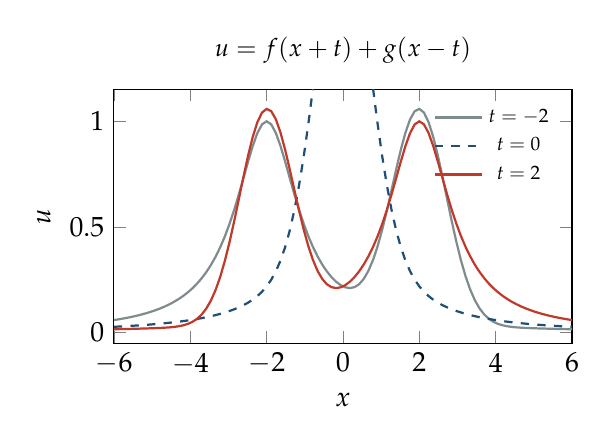
\begin{tikzpicture}
\begin{axis}[width=7.4cm,height=4.8cm,xlabel={$x$},ylabel={$u$},xmin=-6,xmax=6,ymin=-0.05,ymax=1.15,legend style={font=\scriptsize,at={(0.98,0.97)},anchor=north east,draw=none,fill=none},
 title={\small $u=f(x+t)+g(x-t)$},domain=-6:6,samples=100,no markers]
\addplot[cG,thick] {1/(1+(x+2)^2)+exp(-(x-2)^2)};
\addplot[cA,thick,dashed] {1/(1+(x+0)^2)+exp(-(x-0)^2)};
\addplot[cB,thick] {1/(1+(x-2)^2)+exp(-(x+2)^2)};
\legend{$t=-2$,$t=0$,$t=2$}
\end{axis}
\end{tikzpicture}
\hfill
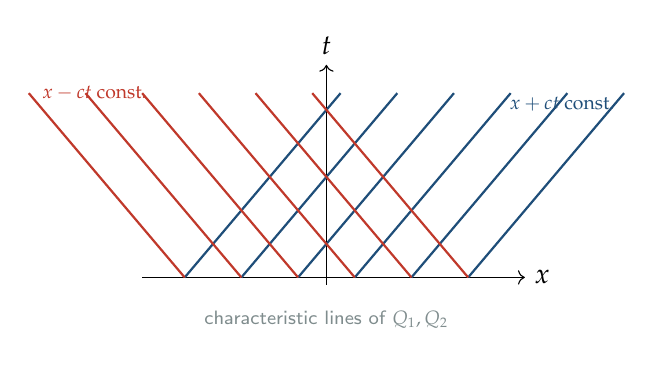
\begin{tikzpicture}[scale=0.9]
\draw[->] (-2.6,0)--(2.8,0) node[right]{$x$}; \draw[->] (0,-0.1)--(0,3) node[above]{$t$};
\foreach \a in {-2,-1.2,-0.4,0.4,1.2,2}{
  \draw[cA,thick] (\a,0)--(\a+2.2,2.6); \draw[cB,thick] (\a,0)--(\a-2.2,2.6);}
\node[cA,font=\scriptsize,anchor=west] at (2.45,2.45) {$x+ct$ const.};
\node[cB,font=\scriptsize,anchor=east] at (-2.4,2.6) {$x-ct$ const.};
\node[font=\scriptsize\sffamily,text=cG] at (0,-0.6) {characteristic lines of $Q_1,Q_2$};
\end{tikzpicture}
\caption{Left: d'Alembert solution at $t=-2,0,2$ with $c=1$; $f(x+ct)=1/(1+(x+ct)^2)$ (a lorentzian bump) moves left, $g(x-ct)=e^{-(x-ct)^2}$ (a Gaussian) moves right. Right: the two families of characteristics, one per factor $Q_1,Q_2$. Each factor of the symbol carries one rigidly translating component.}\label{fig:wave}
\end{figure}

\begin{theorem}{(Factor decomposition) \led{C12-T1$'$} \proved[]}\label{thm:factor}
Let $\Omega\subset\R^2$ be bounded, connected and simply connected, and $P=P_1^{m_1}\cdots P_N^{m_N}$ with $Q_j=P_j^{m_j}$ pairwise coprime. Then every $u\in\ker P$ (in $\mathcal D'$ or $C^\infty$) can be written
\[
u=\sum_{j=1}^Nu_j,\qquad u_j\in\ker Q_j(\partial),
\]
and the ambiguity of the decomposition is an exponential-polynomial space of dimension exactly
\[
\delta(P)=\sum_{i<j}\dimc\,\ring/(Q_i,Q_j).
\]
\end{theorem}
\begin{intuition}
This is the Chinese remainder theorem (concrete examples in Appendix~\ref{app:primer}, \S B.3; see Figure~\ref{fig:varieties}, left, for the geometric overlap). For integers coprime to each other, $\Z/ab\cong\Z/a\times\Z/b$. For polynomials in two variables, ``coprime'' does not imply $(Q_i,Q_j)=\ring$: the ideal may have a finite zero set (the points where the curves $Q_i=0$ and $Q_j=0$ cross, see Figure~\ref{fig:varieties}), and the finite quotient $\ring/(Q_i,Q_j)$ measures the overlap. Algebraically the proof uses the exact sequence
\[
0\to\ring/(Q_1Q_2)\to\ring/(Q_1)\oplus\ring/(Q_2)\to\ring/(Q_1,Q_2)\to0
\]
and the fact that $C^\infty(\Omega)$ is an injective module (a consequence of the Malgrange--Ehrenpreis theorem~\cite{eh,ma}), which turns it into an exact sequence of function spaces.
\end{intuition}

\begin{takeaway}
A ``component'' of $u$ is a \emph{factor} of the symbol, not a term of the operator. The overlap between components is finite-dimensional and exactly measured by $\delta(P)$.
\end{takeaway}

%--- E7b: Section 5.2, after the Takeaway of Theorem 5.3 ---------------------
\begin{explained}{the d'Alembert function proves Theorem~\ref{thm:factor}, step by step}
\textbf{Enunciation (Factor decomposition).} Let $\Omega\subset\R^2$ be bounded, connected and simply connected, and $P=P_1^{m_1}\cdots P_N^{m_N}$ with $Q_j=P_j^{m_j}$ pairwise coprime. Then every $u\in\ker P$ can be written $u=\sum_{j=1}^Nu_j$ with $u_j\in\ker Q_j(\partial)$, and the ambiguity of the decomposition is an exponential-polynomial space of dimension exactly $\delta(P)=\sum_{i<j}\dim\ring/(Q_i,Q_j)$.

\medskip\textbf{The case.} Wave equation, $N=2$, $m_1=m_2=1$:
\[
P=\tau^2-c^2\xi^2=Q_1Q_2,\qquad Q_1=\partial_t-c\partial_x,\quad Q_2=\partial_t+c\partial_x,
\]
and the d'Alembert solution $u=f(x+ct)+g(x-ct)$. We check each claim of the theorem.

\medskip\textbf{Step 1: the hypotheses.} $Q_1,Q_2$ are distinct linear polynomials, hence coprime (no common factor). $\Omega$ is any bounded simply connected region, e.g.\ a disc.

\medskip\textbf{Step 2: the kernels.} $Q_1f(x+ct)=cf'-cf'=0$ and $Q_2g(x-ct)=-cg'+cg'=0$, so $\ker Q_1=\{f(x+ct)\}$ (a profile moving left) and $\ker Q_2=\{g(x-ct)\}$ (a profile moving right).

\medskip\textbf{Step 3: existence of the splitting.} Take any $u\in\ker P$. Then $w_2=Q_2u\in\ker Q_1$ and $w_1=Q_1u\in\ker Q_2$ (because $Q_1Q_2u=0$). Since $Q_2-Q_1=2c\,\partial_x$,
\[
\partial_xu=\tfrac1{2c}\big(Q_2u-Q_1u\big).
\]
Integrating in $x$ at fixed $t$, define $u_1=\tfrac1{2c}\int^xQ_2u\,\dd x'$ and $u_2=-\tfrac1{2c}\int^xQ_1u\,\dd x'$. If $Q_2u=h(x+ct)$, then $u_1=\tfrac1{2c}H(x+ct)$ with $H'=h$, and $Q_1u_1=0$; likewise $u_2\in\ker Q_2$. By construction $\partial_x(u-u_1-u_2)=0$, so $u-u_1-u_2=k(t)$. Applying $P$ gives $k''(t)=0$, so $k(t)=a+bt$; and $t=\tfrac1{2c}\big((x+ct)-(x-ct)\big)$ is itself a sum of an element of $\ker Q_1$ and one of $\ker Q_2$. Hence $u=u_1+u_2$ with $u_j\in\ker Q_j$ after absorbing $k$: the splitting exists.

\medskip\textbf{Step 4: the explicit example.} With $c=1$, $u=\dfrac1{1+(x+t)^2}+e^{-(x-t)^2}$: $Q_2u=2f'(x+t)$ and $Q_1u=-2g'(x-t)$, so $u_1=\tfrac12\int^x2f'(x'+t)\dd x'=f(x+t)$ and $u_2=-\tfrac12\int^x(-2g')\dd x'=g(x-t)$, with $k=0$: the recovered components are exactly the two moving profiles.

\medskip\textbf{Step 5: the ambiguity has dimension $\delta(P)=1$.} $Q_2-Q_1=2c\,\xi$ and $Q_1+Q_2=2\tau$, so $(Q_1,Q_2)=(\tau,\xi)$, which is not the unit ideal (the two lines meet at the origin), and $\ring/(\tau,\xi)\cong\C$. So $\delta(P)=\dim\ring/(Q_1,Q_2)=1$. Directly: $f(x+ct)+g(x-ct)=0$ for all $(t,x)$ forces $f\equiv\kappa$, $g\equiv-\kappa$ for a constant $\kappa$. The only freedom is $(f,g)\mapsto(f+\kappa,g-\kappa)$: a one-dimensional space of constants, which are exponential-polynomials -- exactly the dimension the theorem predicts.

\medskip\textbf{Step 6: where the theorem's tools appear.} The finite quotient $\ring/(Q_1,Q_2)$ measures the failure of the one-variable picture. In one variable coprime polynomials satisfy a B\'ezout identity $aQ_1+bQ_2=1$ and $u=bQ_2u+aQ_1u$ splits explicitly with a direct sum; in two variables only $(Q_1,Q_2)\supseteq(\tau,\xi)$ holds, and that is what produces the constant ambiguity. The wave case is the simplest example where the proof by exact sequence $0\to\ring/(Q_1Q_2)\to\ring/(Q_1)\oplus\ring/(Q_2)\to\ring/(Q_1,Q_2)\to0$ can be followed by hand.

\medskip\textbf{Contrast with 5.1.} The same function is a sum of \emph{factor} components for every datum $(f,g)$, but a sum of \emph{term} components only when $f,g$ are polynomials. This is the difference between a factor and a term.
\end{explained}



\subsection{An explicit projector for evolution factors}
For an evolution operator with $P=\prod_{j=1}^N(\tau-a_j(\xi))$ and distinct $a_j$, a component is an eigenfunction of $\partial_t$: $\partial_tu_j=a_j(\partial_x)u_j$. Applying $\prod_{k\ne j}(\partial_t-a_k(\partial_x))$ to $u=\sum_lu_l$ kills every $u_l$ with $l\ne j$ (it contains the factor $\partial_t-a_l$) and multiplies $u_j$ by $\prod_{k\ne j}(a_j-a_k)(\partial_x)$. Hence
\begin{equation}\label{eq:lagrange}
u_j=\prod_{k\ne j}\frac{\partial_t-a_k(\partial_x)}{a_j(\partial_x)-a_k(\partial_x)}\;u ,
\end{equation}
the Lagrange formula of Eq.~\eqref{eq:spectral} with $C$ replaced by $\partial_t$. The result is a Fourier multiplier in $x$ that is rational in $\xi$, with poles where $a_j(\xi)=a_k(\xi)$; this matches the characterization ``projectors rational in $\xi$ iff the factors are coprime'' \led{II-T2/T3}.

%--- E8: Section 5.3, after Eq. (lagrange) ----------------------------------
\begin{explained}{the Lagrange projector for evolution factors}
\textbf{Step 1: the evolution operator.} $P(\tau,\xi)=\prod_{j=1}^N(\tau-a_j(\xi))$ with $a_j$ distinct polynomials in $\xi$. Replacing $\tau,\xi$ by $\partial_t,\partial_x$ the equation is $\prod_j(\partial_t-a_j(\partial_x))u=0$. Example: $a_1(\xi)=\xi$, $a_2(\xi)=-\xi$ gives $(\partial_t-\partial_x)(\partial_t+\partial_x)u=0$, the one-dimensional wave equation $u_{tt}-u_{xx}=0$. Because the factors are distinct, a solution decomposes as $u=\sum_ju_j$ where each component satisfies its own first-order law $\partial_tu_j=a_j(\partial_x)u_j$, i.e.\ $(\partial_t-a_j(\partial_x))u_j=0$.

\medskip\textbf{Step 2: isolating a component.} Fix $j$ and apply $Q_j=\prod_{k\ne j}(\partial_t-a_k(\partial_x))$ to $u=\sum_lu_l$. Constant-coefficient operators commute, so $Q_ju=\sum_lQ_ju_l$.
\begin{itemize}[nosep]
\item \emph{Case $l\ne j$.} $Q_j$ contains the factor $\partial_t-a_l(\partial_x)$, which kills $u_l$: $Q_ju_l=0$. Every component except $u_j$ disappears.
\item \emph{Case $l=j$.} No factor of $Q_j$ kills $u_j$; use $\partial_tu_j=a_j(\partial_x)u_j$: for each $k\ne j$, $(\partial_t-a_k(\partial_x))u_j=(a_j-a_k)(\partial_x)u_j$. Applying all factors, $Q_ju=\prod_{k\ne j}(a_j-a_k)(\partial_x)\,u_j$.
\end{itemize}
Hence
\[
u_j=\Big[\prod_{k\ne j}(a_j-a_k)(\partial_x)\Big]^{-1}\prod_{k\ne j}(\partial_t-a_k(\partial_x))\,u,
\]
which is Eq.~\eqref{eq:lagrange}, provided the inverse operator exists on the function space considered. It is not automatically a differential operator: it is in general a Fourier multiplier, possibly singular at frequencies where $a_j=a_k$.

\medskip\textbf{Step 3: why this is Lagrange interpolation.} The Lagrange polynomials $L_j(z)=\prod_{k\ne j}\frac{z-a_k}{a_j-a_k}$ satisfy $L_j(a_l)=1$ for $l=j$, $0$ otherwise; for a matrix $C$ diagonalized in eigenvectors, $L_j(C)$ acts as the identity on the $j$-th eigenspace and as zero on the others. Here the role of $C$ is played by $\partial_t$ and the eigenvalues $a_j$ are replaced by the operators $a_j(\partial_x)$:
\[
\Pi_j=\prod_{k\ne j}\frac{\partial_t-a_k(\partial_x)}{a_j(\partial_x)-a_k(\partial_x)},\qquad \Pi_ju=u_j .
\]
The analogy is exact at the algebraic level: $\Pi_j$ is the projector that extracts the $j$-th evolution component.

\medskip\textbf{Step 4: rational in $\xi$.} With the Fourier convention $\partial_x\mapsto i\kappa$ ($\kappa$ real frequency), $a_j(\partial_x)$ becomes multiplication by $a_j(i\kappa)$ and the multiplier is
\[
\ell_j(\kappa,\partial_t)=\prod_{k\ne j}\frac{\partial_t-a_k(i\kappa)}{a_j(i\kappa)-a_k(i\kappa)} .
\]
The denominators vanish exactly where $a_j(i\kappa)=a_k(i\kappa)$: these are the potential poles of the projector. Strictly, the rationality concerns the dependence on the spatial frequency; the projector still involves $\partial_t$ before it is restricted to a solution component, on which $\partial_t$ acts as multiplication by $a_j(i\kappa)$.

\medskip\textbf{Step 5: the wave equation.} $(\partial_t-\partial_x)(\partial_t+\partial_x)u=0$, $u=u_1+u_2$ with $\partial_tu_1=\partial_xu_1$ and $\partial_tu_2=-\partial_xu_2$. Applying $\partial_t+\partial_x$: the $u_2$ term vanishes and $(\partial_t+\partial_x)u_1=2\partial_xu_1$, so
\[
u_1=\tfrac12\,\partial_x^{-1}(\partial_t+\partial_x)u,\qquad u_2=-\tfrac12\,\partial_x^{-1}(\partial_t-\partial_x)u .
\]
In Fourier variables $\partial_x^{-1}$ is multiplication by $1/(i\kappa)$: a pole at $\kappa=0$. This does not mean the wave equation has no decomposition (Section~\ref{sec:fact} proves it does), only that this particular formula needs a choice of inverse (an integration constant) or extra assumptions at zero frequency.

\medskip\textbf{Step 6: what ``coprime'' means.} $\tau-a_j(\xi)$ and $\tau-a_k(\xi)$ are coprime in $\C[\tau,\xi]$ exactly when $a_j-a_k$ is not the zero polynomial; for distinct $a_j$ this holds, though $a_j-a_k$ may still vanish at particular frequencies, creating poles. Three levels must be kept apart: \emph{coprime factors} (the algebraic decomposition exists in the localized, rational-operator sense); \emph{no poles at any frequency} (stronger, not guaranteed by coprimality); \emph{a bounded or well-defined projector on a chosen function space} (needs analytic conditions near frequencies where branches meet). The message: distinct evolution branches admit algebraic projectors, like distinct eigenvalues of a matrix; in spatial Fourier variables the projectors are rational multipliers whose denominators reveal where the branches intersect.
\end{explained}



\subsection{Where decomposition fails}
\begin{proposition}{(Holes) \led{C12-P10} \proved[]}
On a domain with a hole, the decomposition fails for some $P$.
\end{proposition}
Figure~\ref{fig:hole} shows the standard obstruction. In the theorem the hypothesis ``simply connected'' means $H^1_{dR}(\Omega)=0$, exactly what removes this obstruction; a cohomological criterion for non-simply connected $\Omega$ is also available \led{OP-FUN, C12-Q6}.
\begin{figure}[!htb]
\centering
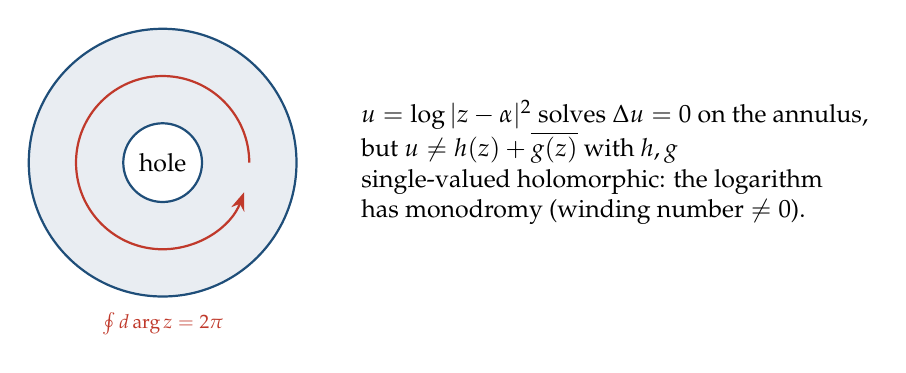
\begin{tikzpicture}
\fill[cA!10] (0,0) circle (1.7); \fill[white] (0,0) circle (0.5);
\draw[cA,thick] (0,0) circle (1.7); \draw[cA,thick] (0,0) circle (0.5);
\node at (0,0) {\small hole};
\draw[cB,thick,-{Stealth}] (1.1,0) arc (0:340:1.1);
\node[cB,font=\scriptsize] at (0,-2.05) {$\oint d\arg z=2\pi$};
\node[align=left,font=\small,anchor=west] at (2.4,0) {$u=\log|z-\alpha|^2$ solves $\Delta u=0$ on the annulus,\\ but $u\neq h(z)+\overline{g(z)}$ with $h,g$\\ single-valued holomorphic: the logarithm\\ has monodromy (winding number $\neq0$).};
\end{tikzpicture}
\caption{The Laplacian $\partial_x^2+\partial_y^2=(\partial_x+i\partial_y)(\partial_x-i\partial_y)$ factors, but the factor decomposition fails on a punctured disc: the obstruction is topological ($H^1_{dR}\neq0$).}\label{fig:hole}
\end{figure}

\subsection{Regularity: when are the components in $H^m$?}
The decomposition is an algebraic statement; analysis enters when we want components in a Sobolev space. For two components the governing condition is geometric: the two component spaces $M_1$ and $M_2$ must be separated by a positive angle (Figure~\ref{fig:friedrichs}); the next theorem makes this precise for any number of components. Two difficulties appear along the way; they are collected in the box after the theorem.
\begin{proposition}{(Loss of a derivative) \led{C12-C1} \falsest}\label{prop:loss}
``If $u\in H^m(\Omega)$ then all $u_j\in H^m$'' is false: one derivative can be lost. In other words, the pieces of a smooth function may be rougher than the function itself.
\end{proposition}
\begin{theorem}{(Regularity criterion) \led{C12-T3, C12-P7} \proved[]}\label{thm:hm}
All components lie in $H^m$ for every $u\in\ker_{H^m}P$ iff the sum $\sum_j\ker_{H^m}Q_j$ is \emph{closed} and \emph{dense} in $\ker_{H^m}P$. Closedness is equivalent to $\gamma_N>0$, where
\[
\begin{aligned}
\gamma_N&=\inf\sigma\big(S^*S\big|_{(\ker S)^\perp}\big),\\
S&:\bigoplus_{j=1}^N\ker Q_j\to H^m,\qquad S(u_1,\dots,u_N)=\sum_{j=1}^Nu_j .
\end{aligned}
\]
For $N=2$ this is the condition $c_F<1$ on the Friedrichs cosine. Density holds on every bounded convex $\Omega$, for every $P$ and $m$ \led{OPF5B-T1} \modulo{H\"ormander~\cite{ho}, Stein}.
\end{theorem}
\begin{notebox}{Reading $\gamma_N$}
\begin{itemize}[nosep]
\item The space $\bigoplus_j\ker Q_j$ consists of the $N$-tuples $v=(u_1,\dots,u_N)$ with norm $\|v\|^2=\sum_j\|u_j\|_{H^m}^2$;
\item $Sv=\sum_ju_j$ is their sum;
\item $S^*$ is the adjoint of $S$;
\item $(\ker S)^\perp$ removes the tuples that sum to zero (the ambiguity of Theorem~\ref{thm:factor});
\item $\inf\sigma$ is the bottom of the spectrum.
\end{itemize}
Since $S^*S$ restricted to $(\ker S)^\perp$ is self-adjoint and nonnegative, the bottom of its spectrum is the minimum of the Rayleigh quotient
\[
\frac{\langle S^*Sv,v\rangle}{\|v\|^2}=\frac{\|Sv\|^2}{\|v\|^2}.
\]
Hence the formula of the theorem is equivalent to the more intuitive
\[
\boxed{\ \gamma_N=\inf_{\substack{v\in(\ker S)^\perp\\ v\ne0}}\frac{\|Sv\|_{H^m}^2}{\|v\|^2}\ }
\]
\end{notebox}

\begin{aside}{In words}
$\gamma_N$ is the worst case, over all tuples of pieces, of the ratio between the size of the sum and the size of the pieces.
\begin{itemize}[nosep]
\item If $\gamma_N>0$ the pieces cannot nearly cancel each other, and
\[
\|v\|\le\gamma_N^{-1/2}\|Sv\|:
\]
the pieces are controlled by the sum, so recovering them from $u$ is stable.
\item If $\gamma_N\to0$ there are large pieces whose sum is tiny, and the recovery is unstable.
\end{itemize}
\textbf{The case $N=2$.} One finds $\gamma_2=1-c_F$, where
\[
c_F=\sup\{|\langle a,b\rangle|:\ a\in M_1\ominus(M_1\cap M_2),\ b\in M_2\ominus(M_1\cap M_2),\ \|a\|=\|b\|=1\}
\]
is the Friedrichs cosine: the part of $v$ lying in $M_1\cap M_2$ contributes the ratio $2$ and does not affect the infimum, and on the rest
\[
\|a+b\|^2\ge(1-c_F)(\|a\|^2+\|b\|^2)
\]
with near-equality attained. Hence $c_F<1\iff\gamma_2>0$, as stated.
\end{aside}
\begin{figure}[!htb]
\centering
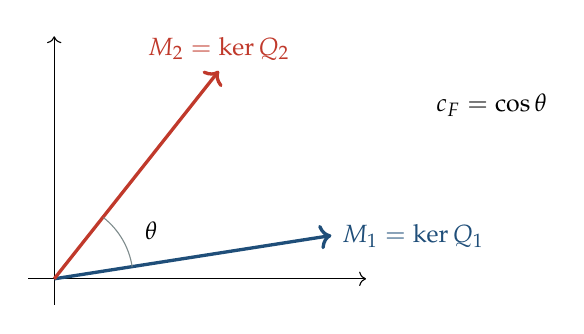
\begin{tikzpicture}[scale=1.1]
\draw[->] (-0.3,0)--(3.6,0); \draw[->] (0,-0.3)--(0,2.8);
\draw[cA,very thick,->] (0,0)--(3.2,0.5) node[right,font=\small]{$M_1=\ker Q_1$};
\draw[cB,very thick,->] (0,0)--(1.9,2.4) node[above,font=\small]{$M_2=\ker Q_2$};
\draw[cG] (0.9,0.14) arc (8.9:51.6:0.9); \node[font=\small] at (1.12,0.55) {$\theta$};
\node[font=\small,anchor=west] at (4.3,2.0) {$c_F=\cos\theta$};



\end{tikzpicture}
\caption{Friedrichs angle $\theta$ between two component spaces $M_1=\ker Q_1$ and $M_2=\ker Q_2$. A larger angle means a better-conditioned recovery of the pieces from their sum.}\label{fig:friedrichs}
\end{figure}
For $N=2$, Figure~\ref{fig:friedrichs} reads as follows: $c_F=\cos\theta$; if $\theta>0$ the sum $M_1+M_2$ is closed and the pieces depend continuously on $u$; as $\theta\to0$ the split becomes unstable. For $N\ge3$ the pairwise angles do not suffice; $\gamma_N$, the smallest nonzero eigenvalue of $S^*S$, is the right conditioning number: it is the conditioning of the linear map ``components $\mapsto$ sum'', exactly like the smallest nonzero singular value in a least-squares problem.

\begin{caution}[title=Two problems with regularity]
\textbf{Problem 1: stability \falsest.} Algebraically the split always exists (Theorem~\ref{thm:factor}), but the pieces may be less regular than $u$. When the angle between the component spaces tends to $0$ (that is, $\gamma_N\to0$) the map ``$u\mapsto$ pieces'' becomes unstable, and one derivative can be lost (Proposition~\ref{prop:loss}). For the algorithm: check $\gamma_N>0$ before using the components in $H^m$ (Step~5).\\[3pt]
\textbf{Problem 2: three or more components \openq.} For $N\ge3$ the pairwise cosines $c_F(i,j)$ do not decide whether the sum of kernels is closed: an abstract Hilbert-space counterexample exists \led{S-CHECK-4}, and whether it can occur for differential operators is open \led{C12-Q2}.
\end{caution}

%--- E9: Section 5.5, just before the final Takeaway of Section 5 -----------
\begin{explained}{regularity, the sum map $S$, $\gamma_N$ and the Friedrichs angle}
\textbf{The guiding idea.} $\gamma_N$ measures \emph{how reliably a solution can be separated into components belonging to different kernel spaces, and how much errors can be amplified when this is done}. Being able to decompose algebraically does not guarantee that the pieces have the regularity of the original solution; the obstruction is geometric: the component spaces may be too close to one another, which makes the decomposition unstable.

\medskip\textbf{Step 1: why a component can lose a derivative.} $Pu=0$, $u=\sum_ju_j$, $Q_ju_j=0$. The pieces exist, but $u\in H^m$ does not imply $u_j\in H^m$, because the formulas that extract $u_j$ may involve inverse differential operators, which can lose regularity. In the wave example $u_1=\tfrac12\partial_x^{-1}(\partial_t+\partial_x)u$: even if $u$ has $m$ Sobolev derivatives the formula alone does not guarantee that $u_1$ has $m$, because of the inverse and its behaviour at problematic frequencies. This is the content of Proposition~\ref{prop:loss}.

\medskip\textbf{Step 2: the component spaces and the sum operator.} $M_j=\ker_{H^m}Q_j$ (admissible components); for two components $M=\ker_{H^m}Q_1$, $N=\ker_{H^m}Q_2$. The decomposition question is packaged in
\[
S:M_1\times\cdots\times M_N\to H^m(\Omega),\qquad S(u_1,\dots,u_N)=\sum_ju_j,\qquad \|(u_1,\dots,u_N)\|^2=\sum_j\|u_j\|_{H^m}^2 .
\]
Recovering the components means inverting $S$ on the relevant solution space. Two things can go wrong: \emph{non-uniqueness} (different tuples with the same sum: $\ker S=\{(u_j):\sum u_j=0\}$; if $v\in M\cap N$ then $(v,-v)\in\ker S$, so overlapping spaces give non-uniqueness) and \emph{instability} (even if unique, a tiny change in the sum may require a large change in the pieces).

\medskip\textbf{Step 3: what $\gamma_N$ is.}
\[
\gamma_N=\inf\sigma\big(S^*S|_{(\ker S)^\perp}\big)=\inf_{\substack{v\in(\ker S)^\perp\\v\ne0}}\frac{\|Sv\|_{H^m}^2}{\|v\|^2}.
\]
$S^*$ is the adjoint, $S^*S$ is positive self-adjoint, and $(\ker S)^\perp$ removes the directions that change the pieces without changing the sum (without this removal the ratio would be $0$ regardless of the stability of the genuinely recoverable part). If $\gamma_N>0$ then $\|Sv\|^2\ge\gamma_N\|v\|^2$ on $(\ker S)^\perp$, i.e.
\[
\|v\|\le\gamma_N^{-1/2}\|Sv\|:
\]
this is the stability estimate; the smaller $\gamma_N$, the larger the possible amplification. \emph{Technical caveat:} if the restriction has continuous spectrum accumulating at $0$, ``smallest nonzero eigenvalue'' (used loosely in the text after Figure~\ref{fig:friedrichs}) is not literally correct; the robust quantity is the \emph{infimum of the spectrum} on $(\ker S)^\perp$, as in the theorem.

\medskip\textbf{Step 4: two components and the Friedrichs angle.} Let $I=M\cap N$. The Friedrichs cosine is $c_F=\sup\{|\langle x,y\rangle|:x\in M\cap I^\perp,\ y\in N\cap I^\perp,\ \|x\|=\|y\|=1\}$, and $\theta\in[0,\pi/2]$ is defined by $c_F=\cos\theta$. If $c_F$ is close to $1$ the spaces have almost parallel directions; if it is clearly below $1$ they are well separated; $c_F<1$ means the sum $M+N$ is closed. A finite-dimensional analogy: decomposing a vector along two nearly parallel directions gives large components that nearly cancel, leaving a small sum; recovering them from the small sum is numerically unstable. The paper proves $\gamma_2=1-c_F$, so $c_F<1\iff\gamma_2>0$.

\medskip\textbf{Step 5: why pairwise angles do not suffice for $N\ge3$.} Three vectors in a plane pointing in three different directions can satisfy $v_1+v_2+v_3=0$: the instability depends on combinations of all components, not only on pairs. $S$ captures these collective effects; its smallest nonzero singular value is $\sqrt{\gamma_N}$, so $1/\sqrt{\gamma_N}$ is the natural condition-number-like factor for recovering components from their sum, as in a least-squares problem where a small singular value makes inversion sensitive to errors.

\medskip\textbf{Step 6: density.} The theorem needs $M_1+\dots+M_N$ to be both closed and dense in $\ker_{H^m}P$. Dense plus closed gives $M_1+\dots+M_N=\ker_{H^m}P$, i.e.\ a decomposition for every solution, with stability from the positive-angle condition. The text states density on bounded convex domains for every $P$ and $m$ (H\"ormander, Stein; see its status label), so closedness is the decisive remaining condition there.

\medskip\textbf{The chain in six lines.} (1) Algebra produces components attached to the factors. (2) Sobolev asks whether they remain in $H^m$. (3) This is controlled by $S$. (4) $\gamma_N>0$ makes $S$ bounded below after removing its kernel: stable recovery. (5) For $N=2$ this is $c_F<1$. (6) For $N\ge3$ the collective $\gamma_N$, not the pairwise angles, controls the conditioning. One distinction: $\gamma_N>0$ is about the stability of the decomposition map; it is not an algebraic statement about factorization. The factorization says which spaces to consider, their geometry in $H^m$ says whether the components can be recovered with the desired regularity.
\end{explained}


\begin{takeaway}
Algebraically the split always exists (Theorem~\ref{thm:factor}); analytically, the components are well behaved exactly when the component spaces are separated by a positive angle (Theorem~\ref{thm:hm}). The next section stops asking for a split into factors and asks what survives when one splits by additive terms instead.
\end{takeaway}

%======================================================================
\section{Terms inside a factor and the interaction term}\label{sec:terms}
\sectionbrief
{an evolution equation $u_t=Au$, $A=A_1+\dots+A_N$ (the terms), with flows $S_n(t)=e^{tA_n}$; the terms commute, except in the last subsection of this section (non-commuting terms).}
{Proposition~\ref{prop:terms} shows that splitting by terms is never exact; here we compute exactly what is left over (the interaction term $\Eint$), its cost, and its stability.}
{third link of the chain, answering Q3. \emph{Result:} an exact product formula, a cost dichotomy $O(N)$ versus $\Theta(2^N)$, and a negative stability theorem.}

Here the equation is an evolution $u_t=Au$ with $A=A_1+\dots+A_N$, each $A_n$ a \emph{term} (diffusion, advection, reaction, \dots).

\begin{aside}{From summing operators to the interaction term}
The solution is
\[
u(t)=e^{tA}u_0=S(t)u_0,
\]
where $S(t)=e^{tA}$ is the \emph{flow} (semigroup) generated by $A$. If term $n$ acted alone, it would produce $S_n(t)u_0=e^{tA_n}u_0$, a change of $S_n(t)u_0-u_0$.

The naive guess is that the terms act independently, so that the total change $u(t)-u_0$ is the sum of the individual changes. It is not: the flow of a sum is not the sum of the flows. For advection ($A_1=-c\partial_x$, a translation) and diffusion ($A_2=D\partial_x^2$, a smoothing) the solution is translated \emph{and} smoothed, and this joint action is not ``only translated'' plus ``only smoothed''. What is missing is the \emph{interaction term} $\Eint$ defined next.

The section proceeds in three steps:
\begin{enumerate}[nosep]
\item define $\Eint$ (6.1);
\item compute it exactly when the terms commute, using Fourier variables (6.2);
\item measure its cost (6.3) and its stability (6.4).
\end{enumerate}
Subsections 6.5 and 6.6 treat the cases without a closed formula.
\end{aside}

\subsection{Definition via the flows of the single terms}
Let $S(t)=e^{tA}$ and $S_n(t)=e^{tA_n}$. The contribution that term $n$ \emph{alone} would make to the solution is $S_n(t)u_0-u_0$. The remainder is the interaction term
\begin{equation}\label{eq:eint-def}
\Eint^{\mathrm{add}}(t)=u(t)-u_0-\sum_{n=1}^N\big(S_n(t)u_0-u_0\big).
\end{equation}
(The superscript ``add'' records that this is the \emph{additive} definition; below we write $\Eint$ for $\Eint^{\mathrm{add}}$ unless the distinction matters.)

\subsection{Exact formula in the commuting case}
\begin{aside}{Why constant coefficients commute, and what $\Delta_n$ is}
Constant-coefficient operators are polynomials in $\partial_t,\partial_x$ (Section~\ref{sec:prelim}) and the ring $\ring$ is commutative, so any two terms commute: $A_1A_2=A_2A_1$. For commuting operators
\[
e^{t(A_1+A_2)}=e^{tA_1}e^{tA_2},\qquad\text{hence}\qquad S=\prod_nS_n;
\]
without commutativity this fails (Section~\ref{sec:noncomm}).

We call
\[
\Delta_n=S_n(t)-\Id
\]
the \emph{increment} produced by term $n$ alone, where $\Id$ is the identity operator and $t$ is fixed; thus $S_n=\Id+\Delta_n$, and $\Delta_nu_0=S_n(t)u_0-u_0$ is exactly the contribution of term $n$ in \eqref{eq:eint-def}. Products of operators are compositions.
\end{aside}

\begin{notebox}{Fourier variables}
For constant coefficients it is convenient to pass to Fourier variables. With
\[
\hat u(\kappa)=\int u(x)e^{-i\kappa x}\dd x,
\]
where $\kappa\in\R$ is the frequency:
\begin{itemize}[nosep]
\item the derivative $\partial_x$ becomes multiplication by $i\kappa$;
\item each term $A_n$ becomes multiplication by its \emph{symbol} $a_n(\kappa)$ (a polynomial in $i\kappa$);
\item $e^{tA_n}$ becomes multiplication by the number $e^{ta_n(\kappa)}$.
\end{itemize}
Operators turn into numbers and compositions into products of numbers, so for a fixed $\kappa$ every computation below is scalar.
\end{notebox}
\begin{theorem}{(Interaction term) \led{P1-T2, P1-T3} \proved[]}\label{thm:eint}
Assume the $A_n$ commute (e.g.\ constant coefficients). Write $\Delta_n=S_n(t)-\Id$. Then
\begin{equation}\label{eq:eint}
\Eint^{\mathrm{add}}=\Big[\prod_{n=1}^N(\Id+\Delta_n)-\Id-\sum_{n=1}^N\Delta_n\Big]u_0 .
\end{equation}
For $N=2$ this is simply $\Eint=\Delta_1\Delta_2u_0=(S_1-\Id)(S_2-\Id)u_0$. In Fourier variables, with $\hat A_n=a_n(\kappa)$,
\[
\widehat{\Eint}(t,\kappa)=\Big[\prod_n\big(e^{ta_n(\kappa)}\big)-1-\sum_n\big(e^{ta_n(\kappa)}-1\big)\Big]\hat u_0(\kappa).
\]
\end{theorem}
\begin{proof}
Commutation gives $S=e^{t\sum A_n}=\prod_nS_n$. Substitute $S_n=\Id+\Delta_n$ in \eqref{eq:eint-def}. For $N=2$, expand the product:
\[
\begin{aligned}
S_1S_2&=(\Id+\Delta_1)(\Id+\Delta_2)\\
&=\Id+\Delta_1+\Delta_2+\Delta_1\Delta_2 ,
\end{aligned}
\]
and $\sum_n(S_n-\Id)=\Delta_1+\Delta_2$, so the remainder in \eqref{eq:eint-def} is $\Delta_1\Delta_2u_0$.

For general $N$, the $\Delta_n$ commute, so
\[
\prod_n(\Id+\Delta_n)=\sum_{S\subseteq\{1,\dots,N\}}\prod_{n\in S}\Delta_n ;
\]
removing the subsets with $|S|=0$ and $|S|=1$ leaves
\[
\Eint=\sum_{|S|\ge2}\Delta_S\,u_0,\qquad \Delta_S=\prod_{n\in S}\Delta_n .
\]
In words: the interaction is the sum of products of at least two increments, and appears only when at least two terms act together.
\end{proof}

%--- E11: Section 6.2, after the proof of Theorem 6.1 (before the concrete case)
\begin{explained}{the additive interaction remainder and why the terms commute}
\textbf{Step 1: the setup.} $\partial_tu=Au$, $u(0)=u_0$, with $A=\sum_{n=1}^NA_n$. The solution is formally $u(t)=e^{tA}u_0$. If term $n$ acted alone it would produce $S_n(t)=e^{tA_n}$, with change $\Delta_nu_0=(S_n(t)-\Id)u_0$ ($\Delta_n$ is the \emph{increment operator}). The additive interaction remainder is
\[
\Eint^{\mathrm{add}}(t)=u(t)-u_0-\sum_{n=1}^N\Delta_nu_0,
\]
that is, \emph{interaction $=$ full evolution $-$ initial state $-$ sum of the individual increments.}
Note that this is an additive decomposition, \emph{not} a decomposition into kernel spaces as in Section~\ref{sec:fact}.

\medskip\textbf{Step 2: why commutation gives an exact formula.} If $A_iA_j=A_jA_i$ then (for suitable operators and a well-defined evolution) $e^{t\sum_nA_n}=\prod_ne^{tA_n}=\prod_nS_n(t)$. Since $S_n=\Id+\Delta_n$,
\[
u(t)=\prod_{n=1}^N(\Id+\Delta_n)u_0,\qquad
\Eint^{\mathrm{add}}(t)=\Big[\prod_{n=1}^N(\Id+\Delta_n)-\Id-\sum_{n=1}^N\Delta_n\Big]u_0 .
\]
This is pure algebra: multiply the increments, then subtract the constant term and all terms involving a single increment.

\medskip\textbf{Step 3: $N=2$.} $u(t)=S_1S_2u_0=(\Id+\Delta_1)(\Id+\Delta_2)u_0=(\Id+\Delta_1+\Delta_2+\Delta_1\Delta_2)u_0$. Subtracting $u_0$ and the two single increments leaves
\[
\Eint^{\mathrm{add}}(t)=\Delta_1\Delta_2u_0=(S_1-\Id)(S_2-\Id)u_0 .
\]
It is an interaction term because it contains the effect of both increments acting together; if either increment is zero on the relevant state, the interaction vanishes.

\medskip\textbf{Step 4: $N=3$ shows the general structure.}
\[
(\Id+\Delta_1)(\Id+\Delta_2)(\Id+\Delta_3)=\Id+\Delta_1+\Delta_2+\Delta_3+\Delta_1\Delta_2+\Delta_1\Delta_3+\Delta_2\Delta_3+\Delta_1\Delta_2\Delta_3,
\]
so $\Eint^{\mathrm{add}}=(\Delta_1\Delta_2+\Delta_1\Delta_3+\Delta_2\Delta_3+\Delta_1\Delta_2\Delta_3)u_0$: three \emph{pairwise} interactions and one \emph{three-way} interaction. In general $\Eint^{\mathrm{add}}=\sum_{J\subseteq\{1,\dots,N\},|J|\ge2}\big(\prod_{j\in J}\Delta_j\big)u_0$: the empty subset gives the initial state, subsets of size one the individual increments, everything left involves at least two operators.

\medskip\textbf{Step 5: the Fourier formula.} If each $A_n$ is a constant-coefficient operator it becomes multiplication by its symbol $a_n(\kappa)$, so $\widehat{S_n(t)u_0}=e^{ta_n(\kappa)}\hat u_0$ and $\widehat{\Delta_nu_0}=(e^{ta_n(\kappa)}-1)\hat u_0$. Then
\[
\widehat{\Eint^{\mathrm{add}}}(t,\kappa)=\Big[\prod_ne^{ta_n(\kappa)}-1-\sum_n\big(e^{ta_n(\kappa)}-1\big)\Big]\hat u_0(\kappa).
\]
At each frequency this is ordinary scalar algebra; the operators commute because their Fourier symbols are multiplications. \emph{Notation note:} here $\kappa$ is the real frequency and $a_n(\kappa)$ the symbol of $A_n$ in the variable $i\kappa$ (e.g.\ $a(\kappa)=-ic\kappa-D\kappa^2$ for advection--diffusion).

\medskip\textbf{Step 6: small-time reading.} $\Delta_n=e^{tA_n}-\Id=tA_n+O(t^2)$. For two operators, $\Eint^{\mathrm{add}}=\Delta_1\Delta_2u_0=t^2A_1A_2u_0+O(t^3)$ (given enough regularity). Each single increment starts at order $t$, their interaction at order $t^2$: it needs both effects to contribute. For $N$ operators the interaction involving all $N$ increments starts at $t^N$, while the full remainder also contains pairwise interactions, generally starting at $t^2$.

\medskip\textbf{Step 7: why the terms commute.} Two operators that are polynomials in the \emph{same} $\partial_x$, e.g.\ $A_1=a_0+a_1\partial_x+a_2\partial_x^2$ and $A_2=b_0+b_1\partial_x+b_2\partial_x^2$, commute because powers of $\partial_x$ commute: $[A_1,A_2]=0$. More generally any two constant-coefficient operators, polynomials in $\partial_{x_1},\dots,\partial_{x_d}$, commute; for instance $A_1=\partial_x^2+\partial_y$ and $A_2=3\partial_x\partial_y-\partial_y^2$, because partial derivatives commute on sufficiently smooth functions (and on distributions). So for constant coefficients commutation is not a restrictive hypothesis: it comes almost automatically from the structure of the operators.

\medskip\textbf{The conceptual contrast.} Section~\ref{sec:fact} asked whether a solution can be stably separated into pieces belonging to different kernels. Here the question is different: if the generator is a sum of operators, how much of the resulting evolution cannot be explained by adding their individual changes? When the operators commute the answer is exact: expand the product of the evolution operators, remove the initial state and the single-operator contributions, and what remains is exactly the mixed interaction terms.
\end{explained}



\paragraph{A concrete case.}\label{par:advdiff}
Take advection--diffusion, $u_t=-cu_x+Du_{xx}$, with Gaussian datum $u_0=g(x;\sigma^2)$, where $g(x;v)=e^{-x^2/2v}/\sqrt{2\pi v}$. The two flows act as a translation and a Gaussian smoothing:
\[
S_1u_0=g(x-ct;\sigma^2),\qquad S_2u_0=g(x;s^2),\qquad u=g(x-ct;s^2),\qquad s^2=\sigma^2+2Dt .
\]
Hence
\[
\Eint=g(x-ct;s^2)-g(x-ct;\sigma^2)-g(x;s^2)+g(x;\sigma^2).
\]
Figure~\ref{fig:eint}(a) plots it: it is comparable in size to $u$ itself, so it cannot be discarded as a small correction. In Fourier variables the ratio $|\widehat{\Eint}|/|\hat u_0|=|(e^{-ic\kappa t}-1)(e^{-D\kappa^2t}-1)|$ is at most $2$; it vanishes at $\kappa=0$ and whenever $c\kappa t\in2\pi\mathbb Z$ (the translation returns to the identity), see Figure~\ref{fig:eint}(b).

\begin{figure}[!htb]
\centering
\begin{tikzpicture}
\begin{axis}[width=7.6cm,height=5.6cm,xlabel={$x$},xmin=-6,xmax=8,ymin=-0.2,ymax=0.45,
 title={\small (a) $u_t=-cu_x+Du_{xx}$, $t=1$, $c=2$, $D=\tfrac12$},legend style={font=\scriptsize,draw=none,fill=white,fill opacity=0.8,text opacity=1,at={(0.02,0.98)},anchor=north west},
 domain=-6:8,samples=140,no markers]
\addplot[cG,thick,dashed] {gauss(x,1)};
\addplot[cA,thick] {gauss(x-2,2)};
\addplot[cB,very thick] {gauss(x-2,2)-gauss(x-2,1)-gauss(x,2)+gauss(x,1)};
\legend{$u_0$,$u(t)$,$\Eint$}
\end{axis}
\end{tikzpicture}\hfill
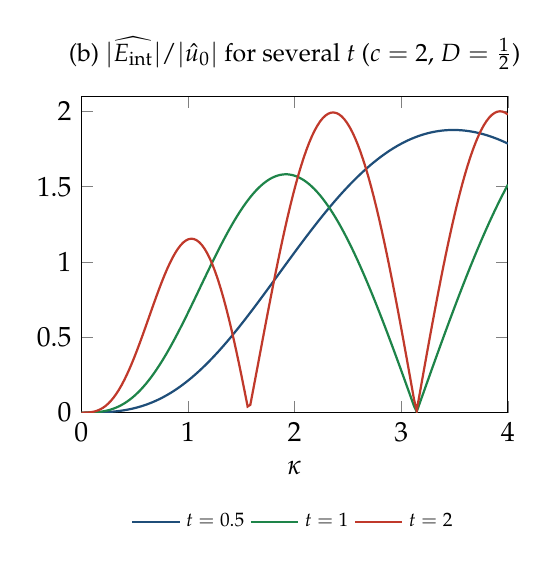
\begin{tikzpicture}
\begin{axis}[width=7.0cm,height=5.6cm,xlabel={$\kappa$},xmin=0,xmax=4,ymin=0,ymax=2.1,
 title={\small (b) $|\widehat{\Eint}|/|\hat u_0|$ for several $t$ ($c=2$, $D=\tfrac12$)},legend style={font=\scriptsize,draw=none,at={(0.5,-0.28)},anchor=north,legend columns=3},
 domain=0:4,samples=160,no markers]
\addplot[cA,thick] {sqrt(((cos(deg(2*0.5*x))-1)^2+sin(deg(2*0.5*x))^2)*(exp(-0.5*0.5*x^2)-1)^2)};
\addplot[cC,thick] {sqrt(((cos(deg(2*1.0*x))-1)^2+sin(deg(2*1.0*x))^2)*(exp(-0.5*1.0*x^2)-1)^2)};
\addplot[cB,thick] {sqrt(((cos(deg(2*2.0*x))-1)^2+sin(deg(2*2.0*x))^2)*(exp(-0.5*2.0*x^2)-1)^2)};
\legend{$t=0.5$,$t=1$,$t=2$}
\end{axis}
\end{tikzpicture}
\caption{Advection--diffusion with Gaussian datum ($\sigma^2=1$, $c=2$, $D=\tfrac12$). (a) $u_0$, $u(t)$ and $\Eint$ at $t=1$. (b) The Fourier ratio $|\widehat{\Eint}|/|\hat u_0|$ for three times.}\label{fig:eint}
\end{figure}

\subsection{Cost: $O(N)$ versus $2^N$}
Expanding \eqref{eq:eint} in the $\Delta_n$ produces one monomial per subset of $\{1,\dots,N\}$ with at least two elements: $2^N-N-1$ cross terms (Figure~\ref{fig:lattice}: the red nodes are the cross terms). Writing the \emph{complete table} of cross terms is therefore exponential. Evaluating a \emph{value} is cheap, because we never expand the product. The algorithm uses exactly the product (Fourier) form of Theorem~\ref{thm:eint},
\[
\widehat{\Eint}(t,\kappa)=\Big[\prod_{n=1}^Ne^{ta_n(\kappa)}-1-\sum_{n=1}^N\big(e^{ta_n(\kappa)}-1\big)\Big]\hat u_0(\kappa),
\]
which for a fixed $\kappa$ needs the $N$ numbers $e^{ta_n(\kappa)}$, $N-1$ products and $N$ subtractions: $O(N)$ operations once $\hat u_0(\kappa)$ is known.
\begin{aside}{Two remarks on cost}
\textbf{What ``value'' means.} Here ``value'' means one Fourier value; recovering $\Eint(t,x)$ at a point of space needs an inverse Fourier transform, whose cost is not counted in the $O(N)$.

\textbf{Where $2^N$ comes from.} The count $2^N-N-1$ refers only to writing out all cross terms one by one; the product form never does so (Step~6 of the algorithm).
\end{aside}
\begin{figure}[!htb]
\centering
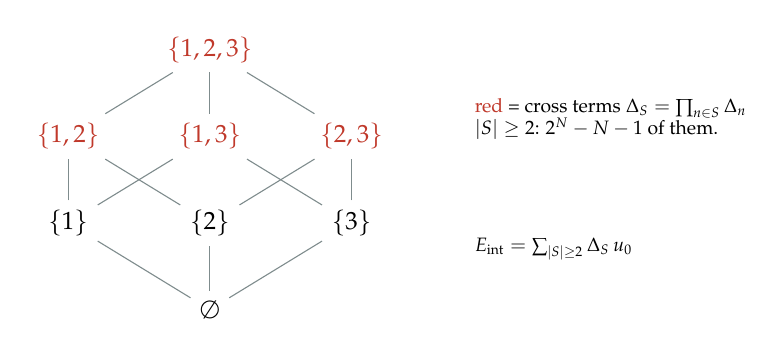
\begin{tikzpicture}[x=1.8cm,y=1.1cm,every node/.style={font=\small}]
\node (e) at (0,0) {$\emptyset$};
\node (1) at (-1,1) {$\{1\}$}; \node (2) at (0,1) {$\{2\}$}; \node (3) at (1,1) {$\{3\}$};
\node[text=cB] (12) at (-1,2) {$\{1,2\}$}; \node[text=cB] (13) at (0,2) {$\{1,3\}$}; \node[text=cB] (23) at (1,2) {$\{2,3\}$};
\node[text=cB] (123) at (0,3) {$\{1,2,3\}$};
\foreach \a/\b in {e/1,e/2,e/3,1/12,1/13,2/12,2/23,3/13,3/23,12/123,13/123,23/123} \draw[cG] (\a)--(\b);
\node[anchor=west,align=left,font=\scriptsize] at (1.8,2.2) {\textcolor{cB}{red} = cross terms $\Delta_S=\prod_{n\in S}\Delta_n$\\ $|S|\ge2$: $2^N-N-1$ of them.};
\node[anchor=west,align=left,font=\scriptsize] at (1.8,0.7) {$\Eint=\sum_{|S|\ge2}\Delta_S\,u_0$};
\end{tikzpicture}
\caption{Subset lattice for $N=3$ terms: one node per subset $S$ of terms, one monomial $\Delta_S$ per node with $|S|\ge2$. The count $2^N-N-1$ is what makes the full table exponential.}\label{fig:lattice}
\end{figure}
\begin{proposition}{(Complexity) \led{P1-T3} \proved[]}
In the commuting exponential-type class, a value of $\Eint$ costs $O(M(N+\sum d))$ for $M$ evaluation points; aggregated by order $O(MN^2)$; the full table $\Theta(M2^N(L+1)^2)$.
\end{proposition}
\edmark{E1}

\subsection{Why $\Eint$ cannot be removed or regularized stably}
The cost question being settled, we ask whether $\Eint$ can be suppressed by a regularization, or at least depends continuously on the datum.
\begin{proposition}{(Not continuous in $H^m$) \led{P1-P1(e)} \falsest}\label{prop:discont}
The map $u_0\mapsto\Eint(t)$ is \emph{not} continuous in $H^m(\Omega)$ for advection--diffusion, for any $m$ and any $t$; the same holds for any two non-proportional terms \led{P1-Q6}.
\end{proposition}
Consequently:
\begin{itemize}[nosep]
\item \textbf{A sparsity (or $L^2$) penalty cannot make $\Eint$ vanish.} Outside a finite-dimensional space of exponential-polynomials there is no representation of $u$ as a sum of per-term pieces \led{P2-T2} \proved. For advection--diffusion this space is $\spn\{1,\,x-ct,\,(x-ct)^2+2Dt\}$: three functions.
\item \textbf{No stable regularization} of the interaction exists \led{P2-T4}: it is a bilinear quantity built from unbounded operators, and no uniformly Lipschitz regularization of such maps exists.
\item The only \emph{continuous} splitting found is a balance convention \led{P3-T6} which requires an external principle to say how to distribute the cross terms.
\end{itemize}

\subsection{Time-dependent perturbation theory}
\begin{aside}{Why this subsection}
The product formula \eqref{eq:eint} needs commuting terms. When terms do not commute, or when boundary conditions are imposed, there is no closed formula, but $\Eint$ is still defined by \eqref{eq:eint-def}. Perturbation theory expands the flow in powers of the interaction. From this expansion one reads
\begin{enumerate}[nosep,label=(\roman*)]
\item that $\Eint$ is well defined for all times (convergence),
\item approximations obtained by truncating the series order by order, and
\item the size of $\Eint$ for small $t$.
\end{enumerate}
\end{aside}

Split $A=A_1+B$, where $A_1$ is the principal term (for instance diffusion) and $B$, the remaining terms, is treated as a perturbation of $A_1$. The Dyson--Phillips series is
\begin{equation}\label{eq:dyson}
\begin{aligned}
S(t)&=\sum_{k\ge0}S^{(k)}(t),\\
S^{(0)}(t)&=e^{tA_1},\\
S^{(k+1)}(t)&=\int_0^te^{(t-s)A_1}\,B\,S^{(k)}(s)\dd s ,
\end{aligned}
\end{equation}
the same expansion that gives the interaction picture of quantum mechanics~\cite{dy}.

\begin{aside}{Reading the series}
\begin{itemize}[nosep]
\item $S^{(0)}=e^{tA_1}$ is the flow of $A_1$ alone;
\item $S^{(k)}$ collects the contributions in which $B$ acts $k$ times, at intermediate times $s\in(0,t)$, with the flow of $A_1$ in between.
\end{itemize}
The terms with $k\ge1$ are therefore the part of the flow in which $B$ acts on the evolution generated by $A_1$, that is, the interaction. (When $A_1$ and $B$ commute, the first-order term is
\[
\int_0^te^{(t-s)A_1}Be^{sA_1}\dd s=t\,Be^{tA_1},
\]
consistent with Section~\ref{sec:terms}.)
\end{aside}

\textbf{What it gives.} The series converges for all $t$ when $A_1$ generates an even-order dissipative semigroup (e.g.\ diffusion) and $B$ is a lower-order $L^\infty$ perturbation, also with Dirichlet conditions \led{P3-T1} \modulo{Miyadera--Voigt~\cite{en}}: so $\Eint$ is well defined and can be approximated by truncation even without a closed formula. Each $S^{(k)}$ is the order-$k$ part of the interaction. For small times, for boundary-induced interaction, with $k$ the order of contact of the datum with the boundary, $\|\Eint\|\sim t^{k/2+3/4}$ \led{P3-T3, OP-F5A} \proved\edmark{E10}: the smoother the datum is against the boundary (larger $k$), the faster the interaction becomes negligible as $t\to0$.

\subsection{Non-commuting terms}\label{sec:noncomm}
If $[A_1,A_2]\ne0$, then $e^{t(A_1+A_2)}\neq e^{tA_1}e^{tA_2}$; by Baker--Campbell--Hausdorff,
\[
e^{tA_1}e^{tA_2}=\exp\!\Big(t(A_1+A_2)+\tfrac{t^2}{2}[A_1,A_2]+O(t^3)\Big).
\]
\begin{proposition}{(Lie-algebra dichotomy) \led{P1-T4, P1-T5} \proved[]}
If the Lie algebra generated by the terms is solvable, an exact formula with finitely many scalar functions exists (Wei--Norman). Otherwise only a local expansion exists, and \textbf{no finite product of the flows of the individual terms} reproduces $e^{t(X+\varepsilon Y)}$.
\end{proposition}
\begin{takeaway}
For commuting terms the interaction is explicit and cheap to evaluate, but it cannot be made to vanish nor be computed stably in $H^m$; for non-commuting terms even the explicit form is lost in general. These are the linear-case limits against which the nonlinear extension of Section~\ref{sec:nonlin} must be read.
\end{takeaway}

%======================================================================
\section{Nonlinear equations}\label{sec:nonlin}
\sectionbrief
{a scalar equation in one space variable, $u_t=\sum_nT_n(u)$, each $T_n$ linear or polynomial in the jet $(u,u_x,u_{xx},\dots)$; $\Omega$ bounded and simply connected; the exact solution is known.}
{to test which of the notions of Sections~\ref{sec:ident}--\ref{sec:terms} survive when the terms are nonlinear.}
{extension of the chain. \emph{Result:} weaker, relative statements (exact expansion of $\Eint$, sharp asymptotics across a shock for Burgers, identification relative to a dictionary). Benchmarks: Burgers, KdV--Burgers, Fisher--KPP; KdV and NLS only as controls.}
We consider $u_t=\sum_nT_n(u)$ with each $T_n$ linear or polynomial in the jet $(u,u_x,u_{xx},\dots)$. Benchmarks: Burgers $u_t=-uu_x+\nu u_{xx}$, KdV--Burgers, Fisher--KPP; integrable cases (KdV, NLS) serve as controls.

\subsection{Interaction term for flows of single terms}
With $S_n$ the (nonlinear) flow of $u_t=T_n(u)$ alone, \eqref{eq:eint-def} still defines $\Eint^{\mathrm{add}}$. Its Taylor expansion in $t$:
\begin{theorem}{(Jet expansion) \led{S4T-T1} \proved[]}\label{thm:jet}
$\displaystyle \Eint^{\mathrm{add}}=\frac{t^2}{2}\sum_{n\ne m}T_n'[\,T_m(u_0)\,]+O(t^3)$, where $T_n'[v]$ is the Fr\'echet derivative of $T_n$ at $u_0$ in the direction $v$.
\end{theorem}
\begin{example}[Burgers]\label{ex:burgers-jet}
$T_1=-uu_x$, $T_2=\nu u_{xx}$. Then $T_1'[v]=-(vu_x+uv_x)$ and $T_2'[v]=\nu v_{xx}$, so
\[
\begin{aligned}
T_1'[T_2u_0]&=-\nu\,(u_0''u_0'+u_0u_0'''),\\
T_2'[T_1u_0]&=-\nu\,(3u_0'u_0''+u_0u_0'''),
\end{aligned}
\]
and half the sum times $t^2$ gives
\[
\begin{aligned}
\Eint&=\tfrac12\big(T_1'[T_2u_0]+T_2'[T_1u_0]\big)t^2+O(t^3)\\
&=-\nu\big(u_0u_0'''+2u_0'u_0''\big)t^2+O(t^3).
\end{aligned}
\]
\end{example}

\subsection{Before, at, and after the shock}
The interaction term of Burgers changes qualitatively with time, and each regime calls for different tools:
\begin{description}[nosep,leftmargin=3.2cm,labelwidth=3.0cm]
\item[Before shock formation] smoothness permits perturbative expansions and derivative-based estimates.
\item[At breaking] the inviscid gradient blows up, invalidating estimates that require smoothness.
\item[After shock formation] pointwise behavior can be discontinuous, so $L^1$ estimates become more informative than pointwise bounds.
\end{description}
Figure~\ref{fig:burgers} recalls why a shock appears at all in the flow of the single term $-uu_x$: along each characteristic $u$ is constant and the characteristic moves with speed $u$, so faster parts overtake slower ones. For $u_0=\sin x$ the characteristics are
\[
x=\xi+t\sin\xi
\]
(the parameter $s$ in the figure plays the role of the time $t$); since
\[
\frac{\partial x}{\partial\xi}=1+t\cos\xi
\]
vanishes first at $\xi=\pi$, the breaking time is $t^*=1$.
\begin{figure}[!htb]
\centering
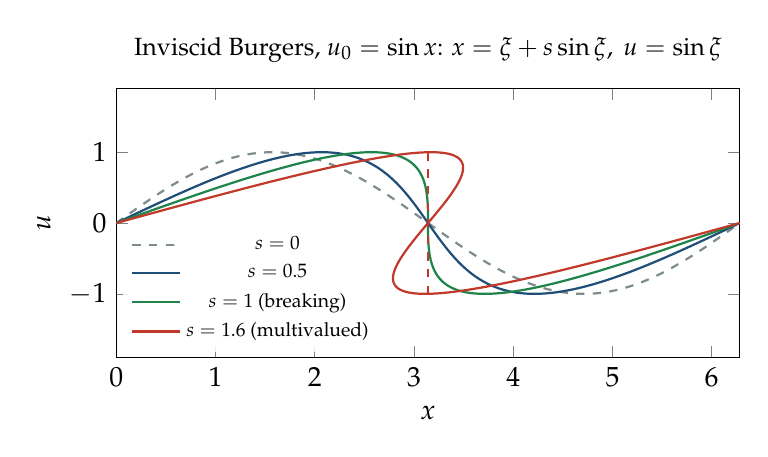
\begin{tikzpicture}
\begin{axis}[width=9.5cm,height=5.0cm,xlabel={$x$},ylabel={$u$},xmin=0,xmax=6.283,ymin=-1.9,ymax=1.9,
 legend style={font=\scriptsize,draw=none,fill=white,fill opacity=0.85,text opacity=1,at={(0.01,0.02)},anchor=south west},
 title={\small Inviscid Burgers, $u_0=\sin x$: $x=\xi+s\sin\xi,\ u=\sin\xi$},no markers,domain=0:6.283185,samples=200,smooth]
\addplot[cG,thick,dashed,variable=\z] ({\z},{sin(deg(\z))});
\addplot[cA,thick,variable=\z] ({\z+0.5*sin(deg(\z))},{sin(deg(\z))});
\addplot[cC,thick,variable=\z] ({\z+1.0*sin(deg(\z))},{sin(deg(\z))});
\addplot[cB,thick,variable=\z] ({\z+1.6*sin(deg(\z))},{sin(deg(\z))});
\draw[cB,dashed] (axis cs:3.14159,-1) -- (axis cs:3.14159,1);
\legend{$s=0$,$s=0.5$,$s=1$ (breaking),$s=1.6$ (multivalued)}
\end{axis}
\end{tikzpicture}
\caption{Characteristic solution of the inviscid flow of $-uu_x$. At $s=1$ the profile has a vertical tangent: the gradient blows up. Beyond that the curve folds; the physical (entropy) solution replaces the fold by a jump at $x=\pi$ (equal-area rule), shown dashed. This breaking is what makes $\Eint$ discontinuous after the shock.}\label{fig:burgers}
\end{figure}
\paragraph{Before the shock ($t<t^*$): smooth regime.} Smoothness permits perturbative expansions and derivative-based estimates.
\begin{itemize}[nosep]
\item $\Eint$ has a closed form at first order in $\nu$, with remainder $O(\nu^2\varepsilon^2t^3)$ \led{S4T-T2} \proved; it blows up at the breaking time $t^*$ \led{S4T-P3}. (This is the same family of expansions as Theorem~\ref{thm:jet} and Example~\ref{ex:burgers-jet}.)
\item The Cole--Hopf substitution $u=-2\nu\varphi_x/\varphi$ turns Burgers into the heat equation $\varphi_t=\nu\varphi_{xx}$; the inverse scattering transform linearizes KdV and NLS. These are used as the ``exact linearization'' of the nonlinear solution~\cite{ch}.
\end{itemize}
\paragraph{At breaking ($t=t^*$): estimates that need smoothness fail.} The inviscid gradient $u_x$ blows up (vertical tangent, $s=1$ in Figure~\ref{fig:burgers}), so every statement that needs bounds on $u_x,u_{xx},\dots$ stops being usable at $t^*$: the closed form of $\Eint$ blows up, and estimates that require smoothness, such as those behind the jet expansion of Theorem~\ref{thm:jet}, are no longer valid.
\paragraph{After the shock ($t>t^*$): discontinuous regime.}
The flow of $-uu_x$ alone forms a shock, so $\Eint$ jumps by amounts independent of $\nu$; this is forced by the definition. A function with a jump is not in $H^1$ in one dimension, so the Sobolev norms of Sections~\ref{sec:fact} and~\ref{sec:terms} are no longer the natural ones: pointwise values are unreliable, while the \emph{measure} of the discrepancy is well behaved. The meaningful quantities are therefore $L^1$ sizes, collected below:
\begin{align}
\|\Eint\|_{L^1}&=\Theta(\nu),\\
\sup_{t\le T}\|\Eint\|_{L^1}&=\nu|\log\nu|+O(\nu),\\
\|S-S_1S_2\|_{L^1}&=\Theta(\sqrt\nu).
\end{align}
The first line holds at fixed $t$, each shock contributing $4\nu\log\!\big(2\cosh(\rho/2)\big)$; the second has exact leading coefficient $1$. Sources: the first line is \led{OPA-T1} \modulo{Kru\v zkov uniqueness~\cite{kr}}; the second is \led{OPF5A-T1/T2}; the third is \led{OPF5D-T6} \proved.
The second line holds for data with a single birth of shock such as $\sin x$, and is conditional on a localization lemma in general \condl{}.

\begin{table}[!htb]
\centering\small
\begin{tabular}{@{}L{3.0cm}L{4.9cm}L{6.2cm}@{}}
\toprule
Regime & What happens & Tools and results\\\midrule
Before the shock, $t<t^*$ & the profile is smooth, characteristics do not cross & jet expansion (Thm.~\ref{thm:jet}), first-order closed form of $\Eint$, Cole--Hopf\\
At breaking, $t=t^*$ & the inviscid gradient blows up (vertical tangent) & smoothness-based estimates fail; $\Eint$ blows up\\
After the shock, $t>t^*$ & the single-term flow is discontinuous (equal-area rule) & $L^1$ estimates: $\Theta(\nu)$, $\nu|\log\nu|$, $\Theta(\sqrt\nu)$\\
\bottomrule
\end{tabular}
\caption{The three regimes of the Burgers interaction term and the tools that apply in each.}\label{tab:regimes}
\end{table}

%--- E13: Section 7.2, after the paragraph on the regimes / table ------------
\begin{explained}{Burgers: why the shock forms and what happens to the interaction}
\textbf{Step 1: why inviscid Burgers forms a shock.} $u_t+uu_x=0$ is nonlinear transport: the velocity at each point is $u$ itself. Along a characteristic starting at $x=\xi$, $dx/dt=u$ and $du/dt=0$, so $u$ stays constant, $u(x(t),t)=u_0(\xi)$. For $u_0=\sin\xi$:
\[
x=\xi+t\sin\xi,\qquad u=\sin\xi .
\]
Differentiating, $\partial x/\partial\xi=1+t\cos\xi$; as long as it is positive everywhere the map $\xi\mapsto x$ is invertible and the solution is smooth. It first vanishes when $1+t\cos\xi=0$; since $\min\cos=-1$, the breaking time is $t^*=1$ at $\xi^*=\pi$. The gradient $u_x=\dfrac{\cos\xi}{1+t\cos\xi}$ has numerator $\to-1$ and denominator $\to0$ at $(t,\xi)=(1,\pi)$, so it blows up. \emph{Before $t=1$} characteristics do not cross and there is one value of $u$ per $x$. \emph{At and after} $t=1$ they compress and cross, the parametric curve folds, no single-valued classical solution exists, and the entropy solution replaces the fold with a shock (for this symmetric datum at $x=\pi$).

\medskip\textbf{Step 2: where the interaction enters.} Viscous Burgers $u_t+uu_x=\nu u_{xx}$ is split into nonlinear transport $A_{\mathrm{tr}}u=-uu_x$ and diffusion $A_{\mathrm{diff}}u=\nu u_{xx}$. With $S(t)$ the full flow and $S_1,S_2$ the single-term flows,
\[
\Eint(t)=S(t)u_0-S_1(t)u_0-S_2(t)u_0+u_0 .
\]
Before the shock all flows can be compared with smooth expansions; after it, the transport flow develops a discontinuity while the viscous solution smooths the transition over a thin layer. That difference drives everything below.

\medskip\textbf{Step 3: why the smooth expansion breaks down.} Before breaking there is a first-order expansion in $\nu$ with remainder $O(\nu^2\varepsilon^2t^3)$ (the exact coefficient depends on the definitions of the paper; the parameter $\varepsilon$ is not defined in the text and is flagged in the author's notes). A perturbative expansion is useful while the relevant solutions stay smooth. At $t^*$ the inviscid gradient is unbounded and estimates relying on bounded derivatives fail. \emph{Precision:} what blows up at $t^*$ is the perturbative expression or its estimates, not the viscous solution itself, which stays finite because positive viscosity regularizes.

\medskip\textbf{Step 4: a jump that survives $\nu\to0$.} After the shock the transport flow is discontinuous while the viscous flow has a thin smooth layer. Even if the viscous profile converges to the entropy solution, the individual pieces of the difference need not converge so that their pointwise jumps cancel; hence $\Eint$ can have a jump of size independent of $\nu$. This does not contradict smallness in $L^1$: a function of amplitude $O(1)$ supported on an interval of width $O(\nu)$ has $\|E\|_{L^\infty}=O(1)$ but $\|E\|_{L^1}=O(\nu)$. The integral measures the area under $|E|$, not the maximum height.

\medskip\textbf{Step 5: the three estimates.}
\begin{center}\small
\begin{tabular}{@{}L{4.3cm}L{3.0cm}L{6.6cm}@{}}
\toprule
Quantity & Claimed scale & Interpretation\\\midrule
$\|\Eint(t)\|_{L^1}$ at fixed $t$ & $\Theta(\nu)$ & small in total absolute magnitude at a fixed post-shock time\\
$\sup_{t\le T}\|\Eint(t)\|_{L^1}$ & $\nu|\log\nu|+O(\nu)$ & the worst case over the time interval has a logarithmic enhancement\\
$\|S-S_1S_2\|_{L^1}$ & $\Theta(\sqrt\nu)$ & a different, larger scale: the error of replacing the full evolution by a composition of separate flows\\
\bottomrule
\end{tabular}
\end{center}
$\Theta(\nu)$ means bounded above and below by positive multiples of $\nu$ as $\nu\to0$. The third quantity is a different object: it concerns $S-S_1S_2$, not the additive remainder, and must not be conflated with it. Exact constants and rates depend on the definitions of the split flows, the domain and the theorem's hypotheses; the status labels in the text say what was proved and what is conditional.

\medskip\textbf{Step 6: the broader lesson.} Three regimes: before the shock, smoothness permits perturbative expansions and derivative-based estimates; at breaking, the inviscid gradient blows up and smoothness-based estimates fail; after the shock, pointwise behaviour can be discontinuous, so $L^1$ estimates become more informative than pointwise bounds. A nonlinear interaction can remain small in an integral norm even when its pointwise behaviour changes dramatically at shock formation.
\end{explained}



\subsection{Identification relative to a dictionary}
Nonlinear terms cannot be handled by the ideal $\Ann(u)$ of Section~\ref{sec:prelim}; instead one fixes a finite candidate list. Choose a dictionary $\mathcal D$ of monomials of degree $\le d$ in the jet, of order $\le k$, and ask which polynomial relations $F(u,u_x,\dots)=0$ the data satisfy. Notation: $V$ is the span of $\mathcal D$, $I(u)$ the ideal of all differential relations satisfied by $u$, $[F]$ the differential ideal generated by $F$, and $\mathcal J_u$ the jet-level obstruction (a different object from the cofactor $J_u$ of Section~\ref{sec:prelim}, hence the calligraphic letter)\edmark{E13}.
\begin{theorem}{(Dictionary criterion) \led{S4ID-T1} \proved[]}\label{thm:dict}
For smooth $u$ on any $\Omega$ there is an exact sequence $0\to[F]\cap V\to I(u)\cap V\to\mathcal J_u\cap\psi(V)\to0$. In particular
\[
I(u)\cap V=[F]\cap V\iff\mathcal J_u\cap\psi(V)=0 .
\]
\end{theorem}
The correct statement is therefore ``the relations are exactly $F$ \emph{modulo its differential consequences}''; the literal ``$I(u)\cap V=\langle F\rangle$'' is false in complete dictionaries (they contain $\partial_xF$, etc.) \led{S4ID-P1}. Concrete criteria: for Burgers with $N$ shocks, $u$ identifies the equation in the evolutionary dictionary iff $d\le N$ \led{S4ID-T2, OP-T7}; for $N$-soliton KdV the identifying polynomial has total degree $(N+2)2^{N-1}$ (generic $N=2$: $8$) \led{OP-K15} \modulo{Novikov 1974~\cite{no}}. Finally, ``closed form $\Rightarrow$ does not identify'' is itself a theorem \led{S4ID-T4}.
\edmark{E2}

%--- E14: Section 7.3, after the dictionary criterion ------------------------
\begin{explained}{identifying a nonlinear equation relative to a dictionary}
\textbf{Step 1: why $\Ann(u)$ is no longer enough.} For a linear equation, e.g.\ $u=e^{x-t}$, $(\partial_t+\partial_x)u=0$ is the action of a linear constant-coefficient operator. In $u_t+uu_x=0$ the term $uu_x$ multiplies two quantities depending on $u$: it is not the action of a linear constant-coefficient operator on $u$, so we need another language: polynomial expressions in the jet variables.

\medskip\textbf{Step 2: jets and the dictionary.} Fix a maximal order $k$ and take the jet variables $u,u_t,u_x,u_{tt},u_{tx},u_{xx},\dots$ up to order $k$. A polynomial in them is a candidate differential relation; Burgers is $F(u,u_t,u_x)=u_t+uu_x$. A \emph{dictionary} $\mathcal D$ is a finite list of candidate monomials, e.g.\ $\{u_t,u_x,u^2,uu_x,u_{xx},\dots\}$, and $V=\spn\mathcal D$ contains all linear combinations. A candidate equation is $c_1u_t+c_2uu_x+c_3u_{xx}=0$; identifying the equation from data means finding the coefficients for which the relation holds on the observed solution. $V$ is a finite-dimensional vector space of candidates, \emph{not} necessarily an ideal: the dictionary limits what one is willing to consider.

\medskip\textbf{Step 3: $I(u)$ versus $[F]$.} $I(u)$ is the differential ideal of \emph{all} polynomial differential relations satisfied by $u$. If $F=u_t+uu_x=0$ holds identically, so do its derivatives, e.g.\ $D_xF=u_{tx}+u_x^2+uu_{xx}$ (total derivative $D_x$). $[F]$, the differential ideal generated by $F$, contains $F$, its differential consequences $D_xF,D_tF,\dots$ and polynomial combinations of them. If $u$ solves $F=0$ then $[F]\subseteq I(u)$, but the inclusion can be strict: a particular solution may satisfy additional relations that do not follow from the equation alone. That is the core of identifiability.

\medskip\textbf{Step 4: why ``$I(u)\cap V=\langle F\rangle$'' is wrong.} If $\mathcal D$ contains the monomials of both $F$ and $D_xF$, both lie in $V$. If $\langle F\rangle$ meant only scalar multiples of $F$, it would not contain $D_xF$, which is certainly a relation satisfied by the solution. The correct comparison is
\[
I(u)\cap V=[F]\cap V:
\]
every relation of the dictionary that the data satisfy is already a differential consequence of the proposed equation. It does \emph{not} require the data to satisfy only the original equation and nothing derived from it.

\medskip\textbf{Step 5: the exact sequence.}
\[
0\to[F]\cap V\to I(u)\cap V\to\mathcal J_u\cap\psi(V)\to0 .
\]
$\mathcal J_u$ is the jet-level obstruction (distinct from the cofactor $J_u$ of Section~\ref{sec:prelim}) and $\psi$ the map from candidate expressions to jet-level objects (its precise definition is flagged in the author's notes). The first term holds the dictionary relations explained by the proposed equation, the middle term every dictionary relation the data satisfy, the last the extra relations left after quotienting out the consequences of $F$. Exactness gives $I(u)\cap V=[F]\cap V\iff\mathcal J_u\cap\psi(V)=\{0\}$: the dictionary contains no detectable obstruction. It is a \emph{finite-dictionary} criterion: it does not say the data identify the equation among all conceivable nonlinear PDEs, only relative to the chosen candidate space.

\medskip\textbf{Step 6: shocks and solitons.} Identifiability depends on the solution, not only on the equation. \emph{Burgers with $N$ shocks:} in the paper's evolutionary dictionary the equation is identified iff the maximal polynomial degree satisfies $d\le N$; shock structure gives information that distinguishes the equation from competing polynomial relations, depending on the number of shocks and on the allowed degree of candidate terms (specific to the dictionary and assumptions of the cited result). \emph{$N$-soliton KdV:} the identifying polynomial has total degree $(N+2)2^{N-1}$; for $N=2$ this is $(2+2)\cdot2^{1}=8$. A special solution can satisfy many polynomial relations, so a sufficiently rich dictionary is needed to reveal which relation actually identifies the equation rather than describing that particular solution.

\medskip\textbf{Step 7: why a closed form can fail to identify.} $u=e^{x+t}$ satisfies $u_t-u=0$, $u_x-u=0$, and consequences such as $u_{tx}-u=0$, $u_{xx}-u=0$. The solution alone does not say which relation is ``the'' governing equation: several equations explain the same special function. That is the intuition behind ``closed form $\Rightarrow$ does not identify''; the exact meaning of ``closed form'' in the theorem is the one fixed in the cited result, but the broad lesson is that an explicit solution may be too special to separate the true equation from competitors.

\medskip\textbf{The big picture.} The question changes from ``which linear differential operators annihilate $u$?'' to ``which polynomial differential relations does $u$ satisfy, and which genuinely identify its equation rather than merely describing a special solution?''. The dictionary makes the question finite-dimensional; $[F]$ accounts for all consequences of the proposed equation; $\mathcal J_u\cap\psi(V)$ detects extra relations. The crucial distinction is between \emph{fitting} a solution and \emph{identifying} its equation.
\end{explained}



\subsection{Linear versus nonlinear: the same idea, two structures}
Sections~\ref{sec:prelim}--\ref{sec:terms} and the present one answer the same question: \emph{what does a single solution $u$ remember about its equation?} In both settings we collect all relations satisfied by $u$ and ask when these relations are generated by the equation we were given. What changes is the algebraic structure in which the relations live.
\begin{table}[!htb]
\centering\small
\begin{tabular}{@{}L{2.8cm}L{6.2cm}L{6.2cm}@{}}
\toprule
 & Linear approach (Sections~\ref{sec:prelim}--\ref{sec:terms}) & Nonlinear approach (this section)\\\midrule
Space of candidate equations & the ring $\ring=\C[\tau,\xi]$ of constant-coefficient operators & a finite \emph{dictionary} $\mathcal D$ of jet monomials of degree $\le d$ and order $\le k$; $V=\spn\mathcal D$\\
Relations satisfied by $u$ & $\Ann(u)$, an ideal of $\ring$ & $I(u)$, the ideal of all differential relations\\
What the equation generates & the principal ideal $(P)$ & the differential ideal $[F]$\\
Criterion for identification & $\Ann(u)=(P)$ (Theorem~\ref{thm:ident}) & $I(u)\cap V=[F]\cap V$, i.e.\ $F$ \emph{modulo its differential consequences} (Theorem~\ref{thm:dict})\\
What escapes the equation & the cofactor $J_u$: the finitely many exponentials in $u$ ($\sigma_p(u)=\Var(J_u)$) & the jet-level obstruction $\mathcal J_u\cap\psi(V)$ (exact sequence of Theorem~\ref{thm:dict})\\
Solutions that do not identify & $u\in\EP$ & closed-form solutions (\led{S4ID-T4})\\
Concrete criteria & finite linear algebra (Lemma~\ref{lem:ep}) & Burgers with $N$ shocks identifies iff $d\le N$; $N$-soliton KdV: degree $(N+2)2^{N-1}$\\
\bottomrule
\end{tabular}
\caption{The linear and nonlinear identification problems side by side.}\label{tab:lin-nonlin}
\end{table}
\begin{aside}{Where the parallel breaks}
\textbf{Linear case.} The solutions form a vector space and the annihilators an ideal: one can add, multiply by operators and factor, which is why the Nullstellensatz applies and the test is a finite-dimensional computation.

\textbf{Nonlinear case.} There is no linear structure on the solutions: one must fix a finite space $V$ of candidates in advance, and the identification is \emph{relative to $V$}, never absolute. The literal statement
\[
I(u)\cap V=\langle F\rangle
\]
is false in complete dictionaries, which contain $\partial_xF$, so the correct statement is ``modulo differential consequences''.
\end{aside}

%--- E15: Section 7.4, comment on the two approaches ------------------------
\begin{explained}{future comments: the linear and the nonlinear approach compared}
You are not identifying the \emph{functions}; you are identifying the \emph{equations or relations} that the observed functions satisfy. Both approaches share this philosophy but use different mathematical objects.

\medskip\textbf{Linear case: look for an annihilating operator.} Given an observed $u(t,x)$ one searches for a constant-coefficient operator with $P(\partial_t,\partial_x)u=0$. For $u=e^{x+t}$: $(\partial_t-1)u=0$ and $(\partial_x-1)u=0$. One studies $\Ann(u)=\{P\in\C[\partial_t,\partial_x]:Pu=0\}$ and wants to characterize all the linear operators that annihilate $u$.

\medskip\textbf{Nonlinear case: search inside a finite dictionary.} For Burgers' $u_t+uu_x=0$ the product $uu_x$ is not a linear constant-coefficient operator applied to $u$. One chooses a finite dictionary, e.g.\ $\mathcal D=\{u_t,u_x,uu_x,u_{xx},u^2\}$, and searches for coefficients, not all zero, such that $c_1u_t+c_2u_x+c_3uu_x+c_4u_{xx}+c_5u^2=0$. This is a \emph{linear-algebra} problem in the unknown coefficients even though the candidate terms are nonlinear functions of $u$. If the data satisfy Burgers the coefficient vector $(1,0,1,0,0)$ works. The dictionary can be enlarged (higher-degree products, higher-order derivatives) but its limits must be decided in advance.

\medskip\textbf{What stays and what changes.}
\begin{center}\small
\begin{tabular}{@{}L{2.9cm}L{5.6cm}L{5.8cm}@{}}
\toprule
 & Linear approach & Nonlinear approach\\\midrule
Object observed & the function $u$ & the function $u$\\
Candidate relations & linear differential operators & differential polynomials\\
Search space & polynomial ring of constant-coefficient operators & a chosen finite dictionary of jet monomials\\
Main question & which operators annihilate $u$? & which candidate relations does $u$ satisfy?\\
Main limitation & structure of the annihilator & the dictionary may omit the true equation or contain too few informative terms\\
\bottomrule
\end{tabular}
\end{center}
The common principle is \emph{identifiability}: does the observed data contain enough information to distinguish the governing equation from alternative candidates?

\medskip\textbf{Where components and interactions enter.} For $u=u_1+u_2$ one can look at the components, the total, and an interaction term such as $\Eint=u-u_0-(u_1-u_0)-(u_2-u_0)$ (the additive form of Section~\ref{sec:terms}). \emph{Decomposition and interaction analysis} ask how the solution is assembled and how its components influence one another; \emph{equation identification} asks which differential relation governs the observed solution or its components. A linear annihilator may be used for a component when the assumptions allow, and a nonlinear dictionary to identify a nonlinear equation governing the total solution: complementary analyses, not automatically the same procedure.

\medskip\textbf{Key point.} The nonlinear dictionary approach generalizes the identification philosophy; it is not a direct replacement for the annihilator in every mathematical sense. The dictionary makes the search computationally manageable, but it also limits what can be discovered.
\end{explained}



\begin{keypoint}
Both approaches ask what one solution determines about its equation. The linear one answers with the annihilator ideal $\Ann(u)$ and its generator $G_u$; the nonlinear one answers with a dictionary and the differential ideal of relations, and only up to differential consequences. In the algorithm (Section~\ref{sec:algo}) Steps~1--6 use the structure of $\Ann(u)$, while Step~7 switches to the dictionary and returns a relative identification.
\end{keypoint}

%======================================================================
\section{The algorithm}\label{sec:algo}
\sectionbrief
{input of one of the data models M1--M3 below, and for each step the hypotheses of the theorem that justifies it.}
{to turn the theorems into one procedure with explicit inputs, outputs, and guarantees.}
{operational summary of Sections~\ref{sec:ident}--\ref{sec:nonlin}. Table~\ref{tab:steps} lists the steps, Figure~\ref{fig:algo} the control flow, and a worked example makes them concrete.}

\subsection{Inputs and data models}
The reconstruction is exact, hence the input must be of an exact kind. Three data models were analysed \led{O7}:
\begin{description}[nosep,leftmargin=2.2cm,labelwidth=2cm]
\item[M1] closed-form $u$ (e.g.\ sums of exponentials and Gaussians);
\item[M2] the jet of $u$ at a point, to a given order;
\item[M3] $u$ real-analytic on a connected $\Omega$, given through a holonomic ideal with coefficients in $\overline{\mathbb Q}$ (assumption (AC) on computing jets).
\end{description}
In model M1 the integral-ring identification never holds \led{C3-C2}, and relative identification is used.

\subsection{The pipeline}
\begin{center}
\small
\begin{tabular}{@{}c L{2.7cm} L{4.9cm} L{5.6cm}@{}}
\toprule
Step & Task & Result relied upon & Output\\\midrule
0 & Input & data models M1--M3 & exact $u$\\
1 & Annihilator & jet Gram matrix kernel & candidate $P$\\
2 & Factor & unique factorization (F1) & irreducible factors $P_i$, $e_i$\\
3 & EP test & Lemma~\ref{lem:ep}, Thm.~\ref{thm:ident} & verdict per factor\\
4 & Reduce & Prop.~\ref{prop:spec}, ledger C3-T6 & $G_u$, $J_u$, certificate\\
5 & Decompose & Thm.~\ref{thm:factor}, Eq.~\eqref{eq:lagrange} & components $u_j$, ambiguity $\delta(P)$\\
6 & Terms & Thm.~\ref{thm:eint} & log-symbol, $\Eint$\\
7 & Nonlinear branch & Thm.~\ref{thm:dict}, Sec.~\ref{sec:nonlin} & relative identification, flow-based $\Eint$\\
\bottomrule
\end{tabular}
\captionof{table}{The steps of the algorithm at a glance: what each step does, which result justifies it, and what it returns.}\label{tab:steps}
\end{center}
\begin{figure}[!htb]
\centering
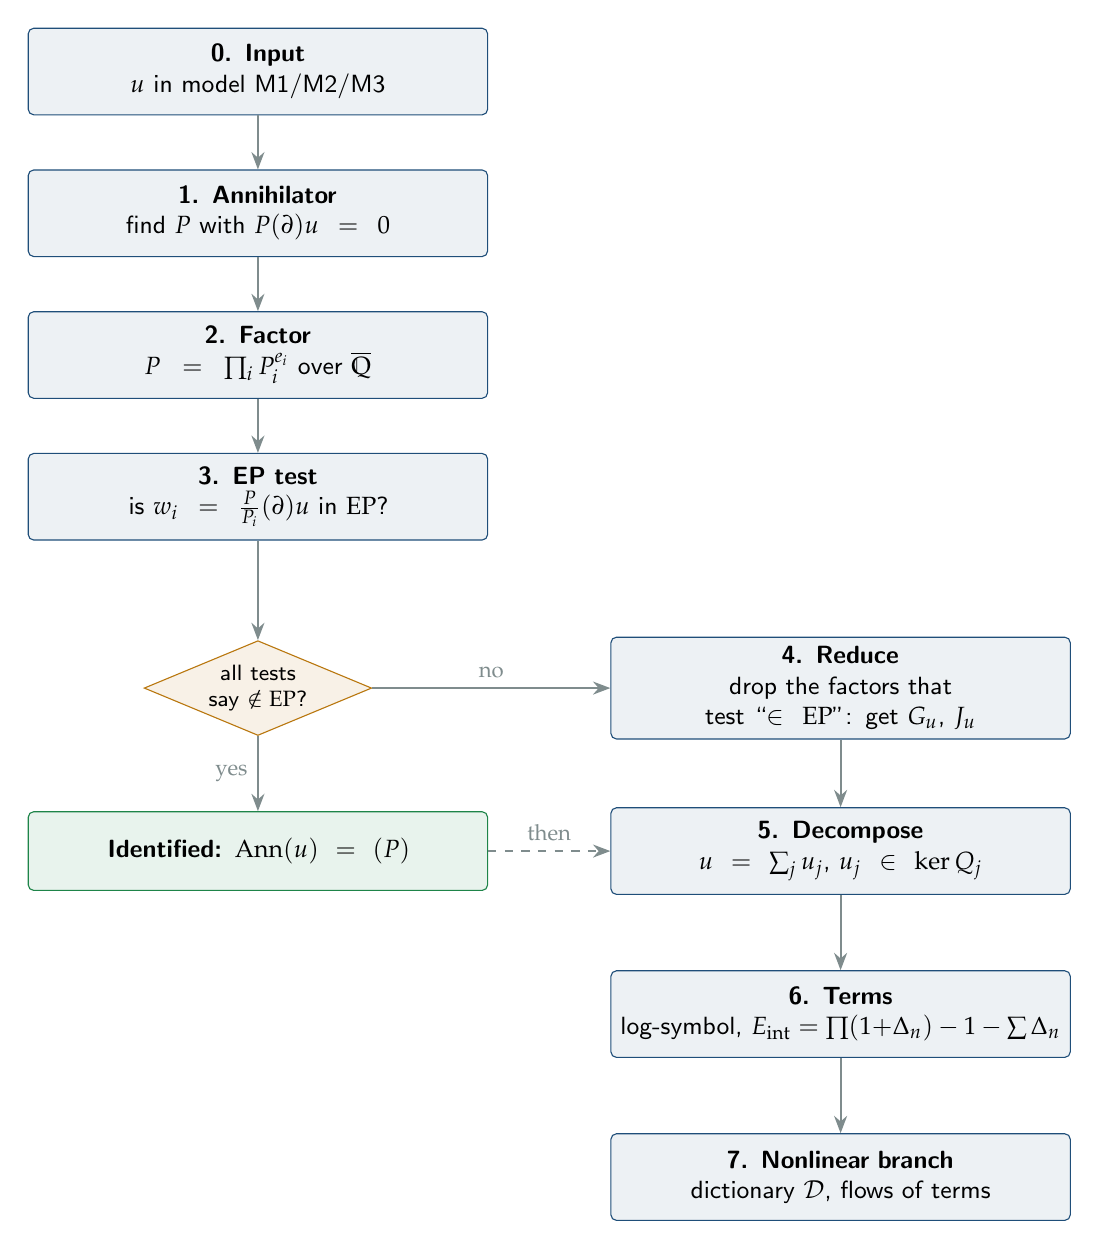
\begin{tikzpicture}[
  st/.style={draw=cA,fill=cA!8,rounded corners=2pt,minimum height=11mm,text width=5.6cm,align=center,font=\small\sffamily},
  dec/.style={draw=cD,fill=cD!10,diamond,aspect=2.4,inner sep=1pt,align=center,font=\footnotesize\sffamily},
  outb/.style={draw=cC,fill=cC!10,rounded corners=2pt,minimum height=10mm,text width=5.6cm,align=center,font=\small\sffamily},
  arr/.style={-{Stealth[length=2.2mm]},thick,cG}]
\def\dy{1.8}
\node[st] (s0) at (0,0) {\textbf{0. Input}\\ $u$ in model M1/M2/M3};
\node[st] (s1) at (0,-\dy) {\textbf{1. Annihilator}\\ find $P$ with $P(\partial)u=0$};
\node[st] (s2) at (0,-2*\dy) {\textbf{2. Factor}\\ $P=\prod_iP_i^{e_i}$ over $\overline{\mathbb Q}$};
\node[st] (s3) at (0,-3*\dy) {\textbf{3. EP test}\\ is $w_i=\tfrac{P}{P_i}(\partial)u$ in $\EP$?};
\node[dec] (d) at (0,-4.35*\dy) {all tests\\ say $\notin\EP$?};
\node[outb] (o1) at (0,-5.5*\dy) {\textbf{Identified:} $\Ann(u)=(P)$};
\node[st] (s4) at (7.4,-4.35*\dy) {\textbf{4. Reduce}\\ drop the factors that test ``$\in\EP$'': get $G_u$, $J_u$};
\node[st] (s5) at (7.4,-5.5*\dy) {\textbf{5. Decompose}\\ $u=\sum_ju_j$, $u_j\in\ker Q_j$};
\node[st] (s6) at (7.4,-6.65*\dy) {\textbf{6. Terms}\\ log-symbol, $\Eint=\prod(1{+}\Delta_n)-1-\sum\Delta_n$};
\node[st] (s7) at (7.4,-7.8*\dy) {\textbf{7. Nonlinear branch}\\ dictionary $\mathcal D$, flows of terms};
\draw[arr] (s0)--(s1); \draw[arr] (s1)--(s2); \draw[arr] (s2)--(s3); \draw[arr] (s3)--(d);
\draw[arr] (d)--node[left,font=\footnotesize]{yes}(o1);
\draw[arr] (d)--node[above,font=\footnotesize]{no}(s4);
\draw[arr] (s4)--(s5); \draw[arr] (s5)--(s6); \draw[arr] (s6)--(s7);
\draw[arr,dashed] (o1)--node[above,font=\footnotesize]{then}(s5);
\end{tikzpicture}
\caption{The algorithm as a flowchart. Left column: steps 0--3 certify what the operator is. If every factor test fails (no leftover is an exponential-polynomial) the operator is identified; otherwise step~4 reduces it to $G_u$. Right column: steps 4--7 extract structure from $u$ once the operator is known; the dashed arrow shows that an identified operator proceeds directly to decomposition.}\label{fig:algo}
\end{figure}

\subsection{The steps in detail}
\stepblock{1}{obtain an annihilator}
\begin{description}[nosep,leftmargin=2.6cm,labelwidth=2.4cm]
\item[Does] Let $\Phi(u)=(T_1u,\dots,T_Mu)^{\top}$ be the jet over a dictionary of $M$ candidate terms and $\mathbb G(u)=\int_\Omega\Phi\Phi^{*}\dd\mu$ its Gram matrix (positive semidefinite). A relation $\lambda\cdot\Phi=0$ holds iff $\lambda\in\ker\mathbb G(u)$.
\item[How] Exact arithmetic (rational or algebraic coefficients), Gaussian elimination: no learning, no statistics.
\item[Returns] a candidate $P$. If $\ker\mathbb G$ has dimension $>1$, $u$ satisfies several dictionary relations, which is itself information about $G_u$ and $J_u$.
\end{description}
\edmark{E3}

\stepblock{2}{factor}
\begin{description}[nosep,leftmargin=2.6cm,labelwidth=2.4cm]
\item[Does] factor $P(\tau,\xi)\in\overline{\mathbb Q}[\tau,\xi]$ into irreducibles with multiplicities (a standard computer-algebra operation).
\item[Returns] the factors $P_i$ and exponents $e_i$.
\end{description}

\stepblock{3}{exponential-polynomial test}
\begin{description}[nosep,leftmargin=2.6cm,labelwidth=2.4cm]
\item[Does] for each $i$ compute $w_i=(P/P_i)(\partial)u$ and decide whether $\dimc\ring w_i<\infty$; by Theorem~\ref{thm:ident}(a) this is exactly the identification test.
\item[How] depends on the data model:
 \begin{itemize}[nosep]
 \item M1: a syntactic check (is the closed form a finite sum of polynomials times exponentials?);
 \item M3: a Gr\"obner basis of the holonomic annihilator, checking for finite holonomic rank in the sense of Lemma~\ref{lem:ep} \led{OP-ALG-T1};
 \item M2: undecidable from the jet alone \led{P4-T5}; one needs an upper bound $B\ge\dimc(\ring u\cap\EP)$, after which comparing the first $B$ derivatives suffices \led{P4-T4}.
 \end{itemize}
\end{description}

\stepblock{4}{reduce to $G_u$}
\begin{description}[nosep,leftmargin=2.6cm,labelwidth=2.4cm]
\item[Does] drop from $P$ every factor $P_i$ whose test returned ``EP'' (with the correct multiplicity bookkeeping: at most $\sum_ie_i$ tests in total \led{C3-T6}).
\item[Returns] $G_u$, the intrinsic operator; the dropped part is $J_u$, whose finite zero set is the point spectrum (the exponentials contained in $u$). Certificate: ``$\Ann(u)=(P)$'' if nothing was dropped, else ``$u$ identifies only $G_u$ and contains these exponentials''.
\end{description}

\stepblock{5}{decompose}
\begin{description}[nosep,leftmargin=2.6cm,labelwidth=2.4cm]
\item[Evolution factors] $\tau-a_j(\xi)$: apply \eqref{eq:lagrange}.
\item[General coprime factors] use the exact-sequence construction of Theorem~\ref{thm:factor}; the components are determined up to the finite exponential-polynomial space of dimension $\delta(P)$, fixed by a normalization (for the wave equation, by fixing the constant, Example~\ref{ex:wave}).
\item[Check] before using the components in $H^m$, verify $\gamma_N>0$ (Theorem~\ref{thm:hm}).
\end{description}

\stepblock{6}{terms and interaction}
\begin{description}[nosep,leftmargin=2.6cm,labelwidth=2.4cm]
\item[Does] inside an evolution factor with symbol $a(\xi)=\sum_na_n(\xi)$, read the terms as the coefficients of $\log\hat u(t,\kappa)=t\sum_na_n(\kappa)+\log\hat u_0(\kappa)$ (linear in the terms, cost $O(N)$); evaluate $\Eint$ by \eqref{eq:eint}.
\item[Non-commuting] classify the generated Lie algebra: solvable $\Rightarrow$ exact formula; otherwise a local expansion only.
\end{description}

\stepblock{7}{nonlinear case}
Replace Step~3 by the dictionary criterion of Theorem~\ref{thm:dict} and Step~6 by the flow-based $\Eint$ of Section~\ref{sec:nonlin}.

\subsection{Worked example}
We follow Steps 1--6 on the wave equation with $c=1$ and the (non-exponential) solution
\[
u(t,x)=\underbrace{\frac{1}{1+(x+t)^2}}_{f(x+t)}+\underbrace{e^{-(x-t)^2}}_{g(x-t)} .
\]
Each box below states the goal, the computation, and the outcome of one step.

\begin{wstep}{Step 1 --- annihilator}
\textbf{Goal.} Find an equation satisfied by $u$.\\
\textbf{Computation.} Take the dictionary $\{u_{tt},u_{xx},u_{tx},u_t,u_x,u\}$; the relations $\lambda\cdot\Phi=0$ form the line spanned by $u_{tt}-u_{xx}=0$.\\
\textbf{Outcome.} $P=\tau^2-\xi^2$.
\end{wstep}

\begin{wstep}{Step 2 --- factor}
\textbf{Computation.}
\[
P=Q_1Q_2,\qquad Q_1=\tau-\xi,\quad Q_2=\tau+\xi .
\]
\textbf{Outcome.} Two irreducible, simple factors.
\end{wstep}

\begin{wstep}{Step 3 --- EP test, factor $Q_2$ removed}
\textbf{Goal.} Decide whether $w_1=Q_2(\partial)u=(\partial_t+\partial_x)u$ is an exponential-polynomial.\\
\textbf{Computation.} The two parts behave differently:
\[
(\partial_t+\partial_x)f(x+t)=2f'(x+t),\qquad (\partial_t+\partial_x)g(x-t)=-g'+g'=0 .
\]
With $f(s)=\dfrac1{1+s^2}$ one has $f'(s)=-\dfrac{2s}{(1+s^2)^2}$, hence
\[
w_1=2f'(x+t)=-\frac{4(x+t)}{\big(1+(x+t)^2\big)^2}.
\]
\textbf{Outcome.} $w_1$ is rational, not a finite sum of polynomials times exponentials, so $w_1\notin\EP$.
\end{wstep}

\begin{wstep}{Step 3 --- EP test, factor $Q_1$ removed}
\textbf{Computation.} Symmetrically, with $g(s)=e^{-s^2}$, $g'(s)=-2se^{-s^2}$:
\[
w_2=Q_1(\partial)u=(\partial_t-\partial_x)u=-2g'(x-t)=4(x-t)\,e^{-(x-t)^2}.
\]
\textbf{Outcome.} $w_2\notin\EP$ (a Gaussian times a polynomial is not an exponential-polynomial).
\end{wstep}

\begin{wstep}{Step 4 --- reduce}
\textbf{Outcome.} Both tests say $\notin\EP$, so nothing is dropped: $\Ann(u)=(\tau^2-\xi^2)$, the point spectrum is empty, and the wave equation is identified.
\end{wstep}

\begin{wstep}{Step 5 --- decompose}
\textbf{Computation.} $(Q_1,Q_2)=(\tau,\xi)$, so $\delta(P)=1$.\\
\textbf{Outcome.} The components are $u_1=f(x+t)$, recovered from $w_1$ by integration in $x$ at fixed $t$ up to a constant, and $u_2=g(x-t)$; they are determined up to a constant $k$ with $u_1+u_2$ fixed. Whether such components lie in $H^m$ for every solution is governed by Theorem~\ref{thm:hm} and is not asserted here.
\end{wstep}

\begin{wstep}{Step 6 --- terms}
Not applicable to the wave equation (no evolution factor with several terms). For the advection--diffusion case of Figure~\ref{fig:eint}, the log-symbol is
\[
\log\hat u(t,\kappa)=\log\hat u_0(\kappa)+t\,(-ic\kappa-D\kappa^2),
\]
its two coefficients are the two terms, and $\Eint$ follows from \eqref{eq:eint} at cost $O(N)=O(2)$ per point.
\end{wstep}

\subsection{Complexity summary}
Table~\ref{tab:complexity} collects the cost and feasibility of each component.
\begin{table}[!htb]
\centering
\small
\begin{tabular}{@{}lll@{}}
\toprule
Component & Cost / feasibility & Source\\\midrule
Annihilator from a dictionary & Gaussian elimination, $O(M^3)$ & Step 1\\
Factorization & standard computer-algebra operation & Step 2\\
EP test (M1) & syntactic & Step 3\\
EP test (M3) & Gr\"obner/holonomic, decidable mod (AC) & \led{OP-ALG-T1}\\
EP test (M2, black box) & impossible without a bound & \led{P4-T5}\\
Components (evolution) & one rational Fourier multiplier per factor & \eqref{eq:lagrange}\\
$\Eint$ value / by order / full table & $O(N)$ / $O(N^2)$ / $\Theta(2^N)$ & \led{P1-T3}\\
\bottomrule
\end{tabular}
\caption{Cost and feasibility of the algorithm's components.}\label{tab:complexity}
\end{table}

%======================================================================
\section{Limits, open problems, and status}\label{sec:limits}
\sectionbrief
{no new assumptions.}
{to state what is impossible, what is open, and how reliable the results are.}
{delimits the claims of the paper; Appendix~\ref{app:scope} compares the paper with the full research.}
\paragraph{What is impossible} (all \proved).
\begin{itemize}[nosep]
\item finite certificates of identification, and black-box identification (Section~\ref{sec:ident-limits});
\item per-term decomposition of the solution (Proposition~\ref{prop:terms}\edmark{E9});
\item stable regularization of $\Eint$ (Proposition~\ref{prop:discont});
\item identification by restricting variable-coefficient operators to one solution;
\item decomposition on domains with holes (Figure~\ref{fig:hole});
\item a finite product of single-term flows reproducing non-commuting dynamics.
\end{itemize}

\paragraph{Open or conditional.}
\begin{itemize}[nosep]
\item identification for analytic KdV data with nonzero reflection coefficient \led{INT-Q1} \openq;
\item time-uniform shock estimate with several shock births \led{OPA-Q1} \condl;
\item density of the sum of kernels on nonconvex domains \openq;
\item exact values $\delta_N(K)$ of an invariant for general $N$ \led{OPF5C-Q1} \openq;
\item nonlinear asymptotics with derivatives \led{S4ID-P8} \condl;
\item closedness of the sum of kernels for $N\ge3$ differential factors \led{C12-Q2} \openq.
\end{itemize}

\paragraph{Honest assessment.} Many ingredients are classical (Malgrange--Ehrenpreis, Nullstellensatz, Cole--Hopf, inverse scattering). The contribution is the \emph{package}: sharp characterizations, negative theorems, and counterexamples, each with a verified status. Independent reviewers were AI agents. Fifteen theorems of the algebraic core (the $\Eint$ identity for commuting flows, the comaximal factor decomposition with explicit projector, companion normality for $k=2$, irreducibility results) are formalized in Lean~4/Mathlib without \texttt{sorry}; the analytic parts (distributions, Sobolev spaces, semigroups) are not, since Mathlib lacks the libraries. Several citations were verified only on secondary sources; a result relied upon should be traced to its primary source. Out of scope so far: a variable potential treated as noise (Schr\"odinger/Dirac), matrix-valued coefficients ($4\times4$ Dirac), and any statistical preprocessing.

%======================================================================
%--- E16: Section 9, simple explanation of the last part ---------------------
\begin{explained}{the last section in plain words}
This section answers three simple questions: what can we \emph{never} do with this method, what do we \emph{not know yet}, and how much can we trust what is written.

\medskip\textbf{1. What is impossible.} These are proved facts, not gaps:
\begin{itemize}[nosep]
\item \emph{No finite proof of identification.} If $u$ is not an exponential-polynomial, no finite list of numbers (derivatives at a point, samples) can prove that $\Ann(u)=(P)$, because every finite list can also come from some exponential-polynomial. Example: you can refute ``$u$ is a sum of exponentials'' by finding a derivative that breaks it, but you can never confirm the opposite from finite data.
\item \emph{No splitting by terms.} Writing the solution as one piece per term of the operator fails: for the wave equation $\partial_t^2-c^2\partial_x^2$ only polynomial solutions split that way (Section~\ref{sec:fact}).
\item \emph{No stable removal of the interaction.} The interaction term cannot be switched off by a penalty or a regularization.
\item \emph{No identification with variable coefficients from one solution.}
\item \emph{No splitting on domains with a hole} (the logarithm example).
\item \emph{No finite product of single-term flows} reproduces non-commuting dynamics.
\end{itemize}

\medskip\textbf{2. What is open or conditional.} These are questions the paper cannot answer: KdV data with nonzero reflection coefficient; shock estimates uniform in time with several shock births; density of the sum of kernels on non-convex domains; exact values of an invariant $\delta_N(K)$; nonlinear asymptotics with derivatives; closedness of the sum of kernels for three or more differential factors. ``Open'' means unknown; ``conditional'' means true if an extra lemma holds.

\medskip\textbf{3. How reliable is it.} The paper is honest about this: many ingredients are classical (Nullstellensatz, Malgrange--Ehrenpreis, Cole--Hopf); the novelty is the \emph{package} of sharp statements, negative theorems and counterexamples, each with a status label. The reviewers were AI agents, not human referees; fifteen algebraic theorems were also machine-checked in Lean~4, while the analytic parts (distributions, Sobolev spaces, semigroups) were not, because the library is missing. Some citations were checked only on secondary sources, so before relying on a result one should trace it to its primary source.

\medskip\textbf{Take-home message.} Read the labels: \emph{proved} can be used, \emph{conditional} needs an extra lemma, \emph{open} is unknown, \emph{false} is a counterexample. The method is exact and has precise limits.
\end{explained}


\clearpage
\appendix
\section{Glossary of tools}\label{app:gloss}
Each entry states a classical tool in one sentence and points to the section where the paper uses it.
\begin{center}\small
\begin{tabular}{@{}L{3.4cm}L{9.2cm}L{2.0cm}@{}}
\toprule
Name & Statement in one sentence & Used in\\\midrule
Chinese remainder theorem & Coprime moduli split a quotient ring into a product; the algebra behind Thm.~\ref{thm:factor}. & Sec.~\ref{sec:fact}\\
Hilbert's Nullstellensatz & A polynomial vanishing on $\Var(I)$ has a power in $I$. & Sec.~\ref{sec:prelim}, \ref{sec:ident}\\
B\'ezout's theorem & Curves without common component meet in finitely many points (at most the product of degrees)~\cite{fu}. & Sec.~\ref{sec:prelim}\\
Malgrange--Ehrenpreis & Every nonzero constant-coefficient operator has a fundamental solution; $P(\partial)$ is onto on $C^\infty$ of a convex set~\cite{eh,ma}. & Sec.~\ref{sec:fact}\\
Ehrenpreis--Palamodov & Solutions of constant-coefficient systems are integrals of exponential-polynomial solutions over $\Var(P)$ (discrete sums when the spectrum is finite)~\cite{pa}. & context only\\
Friedrichs angle & $M+N$ is closed iff the cosine of the angle between $M\ominus(M\cap N)$ and $N\ominus(M\cap N)$ is $<1$. & Sec.~\ref{sec:fact}\\
Miyadera--Voigt & Small relatively bounded perturbations of a semigroup generator generate a semigroup; basis of \eqref{eq:dyson}~\cite{en}. & Sec.~\ref{sec:terms}\\
Baker--Campbell--Hausdorff & $e^Xe^Y=e^{X+Y+\frac12[X,Y]+\cdots}$. & Sec.~\ref{sec:terms}\\
Wei--Norman & Linear time-dependent systems on a solvable Lie algebra reduce to ODEs for scalar coefficients. & Sec.~\ref{sec:terms}\\
Cole--Hopf & $u=-2\nu\varphi_x/\varphi$ maps Burgers to the heat equation~\cite{ch}. & Sec.~\ref{sec:nonlin}\\
Kru\v zkov & Uniqueness and stability of entropy solutions of scalar conservation laws; defines the flow of $-uu_x$ after the shock~\cite{kr}. & Sec.~\ref{sec:nonlin}\\
Inverse scattering (IST) & KdV/NLS are linearized by a nonlinear Fourier transform with trivial time evolution. & Sec.~\ref{sec:nonlin}\\
\bottomrule
\end{tabular}
\end{center}

\section{Primer for readers new to the concepts}\label{app:primer}
This appendix \emph{adds} concrete explanations; nothing in the main text depends on reading it. It covers four notions in this order: ideals and annihilators (\S B.1), exponential-polynomials (\S B.2), the Chinese remainder theorem (\S B.3), and the companion matrix on a numerical example (\S B.4).

\subsection*{B.1 Ideals, annihilators and the gcd, starting from integers}
\paragraph{Integers.} The multiples of $6$ form an \emph{ideal} $(6)=\{\dots,-6,0,6,12,\dots\}$: it is closed under addition and under multiplication by any integer. The ideal generated by $4$ and $6$ is $(4,6)=(2)$, since $2=6-4$ and every combination is even: the ideal ``remembers'' only the $\gcd$.

\paragraph{Operators.} Replace integers by operators and ``multiple of $6$'' by ``kills $u$''. For $u=e^{x}$ every operator $Q(\partial_x)$ with $Q(1)=0$ kills $u$, i.e.\ every multiple of $\partial_x-1$. So
\[
\begin{aligned}
\Ann(e^x)&=(\partial_x-1),\\
\Ann(\sin x)&=(\partial_x^2+1),\\
\Ann(xe^x)&=\big((\partial_x-1)^2\big),\\
\Ann(e^x+e^{2x})&=\big((\partial_x-1)(\partial_x-2)\big).
\end{aligned}
\]
In one variable every annihilator ideal has a single generator (the \emph{minimal annihilator}), exactly as every ideal of integers is $(n)$. In two variables an ideal can need several generators, as $(\tau-\tau_0,\xi-\xi_0)$ does for $u=e^{\tau_0t+\xi_0x}$.

\paragraph{The gcd.} $\Ann(u)=G_uJ_u$ separates the part of the ideal that is a single polynomial multiple ($G_u$, ``infinite part'') from the part $J_u$ that has only finitely many common zeros ($J_u$, ``finite debris''). Example: for $u=f(x+t)$ with $f$ generic (not an exponential-polynomial), $\Ann(u)=(\partial_t-\partial_x)$ by Theorem~\ref{thm:ident}, so $G_u=\tau-\xi$ and $J_u=\ring$; for $u=e^{x+t}$, $\Ann(u)=(\tau-1,\xi-1)$, so $G_u=1$ and $J_u=\Ann(u)$.

\subsection*{B.2 Exponential-polynomials: examples and a test}
\begin{center}\small
\begin{tabular}{@{}L{5.4cm}L{2.3cm}L{6.8cm}@{}}
\toprule
Function & In $\EP$? & Reason (derivatives of $u$ span ...)\\\midrule
$xe^{x}$ & yes & $\spn\{xe^x,e^x\}$, dimension $2$\\
$x^2e^{3t}+\cos x$ & yes & finite sum of polynomial $\times$ exponential ($\cos x=\tfrac12(e^{ix}+e^{-ix})$)\\
$e^{-x^2}$ (Gaussian) & no & $\frac{d^k}{dx^k}e^{-x^2}=(\text{polynomial of degree }k)\,e^{-x^2}$: independent for all $k$, infinite dimension\\
$1/(1+x^2)$ & no & derivatives are rational functions with growing denominators: infinite dimension\\
\bottomrule
\end{tabular}
\end{center}
This is Lemma~\ref{lem:ep} in action: ``$u\in\EP$'' means ``its derivatives span a finite-dimensional space''.

\subsection*{B.3 The Chinese remainder theorem, concretely}
\paragraph{Integers.} The system $x\equiv1\pmod2$, $x\equiv2\pmod3$ has the unique solution $x\equiv5\pmod6$: $\Z/6\cong\Z/2\times\Z/3$. Coprimality of $2$ and $3$ is what makes the pair of remainders determine $x$.

\paragraph{One-variable ODE.} Let $p(\partial)=(\partial-1)(\partial-2)$. Then $\ker p=\ker(\partial-1)\oplus\ker(\partial-2)=\spn\{e^x,e^{2x}\}$, and the Lagrange-type projectors are explicit: if $u=ae^x+be^{2x}$,
\[
\begin{aligned}
u_1&=\frac{\partial-2}{1-2}\,u=\;\;a\,e^{x},\\
u_2&=\frac{\partial-1}{2-1}\,u=\;\;b\,e^{2x}.
\end{aligned}
\]
This is Eq.~\eqref{eq:lagrange} with $\partial_t$ replaced by $\partial$.

\paragraph{Two variables.} For the wave equation $Q_1=\tau-\xi$, $Q_2=\tau+\xi$ are coprime, but the ideal $(Q_1,Q_2)=(\tau,\xi)$ is not the unit ideal: the two lines meet at the origin. The quotient $\ring/(\tau,\xi)=\C$ has dimension $1$, which is the constant ambiguity $\delta(P)=1$ of Example~\ref{ex:wave}. Theorem~\ref{thm:factor} says that this finite overlap is the \emph{only} failure of the integer picture.

\subsection*{B.4 The companion matrix on a numerical example}
For $u''-3u'+2u=0$ the companion matrix is $C=\begin{pmatrix}0&1\\-2&3\end{pmatrix}$, with characteristic polynomial $\lambda^2-3\lambda+2$ and eigenvalues $1,2$. The projectors of Eq.~\eqref{eq:spectral} are $\Pi_1=\dfrac{C-2\Id}{1-2}$ and $\Pi_2=\dfrac{C-\Id}{2-1}$, and $e^{xC}=e^x\Pi_1+e^{2x}\Pi_2$.

\section{Scope: what this paper contains and what it does not}\label{app:scope}
This paper summarizes the research reported in \texttt{REPORT\_FINALE.md} (Phases 0--5). The following table compares it with the full project.
\begin{center}\small
\begin{tabular}{@{}L{4.4cm}L{5.6cm}L{4.6cm}@{}}
\toprule
Area & In this paper & Not in this paper\\\midrule
Linear identification & criterion, spectral form, limits (Sec.~\ref{sec:ident}) & proofs of the converse direction; details of OP-ALG and variable-coefficient classification\\
Factor decomposition & Thm.~\ref{thm:factor}, holes, Sobolev regularity (Sec.~\ref{sec:fact}) & the explicit $\delta_N(K)$ values (open), the cohomological criterion in detail\\
Terms and $\Eint$ & product formula, cost, instability, Dyson, Lie dichotomy (Sec.~\ref{sec:terms}) & boundary asymptotics beyond the stated rate; the balance decomposition\\
Nonlinear & Burgers asymptotics, dictionary criterion (Sec.~\ref{sec:nonlin}) & KdV/NLS scattering identification (INT-T1/T2), Hirota $N$-solitons, analyticity radius, KdV--Burgers remainder\\
Catalogue of kernels & -- & the catalogue of $\sim$60 equation types (C2), the tropical scaling reading\\
Formalization & Lean statement (Sec.~\ref{sec:limits}) & the Lean sources\\
Phases 6--11 & -- & systems and matrix coefficients, variable coefficients and the analytic encoder, convergence, universal dictionary, expanded algorithm: planned and scouted; the proof packages of Phase 8 had not been delivered when this paper was written\\
\bottomrule
\end{tabular}
\end{center}
The paper therefore reports the results of Phases 0--5 at the level of statements, examples and proof ideas, not the full set of roughly 190 ledger entries, and it must not be read as a report on the extended algorithm of Phases 6--11.

\section{Notes for the author}\label{app:ednotes}
These notes collect the points flagged during the editorial revision; each is marked in the text by a red superscript.
\begin{enumerate}[label=\textbf{E\arabic*.},leftmargin=1.1cm]
\item the symbols $M$, $d$ and $L$ in this proposition come from the ledger entry P1-T3 and are not defined in the paper; the author should supply their definitions (presumably $M$ evaluation points, $d$ and $L$ degree and order parameters of the class $\mathfrak B$).
\item Fisher--KPP is announced in the abstract and as a benchmark, but no statement about it appears in the body (the ledger has S4T-P5, an estimate that is not uniform in $t$). The author may add a one-line statement or drop it from the abstract. A short illustrative example for the exact sequence of the dictionary criterion, derived from the Burgers case, would help the reader; it is not added here because it cannot be derived safely from the existing text.
\item the research ledger assumes a candidate annihilator $P$ is given. The Gram-matrix procedure above describes one way to obtain it from a dictionary, based on the notation file (the jet $\Phi$ and Gram matrix $\mathbb G(u)$); the author should confirm that this is the intended Step~1.
\item The ``Ehrenpreis--Palamodov'' glossary entry is context only (not used in the body), and Stein is cited in Theorem~\ref{thm:hm} without a bibliography entry.
\item Overloaded symbols ($S$, $D$, $J$, $\sigma$, $c$) are documented in the caption of Table~\ref{tab:notation} but not renamed, because renaming would touch many formulas.
\item Only the easy direction of Theorem~\ref{thm:ident}(a) is proved in the text; the converse is deferred to the project's proof package.
\item The Gaussian example of Section 6.2 and the Lagrange projector formula \eqref{eq:lagrange} were derived by the editor, consistent with the ledger (P1-T2, II-T2) but not literally contained in it; please verify.
\item In Table~\ref{tab:limits} the parameter $d$ of the threshold $2d-1$ is not defined (it comes from the ledger entry C3-T3); please state what $d$ is.
\item Proposition~\ref{prop:terms} as originally stated (inclusion in $\ker(L_1,L_2)$) is false: $u=x^2/2+Dt$ is a counterexample for the heat equation. The corrected statement (inclusion in $\ker(L,L_1L_2)$) and its short proof are the editor's and have \emph{not} been independently reviewed, so the ``proved'' badge was removed; please re-review.
\item In Section~6.5, the paper does not say which pair $(A_1,B)$ gives the boundary-induced interaction, in which norm the estimate $\|\Eint\|\sim t^{k/2+3/4}$ holds, how the order of contact $k$ is defined, or where the exponent $3/4$ comes from.
\item The isomorphism $\ring u\cap\EP\cong\ring/J_u$ in Proposition~\ref{prop:spec} is stated without proof in the text; only the equivalence is derived. Please supply the argument or the ledger reference.
\item The original sentence about $P=\tau$, $u=e^{x^2}$ (Section 4.2) did not match its claim ($\tau$ is irreducible, and $\Var(\Ann u)$ is a line, not a point spectrum); it was replaced by the verified example $P=\tau^2$, $u=e^{x^2}$. Please confirm this is what was meant.
\item In Section 7.3 the map $\psi$ and the terms ``evolutionary dictionary'' and ``complete dictionary'' are not defined. The jet-level obstruction was renamed $\mathcal J_u$ to avoid the clash with the cofactor $J_u$.
\end{enumerate}

\bigskip
\begin{thebibliography}{99}\small
\bibitem{clo} D.~Cox, J.~Little, D.~O'Shea, \emph{Ideals, Varieties, and Algorithms}, 4th ed., Springer, 2015.
\bibitem{eh} L.~Ehrenpreis, Solution of some problems of division I, \emph{Amer.\ J.\ Math.} 76 (1954).
\bibitem{ma} B.~Malgrange, Existence et approximation des solutions des \'equations aux d\'eriv\'ees partielles et des \'equations de convolution, \emph{Ann.\ Inst.\ Fourier} 6 (1955--56).
\bibitem{pa} V.~P.~Palamodov, \emph{Linear Differential Operators with Constant Coefficients}, Springer, 1970.
\bibitem{ho} L.~H\"ormander, \emph{The Analysis of Linear Partial Differential Operators II}, Springer, 1983.
\bibitem{fu} W.~Fulton, \emph{Algebraic Curves}, Benjamin, 1969.
\bibitem{en} K.-J.~Engel, R.~Nagel, \emph{One-Parameter Semigroups for Linear Evolution Equations}, Springer, 2000.
\bibitem{dy} F.~J.~Dyson, The radiation theories of Tomonaga, Schwinger and Feynman, \emph{Phys.\ Rev.} 75 (1949).
\bibitem{ch} E.~Hopf, The partial differential equation $u_t+uu_x=\mu u_{xx}$, \emph{Comm.\ Pure Appl.\ Math.} 3 (1950); J.~D.~Cole, \emph{Quart.\ Appl.\ Math.} 9 (1951).
\bibitem{kr} S.~N.~Kru\v zkov, First order quasilinear equations in several independent variables, \emph{Math.\ USSR Sb.} 10 (1970).
\bibitem{no} S.~P.~Novikov, The periodic problem for the Korteweg--de Vries equation, \emph{Funct.\ Anal.\ Appl.} 8 (1974).
\bibitem{rep} Project reports: \texttt{REPORT\_FINALE.md}, \texttt{claims/LEDGER.md}, \texttt{PROBLEM.md}, \texttt{work/*/PROOF\_PACKAGE.md}, \texttt{BIBLIOGRAFIA.md} (112 sources with verification state).
\end{thebibliography}
\end{document}
